\ProvidesFile{thesis.tex}[2022-10-05 PurdueThesis thesis.tex file]

%
%  The home page for the PurdueThesis software is
%      https://engineering.purdue.edu/~mark/PurdueThesis/
%
%  Be sure to sign up for the PurdueThesis mailing list at
%      https://engineering.purdue.edu/ECN/mailman/listinfo/purduethesis-list
%  so you learn of new versions of this software.  You must be on that
%  mailing list to receive help with this software.
%
%  This is the template root file for an example thesis (for master's
%  degree) or dissertation (for a Ph.D.).  From now on "thesis" will
%  refer to both of these unless stated otherwise.
%
%  LaTeX systems include auxiliary programs to do bibliographies,
%  indexes, etc.  The latexmk program runs the fewest programs needed
%  to update your thesis.  latexmk runs automatically on Overleaf.  If
%  you're LaTeXing your document on a non-Overleaf system you may need
%  to run latexmk manually.
%
%  This thesis contains Feynman diagrams in the ap-physics.tex file.
%  For these to be processed correctly you must use the lualatex
%  program:
%      latexmk -lualatex thesis
%  (If your thesis doesn't have Feynman diagrams---the
%      \ProvidesFile{ap-physics.tex}[2022-10-05 Physics appendix]

\begin{VerbatimOut}{z.out}
\chapter{PHYSICS}
\ix{physics//Physics appendix}

Feynman diagrams\ix{Feynman diagram}
show what happens
when elementary particles collide
\cite{feynman-diagram}.
The Feynman diagrams below are from the
\citetitle{ellis2016} documentation \cite{ellis2016}.
\textbf{%
  You must use \texttt{lualatex} instead
  of \texttt{pdflatex}
  to process documents that use the \texttt{tikz-feynman} package.%
}

The input
in the documentation
is different than here because a different random number generator
is used \cite{menke2019}.
I expect this to be corrected.
In the meantime try replacing \texttt{vertical}
with \texttt{vertical'}
and/or switch some \texttt{fermion}
to \texttt{anti} \texttt{fermion} lines \cite{ellis2017}.
\end{VerbatimOut}

\MyIO


\begin{VerbatimOut}{z.out}
\feynmandiagram [large, vertical'=e to f] {
  a -- [fermion] b -- [photon, momentum=\(k\)] c -- [fermion] d,
  b -- [fermion, momentum'=\(p_{1}\)] e -- [fermion, momentum'=\(p_{2}\)] c,
  e -- [gluon] f,
  h -- [anti fermion] f -- [anti fermion] i,
};
\end{VerbatimOut}

\MyIO


\begin{VerbatimOut}{z.out}
\feynmandiagram [horizontal=a to b] {
  i1 -- [anti fermion] a -- [anti fermion] i2,
  a -- [photon] b,
  f1 -- [fermion] b -- [fermion] f2,
};
\end{VerbatimOut}

\MyIO

%  command may be commented out by prefixing it with a
%  '%') use pdflatex instead of lualatex:
%      latexmk thesis
%
%  To make a final PDF file before you turn in your thesis do
%      latexmk -g thesis
%  This makes sure than everything is done for your final version.
%
%  References cited below:
%
%  TM2017 is short for Thesis Manual 2017:
%    A Manual for the Preparation of Graduate Theses,
%    eighth revised edition,
%    Thesis and Dissertation Office,
%    Purdue University,
%    2017,
%    revised August 30, 2017,
%    http://www.purdue.edu/gradschool/documents/thesis/graduate-thesis-manual.pdf,
%    last retrieved on May, 8, 2021.
%
%  In this file, change the example information to your information.
%

\def\ZZinstitution{Purdue University}
\def\ZZcampus{West\space Lafayette}
\def\ZZprogram{Aeronautics and Astronautics}
\def\ZZdegree{Master of Science in Aeronautics and Astronautics}
\def\ZZauthor{Liam Robinson}
\def\ZZdocument{A Thesis}
\def\ZZgraduation{December 2023}
\def\ZZinscampro{pu-wl-aae}

% title
% If you need to manually split the title,
% over several lines do, for example,
%     \def\ZZtitle{%
%       This is the First Line\\[-6pt]
%       and this is the Second Line%
%     }
\def\ZZtitle{An Integrated Framework for Light Curve Simulation and Shape Inversion of Human-Made Space Objects}
% Must all be false
\def\ZZshowcolophon{false}
\def\ZZshowdiagonalline{false}
\def\ZZshowgridlines{false}
\def\ZZshowmarginlines{false}
\def\ZZshowtimestamp{false}
\def\ZZtodonotes{false}

\documentclass{PurdueThesis}
\def\ZZatinformation{}
\graphicspath{{graphics/}}
\makeatletter
  \def\input@path{{packages/}}
\makeatother
\ConfigureBibliography

%
% This is only done if you are using BibLaTeX.
%
%
% If you don't want to ignore urldate fields,
% comment out (put "%" before) the next ten lines.
%
\DeclareSourcemap
  {
    \maps[datatype=bibtex]
    {
      % Ignore "urldate = {...}" in .bib files.
      % See the first complete example on page 201 of
      %     https://mirrors.rit.edu/CTAN/macros/latex/contrib/biblatex/doc/biblatex.pdf
      \map
        {
          \step[fieldset=urldate, null]
        }
        % Enter approximate (circa) dates using, for example,
        % "year = c2020"  See
        %     https://tex.stackexchange.com/questions/224617/what-is-the-correct-way-to-handle-approximate-dates-in-biblatex
      \map[overwrite=false]
        {
          \step[fieldsource=year]
          \step[fieldset=sortyear, origfieldval, final]
          \step[fieldsource=sortyear, match={c}, replace={}]
        }
    }
  }

% To let {\bfseries\scshape text} work as expected.
% See
%     https://tex.stackexchange.com/questions/27411/small-caps-and-bold-face
\usepackage{bold-extra}


% For typesetting cryptography pseudocode, algorithms, and protocols.
% See
%     https://mirror.las.iastate.edu/tex-archive/macros/latex/contrib/cryptocode/cryptocode.pdf
\usepackage
[
  n,
  advantage,
  operators,
  sets,
  adversary,
  landau,
  probability,
  notions,
  logic,
  ff,
  mm,
  primitives,
  events,
  complexity,
  oracles,
  asymptotics,
  keys,
]
{cryptocode}

\usepackage{fancyvrb}
  \DefineShortVerb{\|}  % so "|verbatim|" will be verbatim

% For \InpuutIfFileExists.
\usepackage{filehook}

% So "_" will work in URLs when using BibTeX.
\usepackage[T1]{fontenc}

% For nlui testing.
\usepackage{listings}
\usepackage{minted}

\usepackage{cancel}


\usepackage{etoc}
\usepackage{makeidx}
  % By default \index ignores its argument.
  % This activates indexing.
  \makeindex
  % The "chapter name" for the index.
  \renewcommand{\indexname}{INDEX}

\usepackage{mathtools}

% Define \includemedia.
\usepackage{media9}

% Define \begin{multicols}{number_of_columns} ... \end{multicolumns}.
% Used in ap-text.tex.
\usepackage{multicol}

% Define \ditto.
\usepackage{pa-ditto}

% Define \FigureDash.
% \FigureDash is a dash the width of a digit in the current font.
\usepackage{pa-figure-dash}

% For PurdueThesis, PuTh, TeX, LaTeX, METAFONT, METAPOST, etc. related logos.
\usepackage{pa-logos}

% (Or maybe use isomath instead?  -mark  2021-06-20)
% Follow ISO 80000-2:2019
%     o   put e, i, j, and pi in upright font automatically
%     o   use, for example, "\di x" to get "\,mathrm{d}\/x"
% This loads
%     o   amsmath.sty (which is already loaded above)
%     o   mathtools.sty
%     o   upgreek.sty
% Load the package.
\usepackage{pa-mismath}
  % Tell mismath to put e, i, j, and pi in upright font automatically.
  \enumber
  \inumber
  \jnumber
  \pinumber
  % To typeset math italic e, i, j, and pi use
  %     \mathit e
  %     \mathit i
  %     \mathit j
  %     \itpi

% Define \MyRepeat{what}{repeat}.
% Do "what" "repeat" number of times.
\usepackage{pa-repeat}

% Define \FloatBarrier.
% \FloatBarrier process all unproccesed floats (tables, figures, etc.).
\usepackage{placeins}

% Define \hl.
% Undefine \st so soul will load without an error.
% I hope \st wasn't used for something important!
\let\st\relax
\usepackage{soul}

% Define \textcent.
\usepackage{textcomp}

% !!! This doesn't work yet, figure it out later.
% For \textprimstress.
% \usepackage{tipa}

% Needed for chapter "Graphics", section "TikZ and PGF".
\usepackage{tikz}
  % Needed to customize arrows.
  \usetikzlibrary{arrows.meta}
  % For electrical diagrams.
  % Uses the TikZ package.
  % The circuitikz name is short for "circuit TikZ".
  \usepackage{circuitikz}
  %
  \usepackage{menukeys}
  %
  % Needed for 3D TikZ stuff.
  \usetikzlibrary{3d}
  %
  % Needed for pa-typographic-conventions package.
  \usetikzlibrary{calc,shadows,shapes.misc,shapes.symbols}
  %
  % Needed for putting text along a path.
  \usetikzlibrary{decorations.text}
  %
  % Draw TikZ decorations.
  % Needed for at least the Kalman filter system model graphic.
  \usetikzlibrary{decorations.pathmorphing} % noisy shapes
  %
  % Fit shapes to coordinates.
  % Needed for at least the Kalman filter system model graphic.
  \usetikzlibrary{fit}
  %
  % Draw the background after the foreground.
  \usetikzlibrary{backgrounds}	% drawing the background after the foreground

% Needed for the Feynman diagram in ap-physics.tex.
% Tikz-feynman requires LuaLaTeX instead of pdflatex be run.
% LuaLaTeX screws up spacing in the list of figures so this
% is not loaded and LuaLaTeX should not be used.
\usepackage[compat=1.1.0]{tikz-feynman}

% The vertical space between a table heading and the table contents
% in a tabular environment.
\newcommand{\tabularspace}{\noalign{\vspace*{2pt}}}

% For \sfrac, used to do slanted fractions, similar to, e.g., 1/2,
% but 1 is small and high and 2 is small and low.
\usepackage{xfrac}


% Define \I.
% \I1 does \indent once, \I2 does \indent twice, etc.
\newcommand{\I}[1]{\MyRepeat{\indent}{#1}}

% Define \MyI.
% Typeset my input.
\long\def\MyI#1%
  {%
    {%
      \fontsize{8}{10}\tt
      \VerbatimInput
        [
          firstnumber = 1,
          numbers     = left,
          xleftmargin = 0.33in,
        ]%
        {#1}
    }%
  }

% Define \MyIO.
% Typeset my input and output.
% The input will all be on the same page.
% The output may be split over multiple pages.
\newcommand{\MyIO}
  {%
    \input{z.out}

    {%
      \fontsize{8}{10}\tt
      \VerbatimInput
        [
          firstnumber = 1,
          numbers     = left,
          xleftmargin = 0.33in,
        ]
        {z.out}
    }
    \FloatBarrier
  }

\newcommand{\NL}{\mbox{}\\}

% Print a list of files used and their version numbers in the log file.
\listfiles

\usepackage{pa-typographic-conventions}

% For the \begin{example} ... \end{example} environment
% used in ap-linguistics.tex.
\usepackage{covington}
\usepackage{slgloss}

% "CTAN---Comprehensive" did not get hyphenated and extended
% into the right margin when using BibLaTeX and the apa style.
% These did not change it:
%     \hyphenation{Com-pre-hen-sive}
%     \hyphenation{CTAN---Com-pre-hen-sive}
% I changed    publisher = {CTAN---Comprehensive TeX Archive Network},
% to           publisher = {CTAN---Com\-pre\-hen\-sive TeX Archive Network},
% in my refs.bib file and it worked as expeceted.
% If you need to change the hyphenation points of a word in the text
% you can do, for example,
%     \hyphenation{ve-ry-od-dly-hy-phen-at-ed}

\newcommand\labelAndRemember[2]
  {\expandafter\gdef\csname labeled:#1\endcsname{#2}%
   \label{#1}#2}
\newcommand\recallLabel[1]
   {\csname labeled:#1\endcsname}
\newcommand{\recalleq}[1]{$\recallLabel{eq:#1}$}

\newcommand{\vctr}[1]{\mathbf{#1}}
\newcommand{\unitv}[1]{\hat{\mathbf{#1}}}
\newcommand{\preup}[1]{\prescript{#1}{}{}}
\newcommand{\rf}[1]{\mathcal{\MakeUppercase{#1}}}
\newcommand{\dcm}[1]{\left[\rf{#1}\right]}
\newcommand{\vrf}[2]{\preup{\rf{#1}}\vctr{#2}}

\newcommand{\matcp}[1]{\left[#1 \times\right]}
\newcommand{\rthree}[0]{$\mathbb{R}^3$\:}
\newcommand{\sthree}[0]{$\mathbb{S}^3$\:}
\newcommand{\sothree}[0]{$SO_3$}
\newcommand{\pogslla}[0]{$32.900^\circ \textrm{ N}, -105.533^\circ \textrm{ W} \textrm{ }$}

\newcommand{\figbig}[0]{0.8\textwidth}
\newcommand{\figmed}[0]{0.6\textwidth}
\newcommand{\figsmall}[0]{0.4\textwidth}

\newcommand\numberthis{\addtocounter{equation}{1}\tag{\theequation}}

\DeclareMathOperator{\atantwo}{atan2}
\DeclareMathOperator{\fl}{floor}

\begin{document}

\setcounter{tocdepth}{3}

\maketitle

%%% INTRODUCTION
\ProvidesFile{ch-front.tex}[2022-10-05 front matter chapter]
%
%  This is the ``front matter'' for the thesis.
%
%  REFERENCES
%
%    TCMOS17
%      The Chicago Manual of Style Online, 17th edition.
%      https://www.chicagomanualofstyle.org/home.html
%      retrieved on 2020-02-29
%
%    TEMPL
%      Thesis and Disertation Office Templates.
%      https://www.purdue.edu/gradschool/research/thesis/templates.html
%      retrieved on 2020-02-29
%
%    WNNCD
%    Webster's Ninth New Collegiate Dictionary.
%

%
%   Only Purdue University uses this page
%
%   Comment out \begin{statement} through \end{statement}
%   if you are not at Purdue University.
%
% Statement of Thesis/Dissertation Approval Page
% This page is REQUIRED.  The page should be numbered "2"
% and should NOT be listed in your TABLE OF CONTENTS.
\begin{statement}
  % Delete or add \entry commands as needed for all committe members.
  \entry{Dr.~Carolin Frueh}{School of Aeronautics and Astronautics}
  \entry{Dr.~Kenshiro Oguri}{School of Aeronautics and Astronautics}
  \entry{Dr.~Keith LeGrand}{School of Aeronautics and Astronautics}
  % There should be one \approvedby command containing the
  % "FORM 9 THESIS FORM HEAD NAME HERE" (from TEMPL, retrieved on 2020-03-01).
  \approvedby{Dr.~Gregory Blaisdell}
\end{statement}

% Dedication page is optional.
% A name and often a message in tribute to a person or cause.
% References: WEB9 332.

% \begin{dedication}
%   To graduate students
% \end{dedication}

% Acknowledgements page is optional but most theses include
% a brief statement of appreciation or recognition of special
% assistance.

\begin{acknowledgments}
  I would like to thank my advisor, Dr.~Carolin Frueh, for her guidance and mentorship. Her feedback has guided me through undergraduate research, publishing a conference paper, applying for fellowships, and now writing this thesis. For that, I am forever grateful.

  I must thank my committee, Dr.~Oguri and Dr.~LeGrand, for their feedback and attendance at my defense. Their comments have made this thesis what it is today.

  Finally,  my friends and family have been an amazing resource throughout my research. They've helped me workshop ideas, find bugs in code, and proofread proposals. Most importantly, they've always been willing to look at my unusual plots.

  This work was supported by Katalyst Space Technologies grant number FA6451-22-P-0019, Boeing work number SSOW-BRT-Z0722-5045, and the National Defense Science and Engineering Graduate Fellowship through the Air Force Office of Scientific Research under grant number FA9550-18-1-0154.
\end{acknowledgments}

% The preface is optional.
% References: TCMOS17 1.49, WEB9 927.

% \begin{preface}
%   This is the preface.
% \end{preface}

% The Table of Contents is required.
% The Table of Contents will be automatically created for you
% using information you supply in
%     \chapter
%     \section
%     \subsection
%     \subsubsection
%     commands.
\pdfbookmark{TABLE OF CONTENTS}{Contents}
\tableofcontents

% If your thesis has tables, a list of tables is required.
% The List of Tables will be automatically created for you using
% information you supply in
%     \begin{table} ... \end{table}
% environments.
\listoftables

% If your thesis has figures, a list of figures is required.
% The List of Figures will be automatically created for you using
% information you supply in
%     \begin{figure} ... \end{figure}
% environments.
\listoffigures

% If your thesis has listings, a list of listings is required.
% The List of Listings will be automatically created for you using
% information you supply in
%     \begin{ZZlisting} ... \end{ZZlisting}
% environments.

% \ZZlistoflistings

% List of Symbols is optional.
\begin{symbols}
  $I$& irradiance in $\left[ \frac{W}{m^2} \right]$\cr
  $\check{I}$& normalized irradiance in $\left[ W \right]$\cr
  $I_0$ & Irradiance of Vega $\left[ \frac{W}{m^2} \right]$ \cr
  $m$ & Apparent magnitude $[nondim]$ \cr
  $JD$ & Julian date \cr
  $T$ & Julian centuries \cr
  $\theta_\mathrm{GMST}$ & Greenwich mean sidereal time \cr
  $\theta_{r}$ & Angular offset of the first zero of the Airy disk diffraction pattern \cr
  $C_\mathrm{airy}(\theta)$ & CCD signal amplitude due to an Airy disk diffraction pattern $[ADU]$\cr
  $k$ & Wavenumber \cr
  $r_d$ & Telescope aperture radius $[m]$ \cr
  $r_o$ & Telescope central obstruction radius $[m]$ \cr
  $d$ & Telescope aperture diameter $[m]$ \cr
  $A_\mathrm{aperture}$ & Telescope aperture area $[m^2]$ \cr
  $A_\mathrm{eff}$ & Telescope effective aperture area $[m^2]$ \cr
  $f$ & Telescope focal length $[m]$ \cr
  $\lambda$ & Wavelength $[m]$ \cr
  $FWHM$ & Full width at half maximum \cr
  $C_\mathrm{gauss}(\theta)$ & CCD signal amplitude due to a Gaussian approximation of the Airy disk $[ADU]$ \cr
  $\mathcal{ZM}(\lambda)$ & Representative zero apparent magnitude star irradiance spectrum $\left[ \frac{W}{m^2 \cdot m} \right]$ \cr
  $\textrm{QE}(\lambda)$ & Quantum efficiency spectrum $\left[ \frac{ADU}{m} \right]$ \cr
  $\textrm{ATM}(\lambda)$ & Atmospheric transmission spectrum $\left[ \frac{1}{m} \right]$ \cr
  $K_\mathrm{cd}(\lambda)$ & Luminous efficacy spectrum $\left[ \frac{lm}{W} \right]$ \cr
  $\mathcal{S}_\mathrm{int}$ & CCD ADU conversion factor $\left[ \frac{ADU}{W \cdot m^{-2} \cdot s} \right]$ \cr
  $\textrm{sun}(\lambda)$ & Solar irradiance spectrum $\left[ \frac{W}{m^2 \cdot m} \right]$ \cr
  $\mathcal{A}(\lambda)$ & Airglow radiance spectrum $\left[ \frac{W}{m^2 \cdot m \cdot sr} \right]$ \cr
  $\mathcal{A}_\mathrm{int}$ & Intermediate airglow signal $\left[ \frac{1}{s \cdot sr} \right]$ \cr
  $\theta_z$ & Zenith angle $[rad]$ \cr
  $\textrm{AM}(\theta_z)$ & Relative airmass function $[nondim]$ \cr
  $s_\mathrm{pix}$ & Telescope pixel scale $\left[ \frac{arcsec}{pix} \right]$ \cr
  $\Delta t$ & CCD integration time $[s]$ \cr
  $B_{\mathrm{poll},z}$ & Zenith light pollution brightness in magnitudes per square arcsecond \cr
  $\bar{S}_\mathrm{airglow}$ & Mean airglow signal $[ADU]$ \cr
  $\gamma$ & Solar zenith angle $[deg]$ \cr
  $B_{twi,z}$ & Zenith twilight brightness in magnitudes per square arcsecond \cr
  $\bar{S}_\mathrm{twilight}$ & Mean twilight signal $[ADU]$ \cr
  $\mathcal{Z}$ & Zero magnitude starlight signal $[\frac{ADU}{s}]$ \cr
  $\bar{S}_\mathrm{star}$ & Mean integrated starlight signal $[ADU]$ \cr
  $F_{rs}$ & Moonlight Rayleigh scattering radiance spectrum $\left[ \frac{W}{m^2 \cdot m \cdot sr} \right]$ \cr
  $F_{ms}$ & Moonlight Mie scattering radiance spectrum $\left[ \frac{W}{m^2 \cdot m \cdot sr} \right]$ \cr
  $F_{mt}$ & Total scattered moonlight radiance spectrum $\left[ \frac{W}{m^2 \cdot m \cdot sr} \right]$ \cr
  $f(\theta)$ & Lunar brightness phase function $[nondim]$ \cr
  $\bar{S}_\mathrm{moon}$ & Mean scattered moonlight signal $[ADU]$ \cr
  $\bar{S}_\mathrm{zod}$ & Mean zodiacal light signal $[ADU]$ \cr
  $\lambda_\mathrm{background}$ & Mean of background signal Poisson distribution $[ADU]$ \cr
  $\unitv{n}$ & Face outward pointing unit normal vector \cr
  $\left( v_1, v_2, v_3 \right)$ & First, second, and third vertices $v_i \in \mathbb{R}^3$ on a given triangular face \cr
  $h_i$ & Support of the $i$th face \cr
  $\vctr{E}$ & Extended Gaussian Image \cr
  $f_r$ & Bidirectional Reflectance Distribution Function \cr
  $\unitv{\ell}$ & Illumination direction unit vector \cr
  $\unitv{o}$ & Observation direction unit vector \cr
  $\unitv{h}$ & Halfway unit vector \cr
  $C_d$ & Coefficient of diffuse reflection \cr
  $C_s$ & Coefficient of specular reflection \cr
  $C_a$ & Coefficient of absorption \cr
  $n$ & Specular exponent \cr


\end{symbols}

% Abstract is required.
% Note that the information for the first paragraph of the output
% doesn't need to be input here...it is put in automatically from
% information you supplied earlier using \title, \author, \degree,
% and \majorprof.
% Reference: PU 17.
\begin{abstract}%
  Characterizing unknown space objects is an important component of robust space situational awareness. Estimating the shape of an object allows analysts to perform more accurate orbit propagation, probability of collision, and inference analysis about the object's origin. Due to the sheer distance from the camera combined with diffraction and atmospheric effects, most resident space objects of interest are unresolved when observed from the ground with electro-optical sensors. State of the art techniques for object characterization often rely on light curves --- the time history of the object's observed brightness. The brightness of the object is a function of the object's shape, material properties, attitude profile, as well as the observation geometry. The process of measuring real light curves is complex, involving the physics of the object, the sensor, and the background environment. The process of recovering shape information from brightness measurements is known as the light curve shape inversion problem. This problem is ill-posed without further assumptions: modern direct shape inversion methods require that the attitude profile and material properties of the object is known, or at least can be hypothesized. This work describes improvements to light curve simulation that faithfully model the environmental and sensor effects present in true light curves, yielding synthetic measurements with more accurate noise characteristics. Having access to more accurate light curves is important for developing and validating light curve inversion methods. This work also presents new methods for direct shape inversion for convex and nonconvex objects with realistic measurement noise. In particular, this work finds that improvements to the convex shape inversion process produce more accurate, sparser geometry in less time. The proposed nonconvex shape inversion method is effective at resolving singular large concave feature.
\end{abstract}

\ProvidesFile{ch-introduction.tex}[Introduction]
\graphicspath{{/Users/liamrobinson/Documents/PyLightCurves/docs/build/html/_images}}

\chapter{Introduction}

Humankind has been creating space debris since the dawn of the space age \cite{esareport2022}. Early missions like Vanguard 1, launched in March of 1958, set a precedent by leaving both their satellite and the launch vehicle's upper stage in orbit, both of which are still in orbit in 2023 \cite{vanguard1}. Vanguard was launched into Low Earth Orbit (LEO) --- defined by the European Space Agency (ESA) as any orbit with an altitude below $2000$ kilometers \cite{esareport2022}. Above LEO lies Medium Earth Orbit (MEO) for orbital altitudes between $2000$ and $31570$ kilometers, and Geostationary Earth Orbit (GEO) between $35586$ and $35986$ kilometers altitude \cite{esareport2022}. Half a century of increasingly frequent launches has created a space environment cluttered with thousands of debris objects, increasing the number of serious conjunction events that may require avoidance maneuvers for large satellites in LEO to over $100$ during 2021 \cite{esareport2022}. While very few mission-ending collisions are ocurring on a yearly basis in the early 2020s, simulations predict over 200 catastrophic collisions per year if the trend in new launches and disposal practices continue \cite{esareport2022}. This uncontrolled proliferation of human-made space debris puts space operations at risk. High-profile satellite collisions like Iridium-Cosmos in 2009 have added fuel to the fire, producing shells of debris that further pollute LEO \cite{vallado4ed}. Anti-satellite tests carried out by the USA, Russia, China, and India since the 1960s see nations destroying their own satellites, projecting military strength at the cost of creating more debris \cite{vallado4ed}. Beyond LEO in Geostationary Transfer Orbit (GTO), exploding launch vehicle upper stages produce large amounts of debris \cite{esareport2022}. While higher orbits are not yet as polluted as LEO, they do not decay due to atmospheric drag, allowing debris objects to remain in the environment indefinitely \cite{vallado4ed}.

\begin{figure}[ht]
    \centering
    \includegraphics[width=\figbig]{sphx_glr_propagate_catalog_001.png}
    \caption{Public tracked catalog in 2000 and 2023}
    \label{fig:catalog_comparison}
\end{figure}

In the context of the modern space environment, determining the current state and predicting the future dynamics of space objects is critical for many areas of Space Domain Awareness (SDA) \cite{frueh2019notes}. While the current orbits of objects can be determined accurately from astrometry --- through passive optical imagery or active radar --- their future dynamics are perturbed by non-conservative forces drive by their shape, attitude profile, and material properties that cannot be observed directly. In particular, objects in orbits with altitudes higher than LEO are most efficiently observed with optical telescopes as the power required for radar scales with the square of the distance \cite{frueh2019notes}. Because optical observations are already commonly used to characterize the orbit of the objects in orbits past LEO, it is advantageous to use the same existing sensors --- or in some cases even the same images --- to extract these other useful characteristics. 

Characterizing an object's shape, attitude, and material properties is fundamentally difficult as distance from the sensor and atmospheric turbulence leaves only a distribution of brightness in the image \cite{fan2020thesis}. The leftover information is the total brightness of the object, and this value over time is known as the light curve. Optical brightness observations are fundamentally limited by background and sensor noise \cite{frueh2019notes}. Light curves are computed from observed optical data by estimating the background mean of the image, identifying which pixels of the image likely belong to the object, subtracting the mean background level from those pixels, and calibrating the remaining object signal using known stars elsewhere in the image \cite{schildknecht2008}. Each image must also be monitored for contamination from background stars and over- and under-exposures \cite{schildknecht2015}. Despite these realities, the light curve is a function of the parameters of interest: the object's shape, attitude, and material properties \cite{fan2020thesis, burton2021mapping}. Solving light curve shape inversion in a general case would enable robust active debris removal, anomaly detection, and collision avoidance, all of which are benefitted by accurate shape information.

Due to the environmetal noise and fundamental physical limitations on the processes driving the light curve, the measured brightness is dependent on the overall brightness and hence varies from data point to data point in the light curve. Furthermore, given the Poisson nature of the light collection process, a constant Gaussian assumption of the measurement noise in the light curve may not be suitable \cite{fan2020thesis, krag2003}. A realistic representation of the light curve can only be achieved by accounting for the physical processes simulating the lighting and measurement process, followed by the measurement reduction and correction processing steps. 

\section{State of the Art}

Light curve shape inversion was first investigated by Russell in 1906, who proposed a spherical harmonic representation that could be fit to an asteroid shape \cite{russell1906}. Russell noted that there would be ambiguity in the shape solution such that many solutions would fit the data equally well. The next major contribution to the field was due to Kaasalainen and Torppa in 2000, who successfully reconstructed the shapes of asteriods by directly optimizing the directions and areas of candidate faces --- encapsulated by the so-called Extended Gaussian Image (EGI) --- to find a convex shape that produces a similar light curve \cite{kaasalainen2000, kaasalainen2001}. Once the EGI is estimated, Kaasalainen and Torppa recover the vertices and faces of the corresponding convex object using a result of Minkowski and a nonlinear, convex optimization problem implemented by Little \cite{minkowski1909, little1983}. Any EGI-based method in the asteroid or human-made object shape inversion literature uses some variation of this final stage to reconstruct the final estimated geometry. Kaasalainen and Torppa also addressed nonconvex shape inversion by optimizing a spherical harmonics shape representation to reconstruct the largest nonconvex features of an asteroid, noting that smoothness regularization was sometimes needed to prevent the shape from degenerating \cite{kaasalainen2000}. In the work of Kaasalainen and Torppa, the EGI optimization takes place in a single step as the asteroid shapes under study do not have sparse EGIs. By contrast, this work introduces stages that increase shape accuracy and lower computation time by leveraging the natural sparsity of human-made objects. Durech and Kaasalainen extended on this work in 2003 by investigating the observability of nonconvex features in asteroid light curves, finding that concave features are often observable only at high phase angles, supporting the conclusion that robust nonconvex shape inversion requires very different considerations than its convex counterpart \cite{durech2003}. In 2022, Chng et al. proposed a method to determine a optimal spin pole and convex shape via the EGI, offering computational benefits over Kaasalainen and Torppa while guaranteeing global optimality in the solution with respect to the input brightness data, while being limited to convex shape estimates\cite{chng2022}. Using the methods originally proposed by Kaasalainen and Torppa, a collaborative effort of dozens of observatories lead to the publication of Database of Asteroid Models from Inversion Techniques (DAMIT), a publicly-available repository of convex asteroid models \cite{durech2010}. As of October 2023, DAMIT currently hosts 16,086 models for 10,751 asteroids \cite{damit2014}.

% Viikinkoski et al. investigated recovering large concavities from adaptive optics imagery, noting the fundamental non-uniqueness of any solution \cite{viikinkoski2017}. They discuss how a single large concavity may produce identical scattering behavior to multiple smaller concave features \cite{viikinkoski2017}. # removed due to AO not truly unresolved.  While the field of asteroid shape inversion has been alive in the intervening years, most works are not relevant to human-made objects.

Shape inversion for human-made space objects differs from the asteroid inversion in a few important aspects. More diverse methods exist, being generally segmented into EGI-based methods drawing from the asteroid shape inversion literature, filter-based methods for simultaneous attitude and shape solutions, and machine learning for classifying object shape from the light curve. Due to the increased number of unknowns in the material properties and attitude profile when observing an arbitrary human-made object, the inverted light curves are often simulated as part of the same work. This highlights the importance of realistic light curve simulation to effectively test proposed inversion methods. 

Direct shape inversion for human-made space objects was first investigated by Calef et al., who adopted Kaasalainen and Torppa's methods applied to multispectrum measurements to reduce the ambiguities of the different material properties common in human-made objects \cite{calef2006photometric}. Bradley and Axelrad also used asteroid inversion techniques to recover convex approximations of CubeSats, rocket bodies, and box-wing satellites using the inversion codes developed and released by Kaasalainen, yielding good results for rocket body-like shapes but limited success for box-wing satellites and other high area-to-mass ratio (HAMR) objects \cite{bradley2014}. The most recent major contributions to the direct shape inversion literature are due to Fan and Frueh, who inverted the shape of convex human-made objects from noisy light curves using the EGI with a multi-hypothesis scheme to reduce the ambiguity introduced by noisy measurements \cite{fan2019, fan2020thesis, fan2021}. Fan notes that full observability is crucial for successful direct shape inversion, pointing to work by Friedman and Frueh, who quantified the observability of EGI inversion to inform sensor tasking schemes \cite{friedman2020, friedman2022}. Cabrera et al. applied area regularization to Fan and Friedman's methods, achieving more accurate convex shape estimates and finding that natural constraints on the EGI area optimization renders the problem estimatable before it becomes classically observable \cite{cabrera2021}. 

Throughout the shape inversion literature, two themes are clear. Effective and efficient methods for nonconvex shape inversion for human-made objects are needed, and existing convex inversion methods have not been designed to work with realistic measurement noise. This work seeks to address both of these challenges by presenting a method for inverting large singular concave features in addition to a scheme for robustly inverting convex and nonconvex shapes with physically-based measurement noise.

Outside of the asteroid-inspired EGI methods, the literature falls into two broad categories: filter-based inversion and machine learning categorization. Each offers different advantages while imposing unique limitations. Filter-based shape inversion was been pioneered by Linares through work with various co-authors. These filter-based methods often seek to perform multiple types of object characterization simultaneously, estimating attitude and material properties in addition to shape \cite{linares2012, linares2014space, linares2018space}. Because the input data for filter-based approaches is still only unresolved brightness measurements, estimating more properties in an already ill-posed problem requires a loss of fidelity in the solution elsewhere. Often, the shape model is highly simplified to make the problem more tractable \cite{linares2012, linares2014space, linares2018space}. Linares et al. have implemented unscented Kalman filters \cite{linares2012}, multiple-model adaptive estimation algorithms \cite{linares2014space}, and adaptive Hamiltonian Markov chain Monte Carlo schemes \cite{linares2018space} which achieve good results for simple shapes, but have not been tested on complex and realistic geometries \cite{linares2018space}. In general, filter-based approaches are limited by the nonlinearity of highly specular and complex human-made objects, but require less information to run. Direct inversion methods that use the EGI require more \textit{a priori} information, but are able to deliver more accurate shape estimates.

By contrast, machine learning categorization methods indirectly recover shape information by predicting which class of objects an observed light curve belongs to. Linares and Furfaro used a deep convolutional neural network to classify novel light curves as rocket bodies, payloads, or debris, achieving good classification accuracy at the cost of uncertainty about how the model would behave for light curves collected for objects outside of its training dataset \cite{linares2016}. Other authors, including Kerr et al. and McNally et al. have adapted the architecture developed by Furfaro et al. to classify novel light curves into an extended set of object types, demonstrating that these models are flexible enough to differentiate between many object types and attitude profiles, although with higher error rates \cite{kerr2021, mcnally2021}. Allworth et al. applied transfer learning to classify real measurements using a synthetically-trained model, supporting the applicability of these approaches to operational decision-making \cite{allworth2021}.

There has also been significant work published on extracting light curves of human-made objects from real optical observations. Schildknecht et al. used color photometry to investigate isolate material properties of high area-to-mass ratio (HAMR) objects in GEO \cite{schildknecht2008}. Karpov et al. used wide-field monitoring system to collect light curves from LEO objects \cite{karpov2016}. Benson et al. collected light curves from retired GOES, Inmarsat, and Astra satellites in geosynchronous orbit to characterize their spin states \cite{benson2017}. Koshkin et al. collected light curves of TOPEX/Poseidon, among other inactive satellites, to determine their spin poles and rates \cite{koshkin2018}. Wang et al. collected light curves from GOES-8, an active GEO satellite, and simulated material properties and attitude profile to attribute peaks in its observed brightness to different parts of the spacecraft \cite{wang2018}.

The state of the art in light curve simulation differs between approaches and the object class under study. Kaasalainen and Torppa, as well Fan, Friedman, Kobayashi, and Frueh employ a Lambertian model for convex objects with a facetwise ray tracing scheme for nonconvex objects \cite{kaasalainen2001, fan2016, fan2020thesis,friedman2020,kobayashi2020,frueh2014}. This approach has the advantage of being simple, but can be computationally intensive for complex objects. Allworth et al. developed a ray traced light curve simulator in based on Blender's cycles renderer, allowing them to account for photorealistic shadowing and motion blur \cite{allworth2020, allworth2021}. Furfaro et al. \cite{furfaro2019} and Cabrera and Bradley \cite{cabrera2021,bradley2014} use a simple Lambertian model with no self-shadowing. Many more authors apply a more specialized non-Lambertian Bidirectional Reflectance Distribution Function (BRDF) for their lighting \cite{linares2018space, mcnally2021, blacketer2022}. Throughout the literature, there is a clear gap between the simulated light curves and their observed counterparts. Due to the difference in quality, authors often treat real and simulated data very differently \cite{allworth2021}. This work presents a physically-based lighting, shadowing, and noise model to produce synthetic light curves of similar quality to observed data, enabling more robust validation of the presented inversion techniques.

% \section{Contributions}

% \subsection{Simulation Advances}

% A high-fidelity light curve simulator was developed to act as a digital twin of the Purdue Optical Ground station and support inversion algorithm development. This simulator is one to four orders of magnitude faster than ray tracing-based renderers commonly used in literature \cite{fan2019, allworth2020}. It supports self-shadowing, variable material properties, a variety of reflection functions, and dynamic solar panel rotation. In concert with a constrained observer model and orbit propabation, the simulator generates realistic, noisy light curves for inactive debris, highly nonconvex objects, and actively-controlled satellites. 

% \subsection{Advances in Convex Shape Inversion}

% This work presents a suite of changes that build on the classical shape inversion algorithm for convex shapes \cite{robinson2022}. New resampling and merging steps in the Extended Gaussian Image optimization stage yield more accurate shapes that are easier to reconstruct. An alternative optimization method for the shape support vector decreases convergence time for highly symmetric objects where the classical optimization algorithm fails.

% The approach presented in this work solves the shape inversion problem beginning from the direct geometry reconstruction methods of \cite{kaasalainen2001,fan2020thesis}. The EGI optimization processes of \cite{fan2020thesis,cabrera2021,kaasalainen2001} are improved using novel resampling and merging steps. These improvements circumvent the need for the regularization terms explored by Cabrera et al. \cite{cabrera2021}.

% This convex shape inversion method has a number of general advantages. It does not require any \textit{a priori} information about the truth geometry. Unlike MMAE methods \cite{linares2014space}, the presented algorithm does not require a bank of reference models to recover shape information. Unlike deep learning methods, the presented method does not require a diverse set of training data to achieve good results \cite{furfaro2019,kerr2021}.

% \subsection{Advances in nonconvex Shape Inversion}

% While natural space objects like asteroids are largely convex, nearly all human-made space objects are highly nonconvex, highlighting the need for a robust inversion scheme for nonconvex space objects. If the object's material properties are well-known, the algorithm developed in this work is able to predict whether any single nonconvex feature is self-shadowed in the observed light curve and introduces a concavity in the shape estimate in the correct location.
\ProvidesFile{ch-literature.tex}[Literature]

\chapter{Literature}

Light curve simulation methods differ between approaches and the object class under study. Kaasalainen and Torppa employ a Lambertian model for convex objects with a facetwise ray tracing scheme for non-convex objects \cite{kaasalainen2001}. Fan, Friedman, Kobayashi, and Frueh \cite{fan2016, fan2020thesis,friedman2020,kobayashi2020,frueh2014} use a nearly identical scheme for human-made objects. Allworth et al. developed a ray traced simulator for light curves in Blender, accounting for photorealistic shadowing and motion blur \cite{allworth2020, allworth2021}. Many deep learning approaches including Furfaro et al. \cite{furfaro2019} and Cabrera and Bradley \cite{cabrera2021,bradley2014} use a simple Lambertian model with no self-shadowing. Linares and Crassidis \cite{linares2018space} apply a more specialized approach with a non-Lambertian Bidirectional Reflectance Distribution Function (BRDF) for lighting. McNally et al. \cite{mcnally2021} use a Phong BRDF without shadowing shadowing, citing computational intensity. Blacketer \cite{blacketer2022} implemented a Cook-Torrance BRDF for lighting with a plane stacking method for self-shadowing.

Methods for shape inversion fall into three major categories: Extended Gaussian Image (EGI), statistical estimation, and deep learning based methods, each approaching the problem from a different perspective.

Direct light curve inversion with the EGI uses a series of optimization problems to fit a convex shape to measurements. These methods were pioneered by Kaasalainen and Torppa for asteroids in \cite{kaasalainen2001} with simultaneous attitude inversion in \cite{kaasalainen2001}. While natural space objects like asteroids are largely convex, nearly all human-made space objects are highly non-convex, highlighting the need for a robust inversion scheme for both convex and non-convex space objects. The work of Kaasalainen et al. on asteroids was extended by Chng et al. \cite{chng2022} to find globally optimal spin pole and area vector solutions. Calef et al. \cite{calef2006photometric} were early adopters of Kaasalainen and Torppa's EGI methods for human-made objects, focusing on multispectrum measurements. Bradley and Axelrad \cite{bradley2014} applied EGI methods to recover convex approximations of representative GEO objects. Fan and Frueh \cite{fan2019, fan2020thesis, fan2021} used the EGI with a multi-hypothesis scheme to recover human-made object shapes with measurement noise. Friedman \cite{friedman2020, friedman2022} quantified the observability of EGI inversion to inform sensor tasking schemes. Cabrera et al. \cite{cabrera2021} studied the effects of area regularization on Fan and Friedman's methods to achieve more accurate reconstructions.

A second approach leverages statistical estimation to retrieve shape information. Linares et al. \cite{linares2012} applied an unscented Kalman filter to estimate attitude and convex shape simultaneously, representing shape with vertex displacement on a sphere. Linares et al. \cite{linares2014space} used a Multiple-Model Adaptive Estimation (MMAE) algorithm to predict the truth geometry and attitude by comparing observations with a bank of reference objects. Linares and Crassidis \cite{linares2018space} used an an Adaptive Hamiltonian Markov Chain Monte Carlo scheme to estimate shape and other characteristics simultaneously. 

A third approach relies on deep learning. Linares and Furfaro \cite{linares2016} used a deep convolutional neural network to classify novel light curves as rocket bodies, payloads, or debris. Furfaro et al. \cite{furfaro2019} used similar methods classify novel light curves into four truth object classes. Kerr et al. \cite{kerr2021} adapted the architecture developed by Furfaro et al. to classify object shape and size in an extended training set. McNally et al. \cite{mcnally2021} use AI and differential approaches to identify satellites from simulated and real light curves. Allworth et al. \cite{allworth2021} applied transfer learning to simulated and real measurements to classify object type.

Various other unique methods have been applied to the light curve shape inversion problem. Hall et al. \cite{hall2007} investigated methods for independently solving shape parameters in isolation without attitude information. Fulcoly et al. \cite{fulcoly2012} used measurements from different sensor locations to determine shape under various attitude profiles. Yanagisawa and Kurosaki \cite{yanagisawa2012} fit an analytical light curve model for a tri-axial ellipsoid to derive the shape and attitude profile of a Cosmos rocket body. Kobayashi applied compressed sensing to recover shape information from light curves by taking advantage of shadowing geometry \cite{kobayashi2020,kobayashi2021}.

Shape inversion for non-convex objects --- mainly asteroids --- has been studied by others in the past. Durech and Kaasalainen \cite{durech2003} determined a relationship between concavity size and the minimum solar phase angle where self-shadowing impacts the light curve. Viikinkoski et al. \cite{viikinkoski2017} investigated recovering large concavities from adaptive optics imagery, noting the fundamental non-uniqueness of any solution. They discuss how a single large concavity may produce identical scattering behavior to multiple smaller concave features \cite{viikinkoski2017}. Cabrera et al. \cite{cabrera2021} studied convex solutions for non-convex objects, concluding that the convex fit diverges from the true shape as the relative concavity size increases. 

We approach the shape inversion problem with the foundational EGI optimization and object reconstruction methods of \cite{kaasalainen2001,fan2020thesis}. The EGI optimization processes of \cite{fan2020thesis,cabrera2021,kaasalainen2001} are improved using novel resampling and merging steps. These improvements circumvent the need for the regularization terms explored by Cabrera et al. \cite{cabrera2021}. We also address the reconstruction scaling issues present in Fan's work \cite{fan2020thesis} with an objective function proposed by Ikeuchi et al. \cite{ikeuchi1981} in place of Little's \cite{little1985}. The support optimization procedure is accelerated and strengthened with a preconditioning term proposed by Nicolet et al. \cite{nicolet2021}, enabling the rapid reconstruction of more detailed convex objects than previously feasible.

Our approach has a number of general advantages. We do not require any \textit{a priori} information about the truth geometry. Thus, unlike MMAE methods \cite{linares2014space}, we do not require a bank of reference models to recover shape information. Unlike deep learning methods, our method does not rely on the diversity of a training set to achieve realistic results \cite{furfaro2019,kerr2021}. Our light curve simulation method improves on the facetwise ray traced shadows of \cite{kaasalainen2001,fan2020thesis,frueh2014} with shadow mapping, increasing shadow fidelity per unit computation time.


%%% BACKGROUND
\ProvidesFile{ch-coordinate-systems.tex}[Coordinate Systems]
\graphicspath{{/Users/liamrobinson/Documents/PyLightCurves/docs/build/html/_images}}

\section{Time Systems}

In order to accurately predict the position of a space object and an observer, it is necessary to understand how a given time translates to the orientation of the relevant reference frames. These calculations require conversions between various time scales, the Julian date, and sidereal time.

\subsection{Time Scales}

There are a variety of scales used to measure time. What follows is a minimal treatment of each. For a more comprehensive overview, see Section 3.5 of \cite{vallado4ed}. International Atomic Time (TAI) is based on measurements from atomic clocks and is independent of astronomical effects or observations. By definition, TAI proceeds at the rate of $1$ SI second per second. Universal Time (UT0) is derived directly from observations of the apparent position of the stars. UT1 is derived from UT0 by adjusting for polar motion. UT1 is offset from TAI by $\Delta UT1$, which is a dynamic quantity that must be continually observed. Universal Coordinated Time (UTC) is a truncation of UT1 that uses an integer number of leap seconds $\Delta AT$ to stay within $0.9$ seconds of TAI. Terrestrial Time (TT) is defined by a constant offset of $TT - TAI = 32.184$ seconds from TAI and preceeding at the same rate as TAI. These time scale relations are summarized in Eq \ref{eq:time_scale_conversions}.

\begin{align*}  \label{eq:time_scale_conversions} \numberthis
  UTC &= UT1 - \Delta UT1 \\
  TAI &= UTC + \Delta AT \\
  TT &= TAI + 32.184^s \\
\end{align*}

These time scales are relevant for this research as the precise coordinate frame transformation from ITRF to the J2000.0 realization of ICRF relies on quanities expressed in UT1. Date timestamps are usually standardized to UTC, requiring the transformations in Eq \ref{eq:time_scale_conversions} for full accuracy. Figure \ref{fig:time_scales} shows the evolution of UTC, UT1, and TT with respect to TAI. Notice that $\Delta UT1$ continually changes while $\Delta AT$ is always truncated to a nearby integer.

\begin{figure}[ht]
  \centering
  \includegraphics[width=\figbig]{sphx_glr_time_systems_001.png}
  \caption{Time scales relative to TAI}
  \label{fig:time_scales}
\end{figure}

\subsection{Julian Date}

Most tasks in astrodynamics are easier when using a continuous time system. For this reason, the Julian date is adopted. This quantity is defined is the number of days elapsed since January 1, 4713 B.C., at 12:00 \cite{vallado4ed}. Given a date timestamp of the form D/M/Y h:m:s between the years of 1900 and 2100, the Julian date is computed via Eq \ref{eq:date_to_jd}. Note that Eq \ref{eq:date_to_jd} is always a function of the time scale used in the input, i.e., a UTC timestamp yields $JD_{UTC}$ whereas a UT1 timestamp yields $JD_{UT1}$.

\begin{equation} \label{eq:date_to_jd}
  JD = 376Y - \fl{\left[ \frac{7Y + 7 \cdot \fl{\left(\frac{M + 9}{12} \right)}}{4} \right]}
      + \fl{\left(\frac{275M}{9}\right)} 
      + d
      + 1721013.5
      + \frac{\frac{\left(\frac{s}{60} + 60\right)}{60} + h}{24}
\end{equation}

Another useful quantity for later time and coordinate system calculations is the number of Julian centuries since a particular epoch. The J2000.0 epoch is used unless otherwise stated, resulting in Eq \ref{eq:jd_to_t} \cite{vallado4ed}.

\begin{equation} \label{eq:jd_to_t}
  T = \frac{JD - 2451545.0}{36535}
\end{equation}

Often, more specificity is needed with respect to the time scale used in Eq \ref{eq:jd_to_t}. For example, computing $T$ with an input date in UT1 yields $T_{UT1}$ using $JD_{UT1}$, which is in turn a function a date timestamp expressed in UT1. 

\subsection{Solar and Sidereal Time}

A solar day is defined as the time required for the Sun to pass and return to an observer's meridian --- a line of constant longitude extending from the geographic south pole to the geographic north pole \cite{vallado4ed}. By contrast, a sidereal day is the time required for the stars to complete a revolution around an observer's meridian. Due to the Earth's orbit around the Sun, the sidereal day is about 4 minutes shorter than the solar day \cite{vallado4ed}. The Greenwich mean sidereal time (GMST) is computed in seconds via Eq \ref{eq:date_to_gmst} \cite{frueh2019notes}.

\begin{equation} \label{eq:date_to_gmst}
  \theta_{GMST} = 67310.54841
        + \left(3.15576 \cdot 10^9 + 8640184.812866 \right) T_{UT1}
        + 0.093104 T_{UT1}^2
        - 6.2 \cdot 10^{-6} T_{UT1}^3
\end{equation}

Accounting for the variations in the inclination of the ecliptic $\epsilon$ and the the change in the equinox compared to the reference epoch $\Delta \Psi$ produces Greenwich apparent sidereal time (GAST) via Eq \ref{eq:date_to_gast} \cite{frueh2019notes}. 

\begin{equation} \label{eq:date_to_gast}
  \theta_{GAST} = \theta_{GMST} + \Delta \Psi \cos\epsilon
\end{equation}

Both the inclination of the ecliptic and the difference in the equinox are computed with series expansions following the IAU 1980 theory of nutation \cite{vallado4ed}.

\section{Coordinate Systems}

A precise definition of coordinate systems is necessary for determining the position of the observer and the observed space object at a given time. The relevant conversions are summarized by a single question: how is a fixed position on the surface of the Earth transformed into a standardized inertial reference frame?

\subsection{Latitude, Longitude and Altitude}

Latitude, longitude, and altitude (LLA) are a spherical coordinates representation of position on or above the surface of the Earth. For the purposes of precise station positioning, the difference between the two types of longitude --- geocentric and geodetic --- is important. Geocentric latitude is the angle between the line from the center of mass of the Earth to the position of interest and the equatorial plane. Geodetic latitude instead measures the angle between the local ellipsoid surface normal and the equatorial plane. Geodetic latitude $\phi_{geod}$ is converted to geocentric $\phi_{geoc}$ latitude with Eq \ref{eq:geod_to_geoc} \cite{frueh2019notes}.

\begin{equation} \label{eq:geod_to_geoc}
  \phi_{geoc} = \tan^{-1} \left((1 - f)^2 \tan\phi_{geod} \right)
\end{equation}

Additionally, the radius of the ellipsoid $r_E$ at a given geocentric latitude is necessary for later conversion, expressed by Eq \ref{eq:rad_at_geoc} \cite{frueh2019notes}.

\begin{equation} \label{eq:rad_at_geoc}
  r_E = R_E - f \sin^2 \left( \phi_{geoc} \right)
\end{equation}

The altitude in an set of LLA coordinates needs a reference point. Different observers may be defined differently --- either relative to the approximate ellipsoidal shape of the Earth, the hypothetical mean sea level, or the surrounding terrain.

\subsubsection{Ellipsoid}

Due to Earth's equatorial bulge, it is common to model the rough shape of the Earth as an ellipsoid. In particular, the 1984 World Geodetic Survey (WGS-84) model is used throughout this work to define the shape of the Earth ellipsoid, with parameters listed in Table \ref{tb:wgs84} for use in Eqs \ref{eq:geod_to_geoc} and \ref{eq:rad_at_geoc}.

\begin{table}[ht]
  \centering
  \begin{tabular}{|l|l|}
  \hline
  \textbf{Parameter} & \textbf{Value}              \\ \hline
  Equatorial radius $R_E$             & $6378.137 \: [km]$ \\ \hline
  Flattening ratio $f$                & $1 / 298.257$      \\ \hline
  \end{tabular}
  \caption{WGS-84 ellipsoid model of the Earth \cite{vallado4ed}}
  \label{tb:wgs84}
\end{table}

These parameters are needed for the conversion from LLA to the International Terrestrial Reference Frame.

\subsubsection{Geoid}

The geoid accounts for the gravitational potential differences across the Earth's surface \cite{vallado4ed}. It is a surface of equal gravitational potential; the surface the ocean relaxes to without the influence of the wind and tides \cite{vallado4ed}. For this reason, the geoid is alternatively known as the mean sea level (MSL). The ellipsoid is a good approximation of the geoid, which deviates from the ellipsoid by less than $\approx 100$ meters at all latitudes and longitudes. The height of the geoid above the ellipsoid can be computed from a high-fidelity gravity model, but it is often more convenient to interpolate a pre-computed grid of geoid heights. Figure \ref{fig:geoid_shape} displays global geoid heights derived from the 1996 Earth Gravitational Model (EGM-96) relative to the ellipsoid.

\begin{figure}[ht]
  \centering
  \includegraphics[width=\figmed]{sphx_glr_geoid_heights_001_2_00x.png}
  \caption{EGM-96 geoid heights above the WGS-84 ellipsoid}
  \label{fig:geoid_shape}
\end{figure}

\subsubsection{Terrain}

Terrain elevation is usually the final component needed to fully define the altitude of a ground station, which is often defined relative to MSL. This work uses $30$-meter terrain tiles from the Shuttle Radar Topography Mission (SRTM). Figure \ref{fig:pogs_terrain} shows the local elevation around the Purdue Optical Ground Station using SRTM data.

\begin{figure}[ht]
  \centering
  \includegraphics[width=\figsmall]{sphx_glr_pogs_local_terrain_001.png}
  \caption{MSL elevations surrounding the Purdue Optical Ground Station}
  \label{fig:pogs_terrain}
\end{figure}

\subsubsection{Altitude Conversions}

Given an altitude relative to the terrain $a_{terrain}$, the elevation above the ellipsoid $a_{ellip}$ is given as a function of the terrain elevation above the geoid $h_{terrain}(\lambda, \phi)$ and the geoid elevation above the ellipsoid $h_{terrain}(\lambda, \phi)$ by:

\begin{equation} \label{eq:altitude_above_ellipsoid}
  a_{ellip} = a_{terrain} + h_{terrain}(\lambda, \phi_{geod}) + h_{geoid}(\lambda, \phi_{geod})
\end{equation}

\subsection{International Terrestrial Reference Frame (ITRF)}

The cartesian form of LLA is known as the Earth-centered Earth-fixed (ECEF) reference frame. Throughout this work, ECEF and ITRF will be used interchangeably. This frame has its origin at the center of mass of the Earth and its axes fixed in the crust. The
fundamental plane of the frame is defined to be the equator ---  orienting the $z$-axis through Earth's
instantaneous spin axis, and the reference direction through the intersection of the prime meridian
and the equator ---  defining the $x$-axis. Completing the right-handed system with $\hat{y} = \hat{z} \times \hat{x}$ yields a
reference frame that remains fixed, neglecting effects like continental drift. The transformation from LLA $\left( \lambda, \phi_{geod}, a_{ellip} \right)$ to ITRF is given by Eq \ref{eq:lla_to_itrf}.

\begin{align*} \numberthis \label{eq:lla_to_itrf}
  e^2 &= 2f - f^2 \\
  N &= \frac{R_E}{\sqrt(1 - e^2 \sin(\phi_{geod})^2)} \\
  \rho &= (N + a_{ellip}) \cos(\phi_{geod}) \\
  x_{itrf} &= \rho \cos(\lambda) \\
  y_{itrf} &= \rho \sin(\lambda) \\
  z_{itrf} &= \left(N (1 - e^2) + a_{ellip} \right) \sin(\phi_{geod}) \\
\end{align*}

In Eq \ref{eq:lla_to_itrf}, $e^2$ is the squared eccentricity of the ellipsoid, $N$ is the radius of curvature in the meridian, and $\rho$ is the $x-y$ plane magnitude of the station's position \cite{vallado4ed}.

Many later transformations require the body axis rotation matrices $R_1$, $R_2$, and $R_3$ which are expressed in Eq \ref{eq:body_rotms}.

\begin{align*} \numberthis \label{eq:body_rotms}
  R_1(\theta) &= \begin{bmatrix}  1 & 0 & 0 \\ 0 & \cos\theta & \sin\theta \\ 0 & -\sin\theta & \cos\theta \end{bmatrix} \\
  R_2(\theta) &= \begin{bmatrix}  \cos\theta & 0 & -\sin\theta \\ 0 & 1 & 0 \\ \sin\theta & 0 & \cos\theta \end{bmatrix} \\
  R_3(\theta) &= \begin{bmatrix}  \cos\theta & \sin\theta & 0 \\ -\sin\theta & \cos\theta & 0 \\ 0 & 0 & 1 \end{bmatrix} \\
\end{align*}

\subsection{Topocentric Reference Frame (ENU)}

The remaining transformations in this chapter will only be defined in terms of their rotation matrices. It is often useful to express observations in a local reference frame. The East North Up (ENU) coordinate system is used throughout this work. This system has an origin at the observing station, with the first two basis vectors pointing towards the local East and North and the third pointing towards zenith. The transformation from ITRF to ENU is given by Eq \ref{eq:itrf_to_enu}.

\begin{equation} \label{eq:itrf_to_enu}
  \vec{r}_{enu} = F_2 F_1 R_2(\phi_{geoc}) R_3(\lambda) \vec{r}_{itrf}
\end{equation}

In Eq \ref{eq:itrf_to_enu}, $R_3$ is a rotation about the third body axis, $F_1$ swaps the second and third unit vectors, and $F_2$ swaps the first and third unit vectors. The orientation of the ENU reference frame at the Purdue Optical Ground Station is depicted in Figure \ref{fig:pogs_enu}.

\begin{figure}[ht]
  \centering
  \includegraphics[width=\figmed]{sphx_glr_az_el_parallel_001.png}
  \caption{ENU reference frame orientation at Purdue Optical Ground Station}
  \label{fig:pogs_enu}
\end{figure}

\subsection{International Celestial Reference Frame (ICRF/J2000)}

Transforming from ITRF to the a standardized intertial reference frame is an involved process due to the variety of nonlinear effects impacting the Earth's rotational motion. In total, this transformation must account for polar motion, the nutation and precession of the Earth's pole, and the mean sidereal time. These transformations are treated much more thoroughly in Vallado \cite{vallado4ed}. 

Accounting for polar motion --- the motion of the Earth's pole that cannot be explained through nutation theory --- transforms from ITRF to Greenwich True of Date (GTOD) via Eq \ref{eq:itrf_to_gtod}, where $x_p$ and $y_p$ are the angular components of the polar motion at the time of interest \cite{frueh2019notes}.

\begin{equation} \label{eq:itrf_to_gtod}
  \vec{r}_{gtod} = R_1(y_p) R_2(x_p) \vec{r}_{itrf}
\end{equation}

Accounting for the sidereal rotation of the Earth about its pole transforms from GTOD to the True Equator, Mean Equinox (TEME) reference frame via Eq \ref{eq:gtod_to_teme} \cite{frueh2019notes}.

\begin{equation} \label{eq:gtod_to_teme}
  \vec{r}_{teme} = R_3(-\theta_{GMST}) \vec{r}_{gtod}
\end{equation}

Accounting for the difference between GMST and GAST at the date of interest transforms from TEME to the True of Date (TOD) reference frame via Eq \ref{eq:teme_to_tod} \cite{vallado4ed}.

\begin{equation} \label{eq:teme_to_tod}
  \vec{r}_{tod} = R_3(-\Delta \Psi \cos \epsilon) \vec{r}_{teme}
\end{equation}

Accounting for the nutation of Earth's pole transforms from TOD to the Mean of Date (MOD) reference frame via Eq \ref{eq:tod_to_mod}, where $\bar{\epsilon}$ is the mean inclination of the ecliptic at the time of interest, and $\epsilon$ is the true inclination of the ecliptic \cite{vallado4ed}.

\begin{equation} \label{eq:tod_to_mod}
  \vec{r}_{mod} = R_1(-\bar{\epsilon}) R_3(\Delta\Psi) R_1(\bar{\epsilon} + \Delta\epsilon) \vec{r}_{tod}
\end{equation}

Accounting for the secular precession of Earth's pole transforms from MOD to ICRF via Eq \ref{eq:mod_to_icrf} through the 3-2-3 Euler angle sequence $\left( z, \theta, \zeta \right)$, which are each a function of the date of the transformation \cite{frueh2019notes}.

\begin{equation} \label{eq:mod_to_icrf}
  \vec{r}_{icrd} = R_3(\zeta) R_2(\theta) R_3(z) \vec{r}_{mod}
\end{equation}

The specific realization of ICRF used in this work is referenced to the position of the equator and equinox at the J2000.0 epoch (January 1, 2000 12:00:00.000 TT), leading to the common name for this reference frame, "J2000" \cite{vallado4ed}.

\subsection{Right Ascension and Declination}

Right ascension and declination, often shortened to RA/Dec, are useful angles from describing the angular position of an object
on the celestial sphere from the perspective of an observer. Right ascension is defined as the angle
of the observation projected onto the inertial $x-y$ plane, measured counterclockwise from inertial
$\hat{x}$, represented by $\alpha$. Declination is the angle from the $x-y$ plane to the observation
with positive values above the $x-y$ plane (closer to inertial $z$) and negative values below.
Declination is represented by $\delta$. Given a unit vector direction $\hat{v} = \left[ x_{ITRF}, y_{ITRF}, z_{ITRF} \right]^T$ in
J2000, RA/Dec is computed via Eq \ref{eq:eci_to_ra_dec} \cite{frueh2019notes}.

\begin{equation} \label{eq:eci_to_ra_dec}
  \begin{bmatrix}
	\alpha \\
	\delta
  \end{bmatrix} = 
  \begin{bmatrix}
	\atantwo(y_{ITRF}, x_{ITRF}) \\
	\atantwo(z_{ITRF}, \sqrt{x_{ITRF}^2 + y_{ITRF}^2})
  \end{bmatrix}
\end{equation}

\subsection{Azimuth and Elevation}

Azimuth and elevation, often shortened to Az/El, are similar angular quantities to right ascension and declination \cite{frueh2019notes}. Instead of being based on
the inertial sphere, they are referenced to an arbitrary reference frame. For a telescope making
observations of an object, the local topocentric ENU frame may be used. For a satellite star
tracker, star azimuth and elevation might be reported in the satellite body frame. In either case,
Eq \ref{eq:eci_to_ra_dec} can be repurposed in terms of Az/El, where $\hat{v} = \left[ x_{ENU}, y_{ENU}, z_{ENU}
\right]^T$ is expressed in the frame of interest \cite{frueh2019notes}.

\begin{equation} \label{eq:enu_to_az_el}
  \begin{bmatrix}
	Az \\
	El
  \end{bmatrix} = 
  \begin{bmatrix}
	\atantwo(y_{ENU}, x_{ENU}) \\
	\atantwo(z_{ENU}, \sqrt{x_{ENU}^2 + y_{ENU}^2})
  \end{bmatrix}
\end{equation}

Note that Eq \ref{eq:enu_to_az_el} references azimuth to the $x$-axis, proceeding in the
counterclockwise direction. Often, this reference axis and direction may be changed depending on the
reference frame being used. For example, ground station observations may be referenced to local
North ---  the second axis of the ENU system ---  proceeding clockwise. This would require the
substitution $Az' = \frac{\pi}{2} - Az$. Notice that this substitution leads to $Az'$ leaking
outside the domain of $[0, 2\pi)$. This is not an issue for later coordinate transformations, but
may be undesirable for plots. Wrapping the result back to the standard azimuth range via
$Az_{wrapped} = \textrm{mod}(Az, 2\pi)$ is a sufficient fix.

\subsection{Coordinate Transformations Summary}

With these transformations, any topocentric observation directions in RA/Dec or Az/El can be converted into a Cartesian representation and transformed into J2000. Simultaneously, any propagated space object orbits can be transformed similarly from an arbitrary propagation frame such that all future computations requiring the observation geometry take place in the same reference frame. 
\ProvidesFile{ch-orbits.tex}[Orbits]

\chapter{Orbits}

\section{Relative Two Body Dynamics}

Given a state vector $\vctr{x} = \left[ x, y, z, \dot{x}, \dot{y}, \dot{z} \right]^T$ the state derivative in the relative two body problem is given as

\begin{equation} \label{eq:two_body_dynamics}
    \dot{\vctr{x}}
    =
    \left[\begin{matrix}
        \dot{x}\\
        \dot{y}\\
        \dot{z}\\
        -\frac{\mu x}{\left(x^2+y^2+z^2\right)^{1.5}}
        \\-\frac{\mu y}{\left(x^2+y^2+z^2\right)^{1.5}}
        \\-\frac{\mu z}{\left(x^2+y^2+z^2\right)^{1.5}}
        \\\end{matrix}\right].
\end{equation}

\section{SGP4}

TODO

\section{Classical Orbital Elements}

TODO: rv2coe description

TODO: coe2rv description
\ProvidesFile{ch-attitude-reprs.tex}[Attitude]

\chapter{Attitude}

\section{Attitude Representations}

When we talk about the orientation ---  also known as attitude ---  of a rigid body in three dimensions, that orientation is always implicitly understood to be relative to some other reference frame. The orientation of a book might be expressed using a frame fixed in the table it sits on. If that same book was sitting in an empty void, we would have no way to talk ---  or even think ---  about its orientation. Orientation itself is a three-dimensional quantity. Consider a coordinate system fixed in a rigid object and a second reference frame in which we want to express the orientation of the object. For convenience, we will call the frame fixed in the object the body frame, and the second frame the world frame. Any effective attitude representation must let us express the directions of all three body axes in terms of the world frame basis vectors. This raises an important question: how many numbers do we need to express an object's attitude? We can express the direction of any unit vector with two numbers ---  the azimuth and elevation of that vector. Naïvely, we might extrapolate from this to conclude that we will need six numbers to express an orientation. Because the basis vectors form an orthonormal set $\left\{ \hat{b}_1, \hat{b}_2, \hat{b}_3\right\}$, we know we can express $\hat{b}_3 = \hat{b}_1 \times \hat{b}_2$, $\hat{b}_2 = \hat{b}_3 \times \hat{b}_1$, and $\hat{b}_1 = \hat{b}_2 \times \hat{b}_3$. Each of these equations constrains one further degree of freedom, indicating that only three quantities are necessary to express the relative orientation of two reference frames. The most obvious parameterization for attitude is the direction cosine matrix (DCM), a $3\times3$ symmetric matrix with determinant 1. We notate the DCM with two capital letters, the rightmost indicating the reference frame of the input vectors and the leftmost indicating the transformed frame. Alternatively, the DCM is sometimes expressed as $C$ when the frames involved are arbitrary or do not need to be denoted. For example, the DCM $\dcm{bn}$ takes vectors in the $\rf{n}$ frame to the $\rf{b}$ frame:

\begin{equation}
    \vrf{b}{r} = \dcm{bn} \vrf{n}{r}
\end{equation}

The orthogonal property of the DCM implies $\dcm{bn}^{-1} = \dcm{bn}^T$ such that $\dcm{bn}^T = \dcm{nb}$. 

Another core attitude representation is the Euler angle-axis, or principal rotation parameter, form. Euler's rotation theorem guarantees that any relative orientation can be expressed as a single rotation about an axis $\hat{\lambda} \in \mathbb{S}^2$ by an angle $\theta \in [0, 2\pi]$. The set $\left\{\hat{\lambda},\theta\right\}$ is known as a principal rotation parameter, abbreviated PRP hereafter. The DCM is mapped to the PRP representation via \ref{eq:dcm_to_prp} \cite{shuster1993}.

\begin{align*} \numberthis \labelAndRemember{eq:dcm_to_prp}
    {
    \theta &= \cos^{-1}\left(\frac{1}{2} \left[C_{1,1} + C_{2,2} + C_{3,3} - 1 \right] \right) \\
    \hat{\lambda} &= \frac{1}{2\sin{\theta}} 
    \begin{bmatrix} C_{2,3} - C_{3,2} \\ C_{3,1}-C_{1,3} \\ C_{1,2} - C_{2,1}\end{bmatrix}
    }
\end{align*}

Where $C_{i,j}$ refers to the $i$th row and $j$th column of $C$. The mapping from PRP to DCM is also relatively straightforward.

\begin{equation} \labelAndRemember{eq:prp2dcm}
    {C = I_3 + \sin\theta\matcp{\hat{\lambda}} + (1-\cos\theta)\matcp{\hat{\lambda}}^2}
\end{equation}

Where $\matcp{v}$ is the matrix cross product operator, defined on $\vctr{v} \in \mathbb{R}^3$ as:

\begin{equation}
    \matcp{\vctr{v}} = \begin{bmatrix}
        0 & -v_3 & v_2 \\
        v_3 & 0 & -v_1 \\
        -v_2 & v_1 & 0
    \end{bmatrix}
\end{equation}

This operator is useful as it rephrases the cross product as matrix multiplication, i.e. $\vctr{v} \times \vctr{u} = \matcp{\vctr{v}}\vctr{u}$. While the PRP $\{\theta, \hat{\lambda}\}$ is a four element set, there are only three degrees of freedom due to the unit norm constraint on $\hat{\lambda}$. 

The quaternion represents attitude with a point on the surface of the hypersphere \sthree. In terms of the PRP, the quaternion is given by Eq \ref{eq:prp2quat}.

\begin{equation} \labelAndRemember{eq:prp2quat}
    {
    \vctr{q} = \begin{bmatrix} \hat{\lambda} \sin\left( \theta \right) \\ \cos(\theta) \end{bmatrix}
    }
\end{equation}

The first three entries of the quaternion are often called the vector component, with the final entry being the scalar component. Some authors reorder the quaternion, placing the scalar term first. Often the entries of a single quaternion are referenced by index such that $\vctr{q} = \left[ q_1, q_2, q_3, q_4 \right]$. Similarly, we can reference the vector portion of the quaterion with $\vctr{q}_{1:3}$. The quaternion can be mapped back to the PRP via Eqs \ref{eq:quat2prp_theta} and \ref{eq:quat2prp_lambda}.

\begin{align*} \numberthis \labelAndRemember{eq:quat2prp_theta} 
    {
    \theta &= \cos^{-1}\left(q_4 \right) \\
    \lambda &= \frac{\vctr{q}_{1:3}}{\sin{\theta}}
    }
\end{align*}

The quaternion maps to the DCM via Eq \ref{eq:quat2dcm}

\begin{equation} \labelAndRemember{eq:quat2dcm}
    {
        C = \left[\begin{matrix}\ -\ q_2^2-\ q_3^2+q_1^2+q_4^2\ &\ 2\ q_1q_2+2\ q_3q_4&\ 2\ q_1q_3-2\ q_2q_4\\\ 2\ q_1q_2-2\ q_3q_4&\ -\ q_1^2-\ q_3^2+q_2^2+q_4^2\ &\ 2\ q_1q_4+2\ q_2q_3\\\ 2\ q_1q_3+2\ q_2q_4&\ 2\ q_2q_3-2\ q_1q_4&\ -q_1^2-\ q_2^2+q_3^2+q_4^2\\\end{matrix}\right]=\Xi\left(q\right)^T\Psi\left(q\right)
    }
\end{equation}

In Eq \ref{eq:quat2dcm}, $\Psi$ is defined to be

\begin{equation} \label{eq:quat_psi}
    \Psi = \left[\begin{matrix}q_4&q_3&-q_2\\{-q}_3&q_4&q_1\\q_2&-q_1&q_4\\-q_1&-q_2&-q_3\\\end{matrix}\right].
\end{equation}

Multiplying the Euler angle by the axis, we get an attitude representation similar to the PRP known as the rotation vector (RV), generally denoted $\vctr{p}$. 

\begin{equation} \labelAndRemember{eq:prp2rv}
    {\vctr{p} = \theta\hat{\lambda}}
\end{equation}

The RV is the first truly three dimensional representation we have come across so far. This is advantageous for visualizing sets of orientations, but there are multiple notable issues with any three dimensional embedding of $SO(3)$. Any representation embedded in \rthree loses some of the spherical qualities of \sthree, leading to singularities ---  regions where attitudes are not uniquely defined or are impossible to compute in the first place.

To summarize, we can transform to and from all attitude representations with relatively simple algebraic operations:

\begin{table}[]
\begin{tabular}{|l|l|l|l|l|}
\cline{1-5}
\textbf{} & DCM & PRP & RV & MRP \\ \cline{1-5}
DCM       & ---     &     &    &     \\ \cline{1-5}
PRP       &  \recalleq{prp2dcm}   &  ---    &  \recalleq{prp2rv}   &     \\ \cline{1-5}
RV        &     &     &  ---   &     \\ \cline{1-5}
MRP       &     &     &    &    ---  \\ \cline{1-5}
\end{tabular}
\end{table}

\section{Attitude Kinematics}

Because it is cheap to convert between attitude representations, we only need to discuss a single set of kinematic equations for propagating a rigid body attitude profile from an initial condition. We choose the quaternion kinematic differential equations as they have no singularity and produce very smooth dynamics that are comparably easy to integrate. Given the current orientation quaternion $\vctr{q}$ and angular velocity $\vctr{\omega}$ we can compute the quaternion derivative via Eq \ref{eq:quat_kde}

\begin{equation} \label{eq:quat_kde}
    \left[\begin{matrix}\dot{\epsilon_1}\\\dot{\epsilon_2}\\\dot{\epsilon_3}\\\dot{\epsilon_4}\\\end{matrix}\right]
    =
    \frac{1}{2}\left[\begin{matrix}\epsilon_4&-\epsilon_3&\epsilon_2&\epsilon_1\\\epsilon_3&\epsilon_4&-\epsilon_1&\epsilon_2\\-\epsilon_2&\epsilon_1&\epsilon_4&\epsilon_3\\-\epsilon_1&-\epsilon_2&-\epsilon_3&\epsilon_4\\\end{matrix}\right]
    \left[\begin{matrix}\omega_1\\\omega_2\\\omega_3\\0\\\end{matrix}\right]
\end{equation} 

\section{Attitude Dynamics}

Rigid body dynamics can be easily expressed in the body principal axes with an arbitrary torque $\vctr{M} = \left[M_1, M_2, M_3\right]^T$ in the same frame via Eq \ref{eq:rbtf_dynamics}

\begin{equation} \label{eq:rbtf_dynamics}
    \left[\begin{matrix}\dot{\omega_1}\\\dot{\omega_2}\\\dot{\omega_3}\\\end{matrix}\right]
    =
    \left[\begin{matrix}
        \left(M_1+I_2\omega_2\omega_3-I_3\omega_2\omega_3\right) / I_1 \\
        \left(M_2-I_1\omega_1\omega_3+I_3\omega_1\omega_3\right) / I_2 \\
        \left(M_3+I_1\omega_1\omega_2-I_2\omega_1\omega_2\right) / I_3 \\
    \end{matrix}\right]
\end{equation}
\ProvidesFile{ch-photometry.tex}[Photometry]
\graphicspath{{/Users/liamrobinson/Documents/PyLightCurves/docs/build/html/_images}}

\chapter{Photometry}

\section{Unresolved Imaging}

TODO: add SNR reduction on CCD image, discuss what it means to be unresolved

\subsection{The Light Curve}

A light curve is a time series of unresolved optical brightness measurements. Once an object is far
enough away from the observer to become unresolved, all geometric data is lost and the only
information that remains in the individual measurements is the total brightness. 

\section{Brightness Units}

In the context of photometry, "brightness" is a catch-all term for a variety of units. Let's explore the relationships between these units to make later conversions more clear.

\subsection{Irradiance}

Irradiance is the standard SI linear unit used to describe the total amount of energy incident on a
surface from a given source. An irradiance of $1 \: \left[ \frac{W}{m^2} \right]$ implies that a $10
\: [m]$ area would experience $10 \: [W]$ of incident power. The Sun's irradiance at a distance of $1$ AU is known as the solar constant and is approximately $1361 \: \left[ \frac{W}{m^2} \right]$. 

Visual magnitude ---  also known as apparent or relative magnitude --- is a reverse logarithmic scale
that originates in astronomy. Stellar sources span many orders of magnitude of brightness, making a
logarithmic scale a helpful middle ground for comparison. Note that apparent magnitude always
expresses brightness at the observer's location; absolute magnitude is a different quantity that
normalizes brightness from a distance of $10$ parsecs. Apparent magnitude $m$
is computed from irradiance via Eq \ref{eq:irradiance_to_mag}.

\begin{equation} \label{eq:irradiance_to_mag}
  m = -2.5 \log_{10}\left( \frac{I}{I_0} \right)
\end{equation}

In Eq \ref{eq:irradiance_to_mag}, $I$ is the irradiance of the source of interest and $I_0$ is
irradiance of the zero-point source. This makes sense; substituting $I = I_0$ returns
$m=0$. The star Vega is usually taken to be the zero-point with irradiance $I_0 = 2.518021002\cdot
10^{-8} \: \left[ \frac{W}{m^2} \right]$ \cite{frueh2019notes}.

We can rearrange Eq \ref{eq:irradiance_to_mag} to compute irradiance from a given apparent magnitude,
yielding Eq \ref{eq:mag_to_irradiance}.

\begin{equation} \label{eq:mag_to_irradiance}
  I = I_0 \cdot 10^{-\frac{m}{2.5}}
\end{equation}

\subsection{Normalized Irradiance}

The light curve simulation methods presented in this work heavily use normalized irradiance, 
the irradiance of a source observed from a distance of $1$ meter. This is a non-standard quantity in the literature, but proves useful for the same reasons
absolute magnitude is used by astronomers. Adjusting sources to be at a standard distance allows us
to simulate and invert light curves in a non-dimensionalized space. This simplifies simulation and
makes the shape inversion optimizations more robust. To make the conversion explicit, irradiance observed
at a distance $r$ in meters from an object is converted to normalized irradiance $\hat{I}$ in watts via Eq
\ref{eq:irradiance_to_norm_irradiance}.

\begin{equation} \label{eq:irradiance_to_norm_irradiance}
  \hat{I} = r^2 I
\end{equation}

\subsection{$S_{10}$}

While apparent magnitude and irradiance are effective for quantifying the flux of point sources, other units exist
to describe diffuse or extended sources where brightness is spread over an
area. $S_{10}$ is a unit of surface brightness representing the number of 10th magnitude stars per square degree that would produce the same flux as a given diffuse source.
Surface brightness in $S_{10}$ over a given solid angle $\Omega \: \left[ rad^2 \right]$ can be converted to total irradiance $I \: \left[ \frac{W}{m^2} \right]$ via Eq \ref{eq:s10toirrad}.

\begin{equation} \label{eq:s10toirrad}
 \frac{I \left[ \frac{W}{m^2} \right]}{S_{10}} = 10^{-10/2.5} \left( \Omega \frac{180^2}{\pi^2} \right)
  \int_{10^{-8}}^{10^{-6}}{ \textrm{STRINT}(\lambda) \: d\lambda} = 8.26617 \Omega \cdot 10^{-9}
\end{equation}

In \ref{eq:s10toirrad}, $\textrm{STRINT}(\lambda) \: \left[ \frac{W}{m^2 \cdot m} \right]$ is the
representative spectrum of a 0th magnitude star, $\textrm{QE}(\lambda)$ is the quantum efficiency
spectrum of the observing sensor, $\textrm{ATM}(\lambda)$ is the atmospheric transmission spectrum, $\lambda \: [m]$ is wavelength, $h \: \left[
\frac{m^2 \cdot kg}{s} \right]$ is Plank's constant, and $c \: \left[ \frac{m}{s^2} \right]$ is the
speed of light in vacuum. Quantum efficiency has units of photoelectrons which conveys the fraction of incident photons which are (proportionally) converted to photoelectrons in the CCD sensor. Atmospheric transmission is a unitless quantity conveying the fraction of light that is not absorbed by the atmosphere. Example spectra for $\textrm{ATM}(\lambda)$ and $\textrm{QE}(\lambda)$ are displayed in Figure \ref{fig:spectra}, with underlying data provided in Appendices \ref{data:atm} and \ref{data:qe}.

\subsection{Magnitude per Square Arcsecond}

A second surface brightness unit is $\left[ \frac{mag}{arcsec^2} \right]$, also known as MPSAS (magnitude per square arcsecond). This quantity can be thought of as a generalized $S_{10}$, where instead of quantifying the number of stars of a certain
magnitude in a solid angle, the equivalent magnitude of a single point source is measured. A surface
brightness $B_{10}$ in $S_{10}$ can be converted into surface brightness $B_{mag}$ in 
$\left[ \frac{mag}{arcsec^2} \right]$ via Eq \ref{s10_to_mag_per_a2}.

\begin{equation} \label{s10_to_mag_per_a2}
	B_{mag} = -2.5 \log_{10}\left( \frac{B_{10} \cdot 10^{-4}}{12960000} \right)
\end{equation}

In Eq \ref{s10_to_mag_per_a2} $S_{10}$ is first converted to the total irradiance per square degree,
convert square degrees to square arcseconds, and transform the result back into apparent magnitude. MPSAS is converted to irradiance per steradian via Eq \ref{eq:mpsas_to_irrad_per_ster} using \ref{eq:mag_to_irradiance}.

\begin{equation} \label{eq:mpsas_to_irrad_per_ster}
  I = \left( \frac{180}{ 3600\pi} \right)^2 I_0 \cdot 10^{-\frac{MPSAS}{2.5}}
\end{equation}

\subsection{Candela} \label{sec:candela}

Some light pollution datasets are given in units that include candela. Candela is the SI base unit of luminous intensity defined by the International Committee for Weights and Measures as "Fixing the numerical value of the luminous efficacy of monochromatic radiation of frequency $540\cdot10^{12}$ Hz to be equal to exactly $683$" \cite{nist_units}. This means that an isotropic green light source with frequency $540\cdot10^{12}$ Hz ($\lambda = 555$ nm) has a luminous efficacy of $K_{cd} = 683 \: \left[ lm/W \right]$ where lm stands for lumens. Luminous efficacy itself determines how well a source produces visible light. For a given wavelength, candela $B_{cd}$ is converted to watts per steradian $B_{wsr}$ via \ref{eq:cd_to_w_per_sr}.

\begin{equation} \label{eq:cd_to_w_per_sr}
  B_{wsr}(\lambda) = \frac{B_{cd}}{K_{cd}(\lambda)}
\end{equation}

The luminous efficiency function $K_{cd}(\lambda)$ models the human eye's response to the visible spectrum \cite{sharpe2005}. Different fits of this function exist; the function proposed Sharpe et al. is adopted, displayed in Figure \ref{fig:luminous_efficiency} \cite{sharpe2005}.

\begin{figure}[ht]
  \centering
  \includegraphics[width=\figmed]{sphx_glr_luminous_efficiency_001_2_00x.png}
  \caption{Luminous effiency function from \cite{sharpe2005}}
  \label{fig:luminous_efficiency}
\end{figure}

Candela per unit area can be converted into MPSAS by combining Eq \ref{eq:cd_to_w_per_sr} with \ref{eq:irradiance_to_mag}, yielding Eq \ref{eq:cd_per_m2_to_mpsas}, which is still a function of the source's wavelength.

\begin{equation} \label{eq:cd_per_m2_to_mpsas}
  MPSAS(\lambda) = -2.5 \log_{10}\left( \frac{B_{cd}}{\left( \frac{180}{ 3600\pi} \right)^2 K_{cd}(\lambda) I_0} \right)
\end{equation}

\subsection{Photoelectron Counts}

Raw images taken by a CCD-equipped telescope have pixel values measured in photoelectron
counts, otherwise known as Analog-to-Digital Units (ADU) \cite{krag2003}. The count in a single
pixel obtained is directly proportional (via the CCD's gain) to the number of
photons incident on that pixel during the integration time. Higher order effects in the silicon of
the CCD makes this description incomplete, but for non-resolved imaging applications
concerned about, effects smaller than the sensor readout noise and dark current can be safely neglected
\cite{frueh2019notes}. Irradiance can be converted back and forth to ADU via the conversion factor $SINT$
in Eq \ref{eq:sint} \cite{krag2003}.

\begin{equation} \label{eq:sint}
 \textrm{SINT} = \frac{\pi D^2}{4}
	\int_{10^{-8}}^{10^{-6}}{ \left( \frac{\textrm{SUN}(\lambda)}{I_{sun}} \right) \cdot \textrm{QE}(\lambda) \cdot \textrm{ATM}(\lambda)
  \cdot \left( \frac{\lambda}{h c} \right) \: d\lambda}  
\end{equation}

In Eq \ref{eq:sint}, $\textrm{SUN}(\lambda)$ is the spectrum of solar irradiance in 
$\left[\frac{W}{m^2\cdot m} \right]$, $I_{sun}$ is the irradiance of the Sun (generally taken to be
the solar constant $1361 \: \left[ \frac{W}{m^2} \right]$. Read literally, the integral term as
units $\left[ \frac{1}{Ws} \right]$, giving the number of counts per incident Watt of solar
radiation and second of integration time. The aperture diameter factor outside the imtegral accounts
for the area of light incident on the CCD, giving $\textrm{SINT}$ units of $\left[ \frac{m^2}{Ws}
\right]$. The spectra in Eq \ref{eq:sint} are plotted in Figure \ref{fig:spectra} with data in Appendix \ref{data:spectra}. Multiplying by irradiance in $\left[ \frac{W}{m^2} \right]$ and an integration time $\Delta t$ 
in seconds will yield the count of photoelectrons $S$ in ADU as shown in Eq \ref{eq:irrad_to_count}.

\begin{equation} \label{eq:irrad_to_count}
  S = \textrm{SINT} \cdot I \cdot \Delta t
\end{equation}

For completeness, irradiance can be recovered from a signal in ADU and the integration time via Eq
\ref{eq:count_to_irrad}.

\begin{equation} \label{eq:count_to_irrad}
  I = \frac{S}{\textrm{SINT} \cdot \Delta t}
\end{equation}

\section{Astronomical Spectra}

Four of the quantities needed for the background model vary with wavelength. These are the atmospheric
transmission, the sensor quantum efficiency, the irradiance of a 0th magnitude star, and the solar spectrum. Each spectrum is displayed in Figure \ref{fig:spectra}.  

\begin{figure}[ht]
  \centering
  \includegraphics[width=\figmed]{sphx_glr_astro_spectra_001_2_00x.png}
  \caption{Astronomical Spectra}
  \label{fig:spectra}
\end{figure}

In practice, the quantum efficiency curve varies by sensor and the thermal conditions of the
observation. The curve adopted in this work is that used by Krag; modern sensors will often
perform better.

\section{Telescope Filter Passbands}

TODO: add curves for JC UBVRI and discuss
\ProvidesFile{ch-background-signals.tex}[Background Model]
\chapter{Background Model}
\graphicspath{{/Users/liamrobinson/Documents/PyLightCurves/docs/build/html/_images}}

Whenever an optical telescope is observing a space object, the object's signal is necessarily superimposed on whatever signals exist in the background. In this context, background does not only refer to sources physically further than the object, but all sources that impact the image apart from the object signal. Some of these sources even originate within the telescope optics and its sensor. To faithfully simulate a telescope observing an object, many position-based SDA tasks are able to ignore background effects while acquiring or tracking objects. For photometry-based SDA, the background is critical. Background signals can be broken up into atmospheric effects, exoatmospheric effects, and sensor effects. 

\section{Background Signal Sources}

\subsection{Airglow}

Certain chemical reactions from 80-110 km altitude in the upper atmosphere release visible light
\cite{krag2003}. This effect is known as
airglow. Since these reactions are assumed to be isotropic ---  equally intense when integrated along any
vertical line extending upwards from the surface. The airglow signal $\textrm{AINT}$ is modeled in a
similar fashion to integrated starlight. Given the airglow spectra $\textrm{GLINT}(\lambda) \:
\left[ \frac{W}{m^2\cdot m \cdot rad^2} \right]$, the airglow signal is computed via Eq \ref{eq:aint}.

\begin{equation} \label{eq:aint}
 \textrm{AINT} = \frac{\pi D^2}{4}
  \int_{10^{-8}}^{10^{-6}}{ \textrm{GLINT}(\lambda) \cdot \textrm{QE}(\lambda) \cdot \textrm{ATM}(\lambda)
  \cdot \left( \frac{\lambda}{h c} \right) \: d\lambda}  
\end{equation}

The quantity $\textrm{AINT}$ has units $\left[ \frac{1}{s\cdot rad^2} \right]$, meaning that the
mean airglow signal in ADU per pixel is simply given by Eq \ref{eq:airglow_adu}

\begin{equation} \label{eq:airglow_adu}
  \bar{S}_{airglow} = AINT \cdot \frac{1}{\cos(\theta_z)} \cdot \Delta t \cdot \left( \frac{\pi s_{pix}}{648000} \right)^2
\end{equation}

In Eq \ref{eq:airglow_adu}, $\frac{1}{\cos(\theta_z)}$ is known as the Van Rhijn factor, which
accounts for the accumulation of airmass near the horizon \cite{frueh2019notes}.

\begin{figure}[ht]
  \centering
  \includegraphics[width=\figmed]{sphx_glr_background_signals_005.png}
  \caption{Mean airglow signal on the local observer hemisphere. The observer is in New Mexico, USA at
  \pogslla}
  \label{fig:airglowhemi}
\end{figure}

\subsection{Light Pollution}

The final source of background noise light pollution. On a cloudless night with negligible light
pollution, the zenith surface brightness is approximately $22 \: \left[ \frac{mag}{arcsec^2}
\right]$ (MPSAS) \cite{krag2003}. As light pollution increases, this zenith brightness may dip down to
$14-15 \: \left[ \frac{mag}{arcsec^2} \right]$. To get accurate localized zenith brightness values,
we use the 2015 World Atlas of Sky Brightness dataset \cite{falchi2016_data}. The data is reported in $\left[
	\frac{mcd}{cm^2} \right]$ on a 30-arcsecond grid, requiring a conversion to MPSAS. A subset of the global dataset is displayed in \ref{fig:pollution_data} This conversion is listed in Eq \ref{eq:cd_per_m2_to_mpsas}, using a monochromatic $\lambda = 474$ nm to fit Falchi et al.'s example conversions \cite{falchi2016}.  

\begin{figure}[ht]
  \centering
  \includegraphics[width=\figmed]{sphx_glr_nightlights_001_2_00x.png}
  \caption{Zenith light pollution in the eastern USA, data from \cite{falchi2016_data}}
  \label{fig:pollution_data}
\end{figure}

The mean light pollution CCD signal in ADU per pixel is formulated similarly to airglow. The station's zenith surface brightness $B_{poll,z}$ in MPSAS is converted to irradiance per steradian via \ref{eq:mpsas_to_irrad_per_ster} and to ADU per pixel via \ref{eq:pollution_adu}. Note that Krag does not implement a specific light pollution model, but instead takes the dark sky site zenith brightness of $22$ MPSAS as an input to an atmospherically scattered light model. This is simply an adaptation of Krag's model with a variable zenith brightness.
 
\begin{equation} \label{eq:pollution_adu}
  \bar{S}_{pollution} = B_{poll,z} \cdot SINT \cdot \frac{1}{\cos(\theta_z)} \cdot \Delta t \cdot \left( \frac{\pi s_{pix}}{648000} \right)^2
\end{equation}

\begin{figure}[ht]
  \centering
  \includegraphics[width=\figmed]{sphx_glr_background_signals_003.png}
  \caption{Mean light pollution signal on the local observer hemisphere. The observer is in New Mexico, USA at
  \pogslla}
  \label{fig:pollution_hemi}
\end{figure}

\subsection{Twilight}

Even after the Sun sets, scattered sunlight in the upper atmosphere creates a signal on our CCD. The twilight model implemented for this work is due to Patat et al. and was developed for the European Southern Observatory at Paranal in Chile \cite{patat2006}. This model implements the zenith brightness as a function of the solar zenith angle $\gamma$ --- the angle from zenith to the Sun's apparent centroid. Patat et al.'s model fits a second-degree polynomial in $\gamma$ to approximately 2000 observations, yielding separate curves for each of the UBVRI passbands. For example, for the V band, the twilight zenith brightness in MPSAS is given by \ref{eq:b_zenith_twilight} \cite{patat2006}.

\begin{equation} \label{eq:b_zenith_twilight}
  B_{twi,z} = 11.84 + 1.518(\gamma - 95^\circ) - 0.057 (\gamma -  95^\circ)^2
\end{equation}

Eq \ref{eq:b_zenith_twilight} is valid from $95^\circ \leq \gamma \leq 105^\circ$. Before $\gamma 95^\circ$, the zenith brightness is taken to be constant and equal to the brightness at $\gamma 95^\circ$. This is not accurate, but is sufficiently bright to correctly forbid daytime observations by lowering the SNR drastically. After $\gamma = 105^\circ$ the zenith surface brightness is set to $B_{twi,z} == 22$ MPSAS to match the optimal observation condition of the light pollution model \cite{krag2003}. Zenith twilight brightness is plotted as a function of $\gamma$ in Figure \ref{fig:twilight_model}.

\begin{figure}[ht]
  \centering
  \includegraphics[width=\figmed]{sphx_glr_twilight_model_001_2_00x.png}
  \caption{Twilight model surface brightness at zenith as a function of solar zenith angle}
  \label{fig:twilight_model}
\end{figure}

Computing the mean CCD signal in ADU per pixel due to the twilight brightness proceeds identically to the light pollution formulation. 

\begin{equation} \label{eq:twilight_adu}
  \bar{S}_{twilight} = B_{twi,z} \cdot SINT \cdot \frac{1}{\cos(\theta_z)} \cdot \Delta t \cdot \left( \frac{\pi s_{pix}}{648000} \right)^2
\end{equation}

\begin{figure}[ht]
  \centering
  \includegraphics[width=\figmed]{sphx_glr_background_signals_006.png}
  \caption{Mean twilight signal on the local observer hemisphere. The observer is in New Mexico, USA at
  \pogslla}
  \label{fig:pollution_hemi}
\end{figure}

\subsection{Integrated Starlight}

Stars are almost always present in optical images of space objects. The brightest stars streaking across the field of view in Figure \ref{fig:pollution_hemi} have high SNRs and stand out clearly against the dark background. This raises a question: if the telescope observes a full $1^\circ \times 1^\circ$ area of the sky, where are the rest of the stars given that the Milky Way alone contains approximately $1\cdot10^{11}$ stars? The answer is relatively obvious: many more stars are present in the image, most of them falling into the background. This residual faint starlight is called "integrated" starlight. 

\begin{figure}[ht]
  \centering
  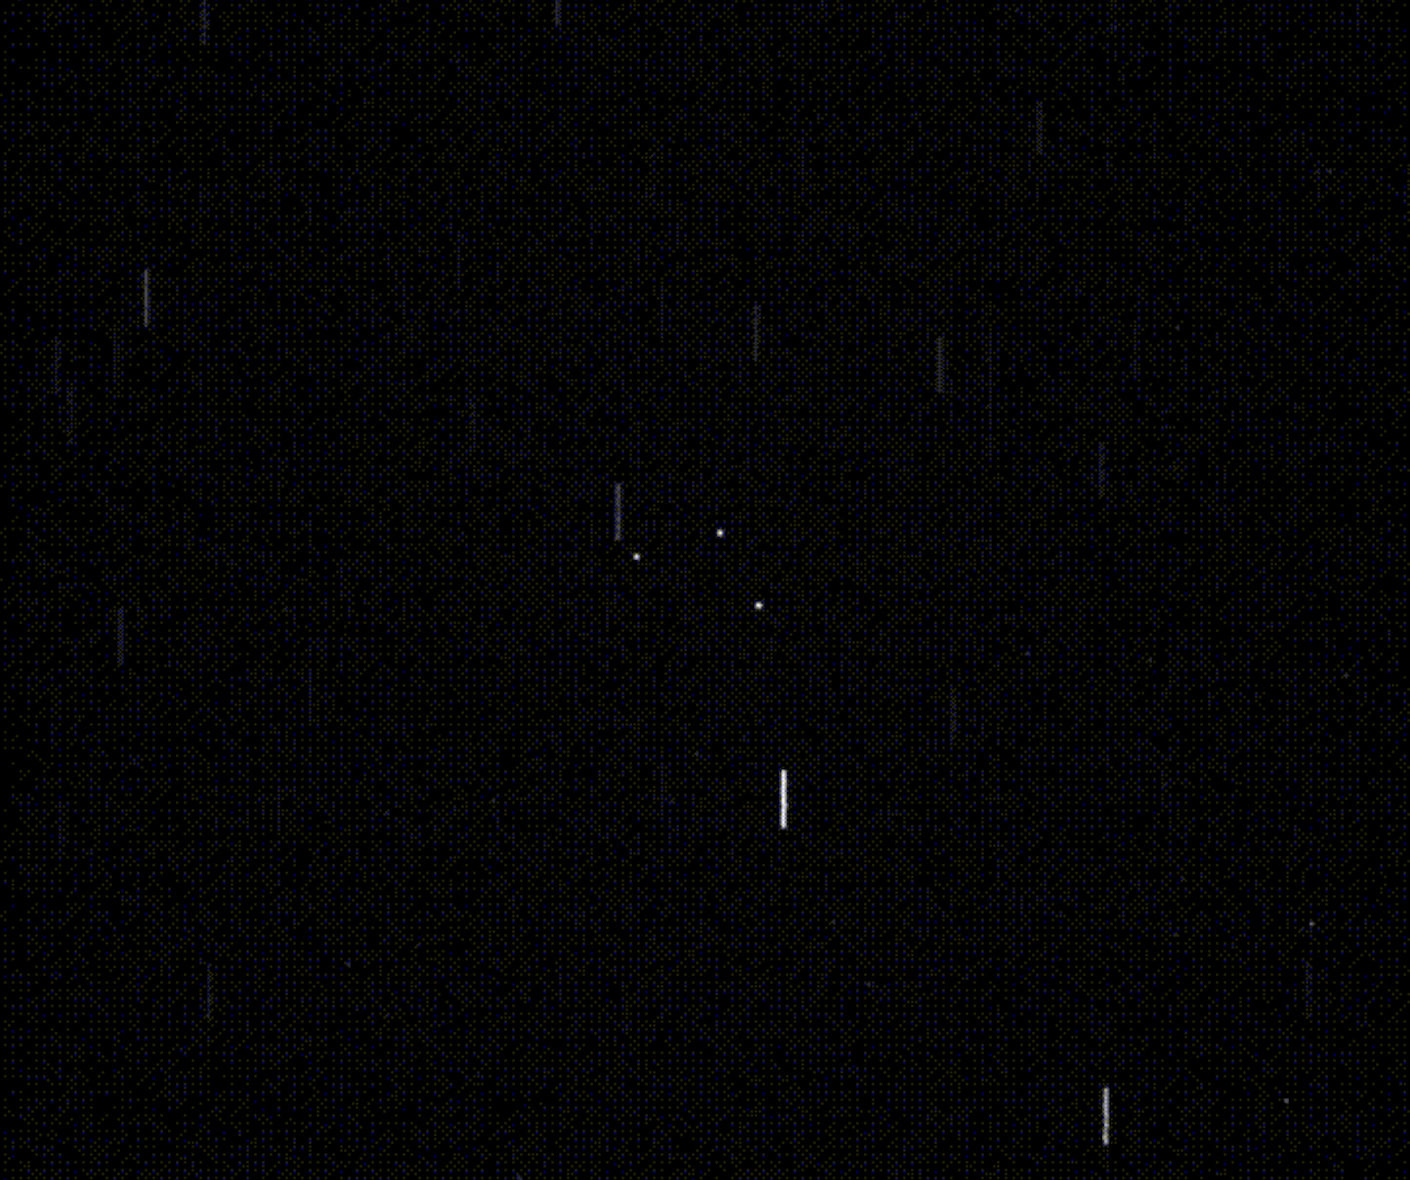
\includegraphics[width=\figmed]{static_images/static_pogs_raw_image.png}
  \caption{Raw image of three GEO objects with stars streaking through the background. Taken by the Purdue Optical Ground station at \pogslla by Nathan Houtz}
  \label{fig:pogs_observation_example}
\end{figure}

In Figure \ref{fig:pogs_observation_example}, most stars are too faint to appear as points of light on the image plane. Instead, they merge into the background. The signal due to these faint stars is known as integrated starlight.
Krag \cite{krag2003} modeled this signal by building a $1^\circ \times 1^\circ$ grid of surface
brightness values for the full right ascension (RA) and declination (Dec) sphere. Krag used the
Guide Star catalog, which contains 15 million stars down to magnitude 16. Exponential extrapolation
was used to predict star counts in each bin for higher magnitudes \cite{krag2003}. Twenty years later, larger star catalogs exist that are nearly complete to much dimmer magnitudes. The integrated
starlight catalog used in this work was built from the GAIA catalog with approximately 1.5 billion
stars down to magnitude 21-22 \cite{gaia_dr3}. The same $1^\circ \times 1^\circ$ grid was computed
using the \texttt{astroquery.gaia} Python package \cite{astroquery_gaia}. Figure
\ref{fig:gaiapatched} shows the computed brightness map, in units of $S_{10}$. 

\begin{figure}[ht]
  \centering
  \includegraphics[width=\figbig]{sphx_glr_gaia_patched_catalog_001_2_00x.png}
  \caption{Integrated starlight brightness map}
  \label{fig:gaiapatched}
\end{figure}

With this map of exoatmospheric mean brightness of the night sky due to integrated
starlight, the corresponding signal mean in the telescope CCD is computed, adopting Krag's formulation \cite{krag2003}.

\begin{equation} \label{eq:bint}
 \textrm{BINT} = \frac{\pi D^2}{4}
  \int_{10^{-8}}^{10^{-6}}{ \textrm{STRINT}(\lambda) \cdot \textrm{QE}(\lambda) \cdot \textrm{ATM}(\lambda)
  \cdot \left( \frac{\lambda}{h c} \right) \: d\lambda}  
\end{equation}

In Eq \ref{eq:bint}, $D$ is the telescope aperture diameter in meters, $h$ is Plank's constant in
$\left[ \frac{m^2 kg}{s} \right]$, and $c$
is the speed of light in vacuum in $\left[ \frac{m}{s} \right]$. The resulting quantity
$\textrm{BINT}$ has units of $\left[ \frac{1}{s} \right]$, representing the mean total photons passing
through the telescope aperture due to integrated starlight. 

\begin{equation} \label{eq:starlightmean}
  \bar{S}_{star} = 10^{-4} \cdot BINT \cdot \left( \frac{s_{pix}}{3600} \right)^2 \cdot \Delta t \cdot
  b_{cat}
\end{equation}

In Eq \ref{eq:starlightmean}, $b_{cat}$ is the patched catalog brightness in $\left[ S_{10}
\right]$, $s_{pix}$ is the telescope pixel scale in $\left[ \frac{arcsecond}{pix} \right]$, and $\Delta t$ is the integration time in seconds. Note the addition of the $10^{-4}$ factor to reconcile catalog surface brightness in terms of 10th magnitude stars, and the 0th magnitude source in $\textrm{BINT}$. This yields $\bar{S}_{star}$ with units $\left[ \frac{e^-}{pix^2} \right]$; photoelectron counts (ADU) per pixel. Figure \ref{fig:starlight_hemi} shows the background signal mean due to integrated starlight.

\begin{figure}[ht]
  \centering
  \includegraphics[width=\figmed]{sphx_glr_background_signals_002.png}
  \caption{Integrated starlight signal on the local observer hemisphere. The observer is in New Mexico, USA at
  \pogslla}
  \label{fig:starlight_hemi}
\end{figure}

\subsection{Scattered Moonlight}

Moonlight scattering through the atmosphere significant increases background brightness \cite{krag2003}. This scattering effect can be decomposed into Rayleigh (isotropically distributed) and Mie (exponentially distributed) scattering modes. The Rayleigh scattered component is computed with Table 4 published by Daniels parameterized by the angle from the observation to zenith $z_{obs}$, the angle from the Moon to zenith $z_{moon}$, and the angle between the observation and the Moon on the horizon $\Delta Az$ \cite{daniels1977}. Interpolating this table yields the intensity of the Rayleigh scattering $F_{rs}$ in $10^{-10}$ $W/(cm^2 \cdot \mu m \cdot sr)$ \cite{krag2003}. The Mie scattered component is formulated with Eq \ref{eq:mie_scattering_moon}.

\begin{equation} \label{eq:mie_scattering_moon}
  F_{ms}(\lambda) = a_1 \left[ e^{-\left(\frac{\Psi}{\Psi_1}\right)} + a_2 e^{-\left(\frac{\pi - \Psi}{\Psi_2}\right)} \right] F_{rs}(\lambda)
\end{equation}

Daniels recommends $a_1 \in [50, 100]$, $a_2 \in [0.01, 0.02]$, $\Psi_1 \in [10^\circ, 20^\circ]$, and $\Psi_2 \approx 50$ \cite{daniels1977}. Prior to any station-specific fitting, the middle of these intervals are chosen, yielding $a_1 = 75$, $a_2 = 0.015$, $\Psi_1 = 15^\circ$, and $\Psi_2 = 50^\circ$. $a_1$ and $a_2$ are dimensionless, such that $F_{ms}$ also has units of $10^{-10}$ $W/(cm^2 \cdot \mu m \cdot sr)$. The total intensity of the scattered moonlight $F_{mt}$ via Eq \ref{eq:total_scattered_moonlight} following Krag's formulation \cite{krag2003}.

\begin{equation} \label{eq:total_scattered_moonlight}
  F_{mt} = f(\theta) \left[ F_{rs}(\lambda) + F_{ms}(\lambda) \right]
\end{equation}

in Eq \ref{eq:total_scattered_moonlight}, $f(\theta)$ is the lunar phase function which describes the fraction of the full Moon brightness is reflected at an observer viewing the Moon an angle $\theta$ from the Sun vector. This function is linearly interpolated within Table 3 in \cite{daniels1977}. Finally, Krag introduces a correction factor $f_{corr}$ to account for the difference between the Sun's irradiance spectrum and the spectrum of scattered moonlight, defined in Eq \ref{eq:krag_f_corr}.

\begin{equation} \label{eq:krag_f_corr}
  f_{corr} = \frac{I_0}{SUN(550 \: \left[\textrm{nm}\right])}
\end{equation}

With all these pieces, the mean scattered moonlight signal in ADU per pixel is computed in Eq \ref{eq:moonlight_adu}.

\begin{equation} \label{eq:moonlight_adu}
  \bar{S}_{moon} = F_{mt}(550 \: \left[\textrm{nm}\right]) \cdot SINT \cdot \left( \frac{s_{pix}}{3600} \right)^2 \cdot \Delta t \cdot f_{corr}
\end{equation}

\begin{figure}[ht]
  \centering
  \includegraphics[width=\figmed]{sphx_glr_background_signals_001.png}
  \caption{Mean scattered moonlight signal on the local observer hemisphere. The observer is in New Mexico, USA at
  \pogslla}
  \label{fig:moonlight_hemi}
\end{figure}

\subsection{Zodiacal Light}

Zodiacal light is an effect created by sunlight reflecting off of dust in the ecliptic plane \cite{krag2003}. Zodiacal light is strongest around the Sun --- an area that is not of interest --- but also reaches a peak directly away from the Sun due to the opposition effect. This peak is known as the Gegenschein, meaning "opposing light". The zodiacal light brightness is linearly interpolated within Table 1 of \cite{roach1972}. This reports the surface brightness of the zodiacal light in $S_{10}$, which is used without conversion to find the mean CCD signal in ADU per pixel via Eq \ref{eq:zodiacal_adu}.

\begin{equation} \label{eq:zodiacal_adu}
  \bar{S}_{zod} = BINT \cdot \left( \frac{s_{pix}}{3600} \right)^2 \cdot \Delta t \cdot ZOD \cdot 10^{-4}
\end{equation}

As in the integrated starlight signal, the $10^{-4}$ factor reconciles the $S_{10}$ surface brightness with the 0th magnitude source in $\textrm{BINT}$. 

\begin{figure}[ht]
  \centering
  \includegraphics[width=\figmed]{sphx_glr_background_signals_004.png}
  \caption{Mean zodiacal light signal on the local observer hemisphere. The observer is in New Mexico, USA at
  \pogslla}
  \label{fig:zod_hemi}
\end{figure}

\subsection{Sampling Background}

Notice that each background signal is only defined in terms of its mean. On a pixel-by-pixel basis, the signal for an exposure is sampled from a Poisson distribution for each background term. This distribution can be interpreted as modeling the number of independent events that occur during a time period. In our case, this translates to individual photons being incident on our sensor. A Poisson distribution is defined on the positive integers by a single parameter $\lambda$ which is both the mean and variance of the distribution. The probability density function (PDF) for the Poisson distribution takes the form of Eq \ref{eq:poisson_pdf} \cite{frueh2019notes}.

\begin{equation} \label{eq:poisson_pdf}
  P_\lambda(x=k) = \frac{\lambda^k e^{-\lambda}}{k!}
\end{equation}

This distribution has a useful property that $P_{\lambda_1 + \lambda_2}(x=k) = P_{\lambda_1}(x=k) + P_{\lambda_2}(x=k)$ so long as the distributions described by $\lambda_1$ and $\lambda_2$ are independent. Since our background sources are assumed to be independent as sources like moonlight and zodiacal light are clearly distinct; if the Moon vanished, interplanetary dust across the solar system would reflect light identically. As a result, the total background signal is equivalent to a single Poisson variable.

\begin{equation} \label{eq:background_poisson}
  \lambda_{background} = \bar{S}_{airglow} + \bar{S}_{pollution} + \bar{S}_{twilight} + \bar{S}_{star} + \bar{S}_{moon} + \bar{S}_{zod}
\end{equation}

Drawing samples from the Poisson distribution defined by $\lambda_{background}$ computes the background of the CCD image. 

\subsection{Background Source Importance}

Some background signals are more impactful than others. Table \ref{tb:signal_importance} details the approximate magnitudes in photoelectrons per pixel one can expect from a telescope similar to the Purdue Optical Ground Station.

\begin{table}[] \label{tb:signal_importance}
  \begin{tabular}{|l|l|}
  \hline
  \textbf{Signal source} & \textbf{Magnitude} $\mathbf{\left[ e^- / \textbf{pix}\right]}$ \\ \hline
  Airglow                & $10^3 - 10^4$                              \\ \hline
  Scattered moonlight    & $0 - 10^5$                                 \\ \hline
  Integrated starlight   & $10^1 - 10^2$                              \\ \hline
  Light pollution        & $10^2 - 10^3$                              \\ \hline
  Zodiacal light         & $10^2 - 10^4$                              \\ \hline
  Twilight               & $10^1 - 10^7$                              \\ \hline
  \end{tabular}
  \caption{Background signal importance}
\end{table}

\section{Sensor Effects}

\subsection{Dark Noise}

TODO

\subsection{Readout Noise}

TODO

\section{Signal to Noise Ratio (SNR)}

TODO

\section{Sampling Noisy Light Curves}

TODO

%%% METHOD
\ProvidesFile{ch-light-curve-simulation.tex}[Light Curve Simulation]
\graphicspath{{/Users/liamrobinson/Documents/PyLightCurves/docs/build/html/_images}}

\section{Light Curve Simulation}

\subsection{Orbital Dynamics}

TODO

\subsection{Discrete Shape Representations}

A computer can represent 3D objects implicitly or explicitly. An implicit representation might be the solution to an algebraic equation, i.e., $x^2 + y^2 + z^2 = 1$ defines a sphere of radius $1$ centered at the origin. Often, a shape may be defined by a set of signed distance functions (SDFs). An SDF takes in a point in \rthree and outputs the distance from the object, returning negative distance if the queried point is inside the shape. The object can then be rendered via ray marching. A ray is cast from the camera out into the scene for each pixel of the screen, each performing distance queries along its length until it intersects the object or diverges. 

By contrast, an explicit shape representation creates complex 3D geometry from simple 2D building blocks. In the most common case, object faces are defined by triangles. This means that at the scale of the individual faces, the shape is always composed of flat surfaces that meet at sharp angles. While this can add complexity to many fields of shape analysis and geometry processing, triangulated surfaces are perfect for our application. Human-made space objects like most satellites are composed of flat faces, with the exception of parabolic antennas and cylindrical rocket bodies.

\subsubsection{The Object File Format}

One common text file format for 3D model files is \texttt{.obj}, developed by Wavefront Technologies in the early 1990s \cite{obj_format}. Each OBJ file consists of a list of vertex positions and face definitions, with optional vertex normals and tangents. An \texttt{.obj} listing for a cube is included for reference in Appendix \ref{sec:obj_listing}. Given the vertex positions and adjacency information stored in the model file, useful properties of the object can be computed for use later in both light curve simulation and shape inversion. 

\subsubsection{Properties of Triangulated Meshes}

For each triangular face $F_i$ of the model defined by vertices $F_i = \left\{v_1, v_2, v_3\right\}$, the outward-pointing face normal is computed with

\begin{equation} \label{eq:face_normal}
    \hat{n} = \frac{\left( v_2 - v_1 \right) \times \left( v_3 - v_1 \right)}{\| \left( v_2 - v_1 \right) \times \left( v_3 - v_1 \right) \|_2}.
\end{equation}

The face area is computed with

\begin{equation} \label{eq:face_areas}
    a = \frac{\| \left( v_2 - v_1 \right) \times \left( v_3 - v_1 \right)\|_2}{2}.
\end{equation}

The support of the $i$th face --- the perpendicular distance from the origin to the plane defining the face --- is computed with the position of any vertex on that face, i.e., the first vertex $v_{i,1}$, and the face normal vector $\hat{n}_i$

\begin{equation} \label{eq:face_support}
    h_i = v_{i,1} \cdot \hat{n}_i.
\end{equation}

The volume of the object is computed with

\begin{equation} \label{eq:object_volume}
    V = \frac{1}{3} \sum_{i=0}^{ \lvert F \rvert}\vec{h}_i \cdot \vec{a}_i.
\end{equation}

In Eq \ref{eq:object_volume}, $\lvert F \rvert$ is the number of faces defining the object. $\vec{h}$ and $\vec{a}$ are column vectors collecting all face supports and areas. The Extended Gaussian Image, a quantity defined in \ref{sec:egi_definition}, is computed row-wise for the $i$th face with

\begin{equation} \label{eq:egi_definition}
    \vec{E}_i = \vec{a}_i \vec{n}_i.
\end{equation}

\subsection{Selected Satellite Models}

Most of the analysis in this work used one of the 3D model files shown in Figure \ref{fig:satellite_lineup}. Figure \ref{fig:satellite_lineup} highlights the size of the GEO communications satellites (TELSTAR, HYLAS, Hispasat, and ASTRA). In contrast, the LEO satellites (Starlink and Landsat) are dwarfed at the left end of the lineup.

\begin{figure}[ht]
    \centering
    \includegraphics[width=\figbig]{sphx_glr_satellite_lineup_001.png}
    \caption{Selected space objects with soccer field for size reference. In order, the objects are TESS, Starlink V1, TDRS, Landsat 8, Hispasat 30W-6, Saturn V SII, TELSTAR 19V, HYLAS 4, and simplified ASTRA.
    }
    \label{fig:satellite_lineup}
\end{figure}

\subsection{The Bidirectional Reflectance Distribution Function}

Although light curves come from unresolved measurements, the interactions that produce them are directly driven by the shape and material properties of the object being observed. In order to simulate accurate light curves, all relevant optical interactions must be modeled. In broad terms, this boils down to determining how the object is illuminated, how it casts shadows on itself, and how it is observed. 

At the microscopic scale, the surface of an object is composed of facets ---  small areas sharing a normal vector. The macroscopic optical properties of the material is driven by the distribution of sizes and normal directions of these microfacets. If the facet normals are distributed in biased orientations, the macroscopic surface may show anisotropy, leading to the appearance of brushed metal. If the facets normals are at large angles to each other, the surface may appear dull as the direction of the outgoing light may be largely independent from the incoming direction. Subsurface effects ---  where incoming light rays scatter \textit{inside} the surface can also change the macroscopic properties of the material. 

This discussion raises an important question; how should the macroscopic outcomes of the microscopic interactions of incident light on a surface be modeled? The bidirectional reflectance distribution function (BRDF) is a tool from computer graphics that addresses this problem. The BRDF is a function on the hemisphere which expresses the fraction of light per solid angle (radiance $\mathcal{R}$) leaving the surface in a given direction, divided by the incident power per unit area (irradiance $\mathcal{I}$). The general formulation for a BRDF $f_r$ is given by Eq \ref{eq:brdf_def} \cite{duvenhage2013}.

\begin{equation}
    f_r(\vctr{x}, L \rightarrow O) = \frac{d\mathcal{R}\left(\vctr{x} \rightarrow O\right)}{d\mathcal{I}\left(L \rightarrow \vctr{x}\right)}
    \label{eq:brdf_def}
\end{equation}

In Eq \ref{eq:brdf_def}, $\vctr{x} \in \mathbb{R}^3$ is the point on the object's surface where the BRDF is evaluated. $L \in \mathbb{S}^2$ is the incoming illumination unit vector and $O \in \mathbb{S}^2$ is the outgoing unit vector. Note that this work treats $f_r(\vctr{x}, L \rightarrow O)$ and $f_r(L \rightarrow O)$ as equivalent in later descriptions, leaving the evaluation point $\vctr{x}$ implied. This definition is useful for building intuition about the form of the BRDF, but to represent a physically plausible reflection process, a candidate function must satisfy three additional constraints. A physically plausible BRDF must conserve energy --- more energy cannot be reflected from the surface than was incident on it. It must also be reciprocal --- switching the observer and illumination directions should not change the BRDF value as the surface interaction. This reciprocity is sometimes known as the \textit{Helmholtz Reciprocity Rule} in literature \cite{montes2012}. Finally, plausible BRDFs are positive --- they take on nonnegative values for all valid inputs \cite{montes2012}. A surface cannot reflect negative light, so this should feel natural. Explicitly, energy conservation is expressed by Eq \ref{eq:brdf_energy_cons} \cite{montes2012}.

\begin{equation} \label{eq:brdf_energy_cons}
  \forall L \in \mathbb{S}^2 : \:\: \int_{O \in \mathbb{S}^2} f_r(L \rightarrow O) \: d\mathbb{S}^2 \leq 1
\end{equation}

Eq \ref{eq:brdf_energy_cons} states that for all possible illumination directions $L$, integrating all possible outgoing observer directions $O$ on the unit sphere cannot return greater than one from the energy conservation integral. Reciprocity can also be formalized via \ref{eq:brdf_reciprocity}.

\begin{equation} \label{eq:brdf_reciprocity}
  \forall L, O \in \mathbb{S}^2 : \:\: f_r(L \rightarrow O) = f_r(O \rightarrow L)
\end{equation}

\subsection{BRDF Formulations}

Now that the requirements for a plausible physical BRDF have been established, a collection of commonly-used BRDFs can be presented. The following BRDFs are all energy conserving, reciprocal, and nonnegative. This does not mean that they are always sufficient for modeling real-world materials, they merely represent ways hypothetical surfaces could reflect light without breaking any fundamental physics.

\subsubsection{Lambertian}

The simplest BRDF is one that reflects equally in all directions. This BRDF is termed Lambertian or diffuse.

\begin{equation} \label{eq:brdf_lambertian}
  f_r(L \rightarrow O) = \frac{C_d}{\pi}
\end{equation}

In Eq \ref{eq:brdf_lambertian}, $0 \leq C_d \leq 1$ is the surface's coefficient of diffuse reflection. For example, $C_d = 0.4$ means that the surface reflects $40\%$ of incident radiation and absorbs the other $60\%$. 

\subsubsection{Phong}

While the diffuse BRDF reflects energy isotropically, many real-world reflections are highly biased. At the extreme end, a perfect mirror reflection is effectively a Dirac delta function in the reflected illumination direction. Many real-world materials are well-modeled as a linear combination of diffuse and specular effects. A simple specular BRDF model is that developed by Phong in 1975 \cite{phong1975}. The Phong model splits the BRDF into a Lambertian term governed by $C_d$ and a specular term governed the coefficient of specular reflection $ 0 \leq C_s \leq 1$ and the specular exponent $n \geq 0$ \cite{duvenhage2013}. 

\begin{equation} \label{eq:brdf_phong}
  f_r(L \rightarrow O) = \frac{C_d}{\pi} + \frac{C_s \frac{n+2}{2\pi} (O \cdot R)^n}{N \cdot L}
\end{equation}

In Eq \ref{eq:brdf_phong}, $R$ is the reflected illumination vector, computed via $R = 2 (N \cdot L) N - L$. As $n$ increases, the specular glint becomes sharper and more intense, eventually approaching a perfectly mirror reflection. Because of the introduction of a new coefficient of reflection, a new constraint is needed to maintain energy conservation. Because $C_d$ and $C_s$ each represent the \textit{fraction} of light reflected in each mode, it should be clear that $C_d + C_s \leq 1$. This can also be reformulated with an explicit coefficient of absorption $C_a$ which captures the fraction of incident radiation absorbed by the surface, yielding $C_d + C_s + C_a = 1$. 

\subsubsection{Blinn-Phong}

The Blinn-Phong BRDF is similar to to the Phong BRDF, but parameterizes the specular lobe in terms of the halfway vector $H$ \cite{duvenhage2013}. This vector is halfway between the illumination and observer directions such that $H = L + O$ which needs to be normalized before use. As the halfway vector approaches the surface normal vector, the observer must be approaching the reflected illumination vector, leading to a more intense specular highlight. 

\begin{equation} \label{eq:brdf_blinn_phong}
  f_r(L \rightarrow O) = \frac{C_d}{\pi} + \frac{C_s \frac{n+2}{2\pi} (N \cdot H)^n}{4 (N \cdot L)(N \cdot O)}
\end{equation}

\subsubsection{Glossy}

The so-called glossy BRDF simulates reflections from plastic materials using an Gaussian distribution around the specular scattering lobe \cite{duvenhage2013}. In Eq \ref{ref:eq_brdf_glossy}, the parameter $\sigma$ controls the width of the specular Gaussian.

\begin{equation} \label{eq:brdf_glossy}
  f_r(L \rightarrow O) = \frac{C_d}{\pi} + \frac{C_s}{2\pi \sigma^2 \left(N \cdot L\right)}  e^{\frac{-\left( R \cdot O \right)^2}{2\sigma^2}}
\end{equation}

\subsubsection{Cook-Torrance}

The Cook-Torrance explicitly accounts for the orientation of the microfacets making up the surface \cite{cook1982}. This model is built from a facet slope distribution term $D$, a Fresnel term $F$, and a geometric attenuation factor $G$. The slope distribution term describes the probability density of a given facet being oriented with a normal vector aligned with the halfway vector $H$ \cite{cook1982}. A common formulation of this term is due to Beckmann:

\begin{equation} \label{eq:d_beckmann}
  D = \frac{1}{\pi \alpha^2 \left( N \cdot H \right)^4} \exp\left( \frac{1 - \left(N \cdot H\right)^2}{\alpha^2 \left(N \cdot H\right)^2} \right).
\end{equation}

In Eq \ref{eq:d_beckmann}, $\alpha \in [0, 1]$ is the roughness of the surface \cite{cook1982}. The Fresnel term accounts for the variation in specular reflection due to the angle of incidence. In reality, this term is a function of wavelength, but is often approximated as \cite{cook1982}:

\begin{equation} \label{eq:fresnel_approx}
  F = C_s + \left( 1 - C_s \right) \left( 1 - \left( H \cdot L \right) \right) ^ 5.
\end{equation}

The geometric attenuation term expresses how microfacets shadow eachother, and can be approximated with \cite{cook1982}:

\begin{equation} \label{eq:cook_torrance_g}
  G = \min \left\{ 1, \frac{2\left(N \cdot H\right) \left(N \cdot O\right)}{O \cdot H}, \frac{2\left(N \cdot H\right) \left(N \cdot L\right)}{O \cdot H} \right\}.
\end{equation}

The overall reflectance for the Cook-Torrance BRDF is given by:

\begin{equation} \label{eq:brdf_cook_torrance}
  f_r(L \rightarrow O) = \frac{C_d}{\pi} + \frac{D \cdot G \cdot F}{4 \left(N \cdot L\right) \left( N \cdot O \right)}
\end{equation}

\subsubsection{Oren-Nayar}

The Oren-Nayar BRDF is an improved model of diffuse reflectance for many real-world materials like ceramics and the surface of the Moon. These materials diverge from the Lambertian model near the horizon, reflecting much more light than would be predicted by simple cosine loss \cite{oren1994}. This BRDF relies on the surface roughness $\alpha$ to compute a set of constants \cite{oren1994}:

\begin{align*} \numberthis
  A &= 1 - 0.5 * \frac{\alpha^2}{\alpha^2 + 0.33} \\
  B &= 0.45 * \frac{\alpha^2}{\alpha^2 + 0.09} \\
  C &= \frac{\mathrm{proj}_{N}\left(L\right)}{\|\mathrm{proj}_{N}\left(L\right)\|} \cdot  \frac{\mathrm{proj}_{N}\left(O\right)}{\|\mathrm{proj}_{N}\left(O\right)\|}. \\
  \beta &= \max \left\{ \arccos\left( L \cdot N \right), \: \arccos\left( O \cdot N \right) \right\} \\
  \gamma &= \min \left\{ \arccos\left( L \cdot N \right), \: \arccos\left( O \cdot N \right) \right\} \\
\end{align*}

With these values computed, the reflectance of the Oren-Nayar BRDF is given by \cite{oren1994}:

\begin{equation}
  f_r(L \rightarrow O) = \frac{C_d}{\pi} \left(A + (B \max\left\{C, 0\right\} \sin\beta \tan\gamma) \right)
\end{equation}

\subsubsection{Ashikhmin-Shirley}

The Ashikhmin-Shirley BRDF is unique among those presented in this section as it allows for anisotropic reflection which can be non-negligible for metals \cite{ashikhmin2000}. This model is parameterized by the diffuse reflection coefficient, as well as two specular exponents $n_u$ and $n_v$. When $n_u = n_v$, the model behaves much like the Phong BRDF. The full BRDF is expressed \cite{ashikhmin2000}:

\begin{align*} \numberthis \label{eq:brdf_ashikhmin_shirley}
  \rho_d &= \frac{28 C_d}{23 \pi} (1 - C_s) \left(1 - \left(1 - \frac{N \cdot L}{2}\right)^5\right) \left(1 - \left(1 - \frac{N \cdot O}{2}\right)^5\right) \\
  \rho_s &= \frac{\sqrt{(n_u+1)(n_v+1)}}{8 \pi} \frac{\left( N \cdot H \right)
  ^\frac{n_u \left(H \cdot U \right)^2 + n_v \left( H \cdot V \right)^2}{1 - \left(H \cdot N\right)^2}}
  {\left(H \cdot L\right) \max\left\{ N \cdot O, N \cdot L \right\}} F \\
  f_r(L \rightarrow O) &= \rho_d + \rho_s. \\
\end{align*}

In Eq \ref{eq:brdf_ashikhmin_shirley}, $F$ is the same Fresnel factor in Eq \ref{eq:fresnel_approx} while $U$ and $V$ are predefined surface basis vectors perpendicular to the surface normal.

\subsection{BRDF Summary}

\begin{figure}[ht]
  \centering
  \includegraphics[width=\figbig]{sphx_glr_brdf_renders_002_2_00x.png}
  \caption{Implemented BRDFs rendered with arbitrary parameters, demonstrating the qualitative differences between lighting models}
  \label{fig:brdf_renders}
\end{figure}

\subsection{Simulating Light Curves for Convex Objects}

Light curve simulation for convex geometry can be solved semi-analytically as each face's contribution 
to the measured irradiance can be computed individually \cite{kaasalainen2001}. 
Determining whether a face is illuminated requires two horizon checks to determine visibility 
from the Sun and to the observer. For a face $i$ at timestep $j$ these horizon checks are 
expressed by the shadowing condition $\mu_{ij}$. 

\begin{equation} \label{eq:cvx_shadow_cond}
  \mu_{ij} = \begin{cases}
    1 \text{ if } \left( O_j \cdot \hat{n}_i \right) > 0 \text{ and } \left( L_j \cdot \hat{n}_i \right) > 0 
	  \text{ and } \delta_{ij,\text{ss}} = 0 \text{ and } \delta_{ij,\text{os}} = 0\\
    0 \text{ otherwise } \\
  \end{cases}
\end{equation}

The unit vectors $O$ and $L$ point from the center of mass of the object to the observer and Sun, respectively. 
We choose the outward-pointing face normal unit vector $\hat{n}$ by convention for all mesh operations. 
The self-shadowing and observer-shadowing conditions, $\delta_{ij,\text{ss}}$ and $\delta_{ij,\text{os}}$, 
are always zero for convex polyhedra but are crucial for accurately simulating nonconvex geometry. 
For objects with concavities, self-shadowing refers to shadows cast by an object onto itself and observer-shadowing 
refers to otherwise visible faces blocked by other portions of the geometry.

The irradiance $I$ received by the observer at timestep $j$ is the sum of the received irradiance from all faces, 
composed of specular and diffuse contributions. Each contribution is expressed as the product of the
normalized irradiance $\hat{I}$. This can be scaled to adjust for the distance from the observer to
the object to yield the noiseless received irradiance.

TODO: add L = Ga stuff

\subsection{Simulating Light Curves for nonconvex Objects}

Many existing light curve simulation methods for nonconvex objects rely on ray tracing schemes like Möller and Trumbore's ray-triangle intersection algorithm \cite{moller2005,fan2020thesis}. This computation has complexity $\mathcal{O}(n^2)$ if implemented naïvely, but can be improved to $\mathcal{O}(n \ln n)$ with better spatial data structures. For human-made space objects, there may be significant self-shadowing at large phase angles. As a result, it cannot be assumed that the self-shadowing conditions $\delta_{ij,\text{ss}}$ and $\delta_{ij,\text{os}}$ are zero \cite{frueh2014,fan2020thesis}. Naïve ray traced shadows generally require $\mathcal{O}(n^2)$ ray-triangle intersections per timestep for $n$ faces. For this reason, ray traced shadows quickly become infeasible for complex objects without GPU parallelization. The limitations of ray-triangle intersections for light curve simulation is discussed at length by Frueh et al. \cite{frueh2014}.

\graphicspath{{/Users/liamrobinson/Documents/msthesis/static_images/aas_2022_figs}}
\begin{figure}[!htb]
  \centering
  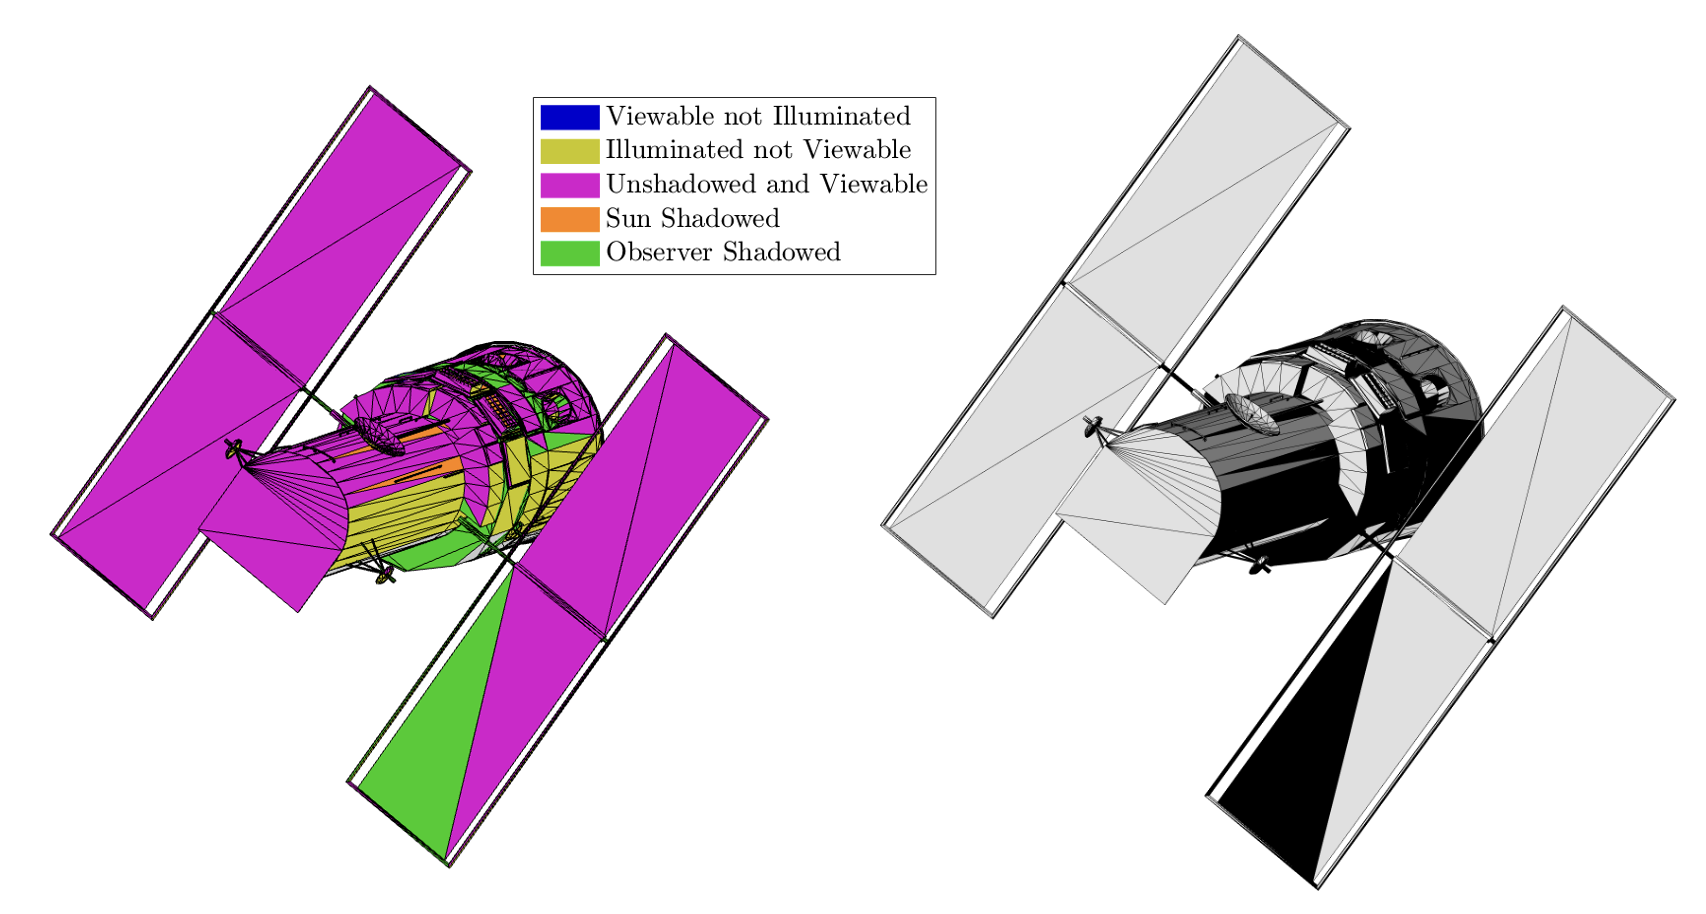
\includegraphics[width=350px]{hst_shadow_mapping/composite_hst_raytraced.png}
  \caption{Hubble Space Telescope ray traced shadow categorization and shading. Models from \cite{nasa_models}}
  \label{hst_shadows_ray}
\end{figure}

\subsection{The Importance of Self-Shadowing}

To motivate the need for accurate shadows when dealing with human-made space objects, consider the error introduced by neglecting shadows for different types of space objects. Kaasalainen and Torppa's work on asteroids reasonably assumed that shadowing was a negligible contribution to the measured light curve. Human-made objects do not afford the same luxury. Figure \ref{fig:hst_bennu_shadows} displays light curves for the asteroid Bennu and the Hubble Space Telescope with and without accurate shadows under a single-axis spin profile with inertially fixed Sun and observer vectors. Without accurate shadowing, the light curve's intensity and its time derivative can be significantly error-prone.

\begin{figure}[!htb]
  \centering
  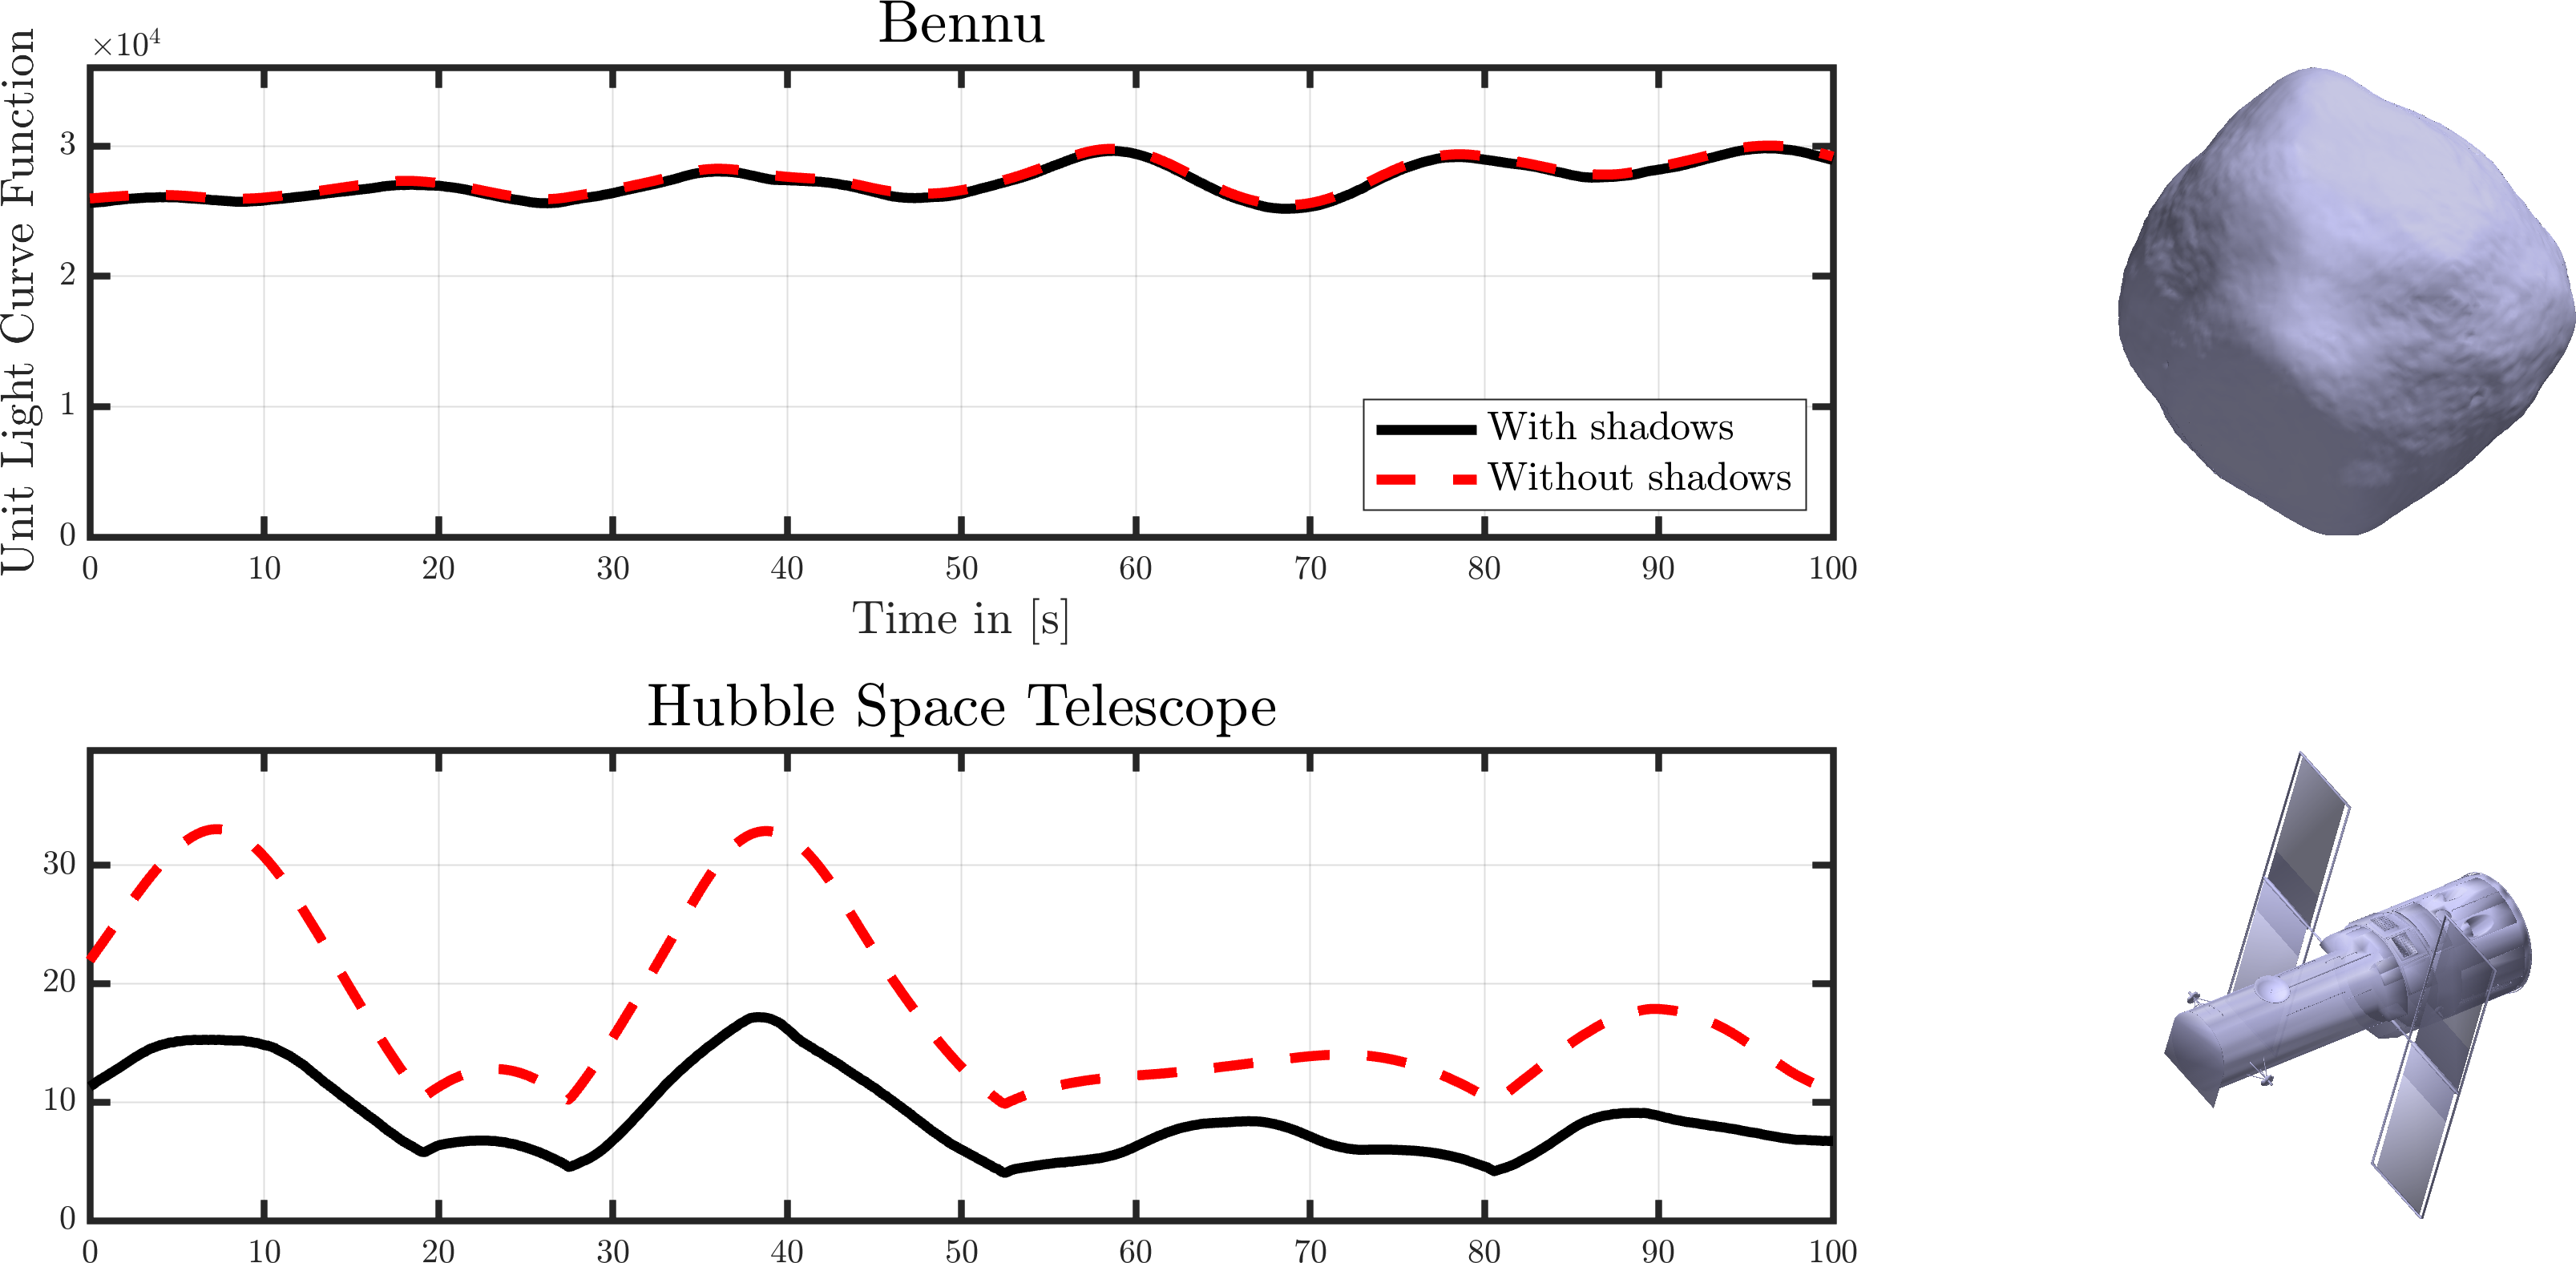
\includegraphics[width=350px]{convex_vs_nconv_lcs.png}
  \caption{Brightness errors introduced by neglecting shadows for Bennu and HST. Models from \cite{nasa_models}}
  \label{fig:hst_bennu_shadows}
\end{figure}

\subsection{Shadow Mapping}

Shadow mapping is used in the simulations presented in this work for faster and more accurate self-shadowing. Shadow mapping is a well understood technique in computer graphics \cite{kolivand2013}. Although modern ray traced shadowing may be more computationally efficient, shadow mapping was selected for its ease of implementation \cite{kolivand2013}. Shadow mapping shades individual pixel fragments instead of entire faces, offering increasing shadow quality over facewise ray tracing as the number of mesh faces falls.

Given an observer and Sun vector in the body frame of the object, shadow mapping proceeds in a four step process. In step one, a camera is positioned along the Sun vector and a perpendicular depth texture is computed. In the second step, depth values in Sun camera space are transformed to observer camera space, where a second depth texture is computed. This second texture is used to find the closest fragment along each ray to the Sun \cite{brabec2002}. Self-shadowed fragments are classified as those further from the Sun than the closest fragment along the same ray, indicated in red in Figure \ref{fig:hst_shadows_map}. Fragments that do not pass the convex shadowing condition are horizon shadowed, indicated in blue in Figure \ref{fig:hst_shadows_map}, determining the Sun and observer shadowing conditions at once. All remaining fragments are shaded with using the same Lambertian reflection model in \ref{eq:lc_func_diffuse} TODO: this equation is broken. Computing the light curve function for the final rendered image requires summing all pixel values and dimensionalizing the result by the area of the observer camera's field of view. The light curve simulation environment used in this work was implemented in C and OpenGL \cite{raylib}.

In order to compute the final shaded and shadowed image, a depth map must be computed from the perspective of two orthographic cameras in the Sun and observer directions. These depth masks require a set of transformations from the model body frame to screen space. With this background laid out, the process for computing a perpendicular depth map $d(x,y)$ from the perspective of an arbitrary orthographic camera is detailed in Algorithm \ref{alg:depth_map}.

\begin{algorithm}
  \caption{Depth map for shadow mapping} \label{alg:depth_map}
  \begin{algorithmic}
    \State $(x, y) \in \mathbb{Z}$ \Comment{Pixel coordinates on the image plane}
    \State $R_{pix} \in \mathbb{R}^3$ \Comment{Pixel world coordinates; provided by OpenGL}
    \State $d(x, y) \gets \left( R_{cam} - R_{pix} \right) \cdot R_{cam}$ \Comment{Pixel depth in the camera view direction}
  \end{algorithmic}
\end{algorithm}

The pixel-wise shading process is summarized in Algorithm \ref{alg:pix_shading}.

\begin{algorithm}
  \caption{Pixel-wise shading algorithm with shadow mapping}\label{alg:pix_shading}
  \begin{algorithmic}
    \State $L \in \mathbb{S}^2$ \Comment{Unit vector from object origin towards Sun}
    \State $O \in \mathbb{S}^2$ \Comment{Unit vector from object origin towards observer}
    \State $N \in \mathbb{S}^2$ \Comment{Outward-pointing surface normal vector at pixel coordinates}
    \State $(C_d, C_s, n) \in \mathbb{S}^2$ \Comment{Reflection coefficients and exponent for the BRDF}
    \Require $C_d + C_s \leq 1$ \Comment{Enforce energy conservation}
    \State $MVP_{Sun} \in \mathbb{R}^{4 \times 4}$ \Comment{MVP matrix for the Sun camera}
    \State $(x, y) \in \mathbb{Z}^2$ \Comment{Integer pixel coordinates from the observer camera}
    \State $R_{pix,obs} \in \mathbb{R}^3$ \Comment{World coordinates of the pixel; provided by OpenGL}
    \State $\left[(x_{homo,Sun}, y_{homo,Sun}, ...\right] \gets MVP_{Sun} \left[ R_{pix,obs}, 1 \right]^T$
    \State $x_{Sun} \gets \left(1 + p_{x, homo}\right) \frac{w_{pix}}{2} $ \Comment{Homogeneous coordinates from the Sun camera}
    \State $y_{Sun} \gets \left(1 + p_{y, homo}\right) \frac{a \cdot w_{pix}}{2} $
    \State $D_{Sun} \gets  d(x_{sun}, y_{sun})$ \Comment{Closest pixel depth to the Sun direction}
    \State $D_{obs} \gets \left( L - O \right) \cdot L$ \Comment{Closest pixel depth in the Observer direction}
    \If{$D_{obs} > D_{Sun}$}
      \State $\delta_{ss} = 1$ \Comment{Pixel is self-shadowed}
    \Else 
      \State $\delta_{ss} = 0$ \Comment{Pixel may be illuminated}
    \EndIf
    \If{$\left(N \cdot L\right) > 0 \textrm{ and } \left(N \cdot O\right) > 0$}
      \State $f_r(\vctr{x}, L \rightarrow O) = 0$ \Comment{Pixel cannot be both observed and illuminated}
    \Else 
      \State $f_r(\vctr{x}, L \rightarrow O) = \mathrm{Phong}(L, O, N, C_d, C_s, n)$ \Comment{The pixel is shaded with the BRDF}
    \EndIf
    \State $\mathrm{IM}(x, y) = f_r(\vctr{x}, L \rightarrow O)} \left(N \cdot L\right) $ \Comment{Image pixel value}
  \end{algorithmic}
\end{algorithm}

This shading and shadow mapping procedure produced images like 

\begin{figure}[!htb]
  \centering
  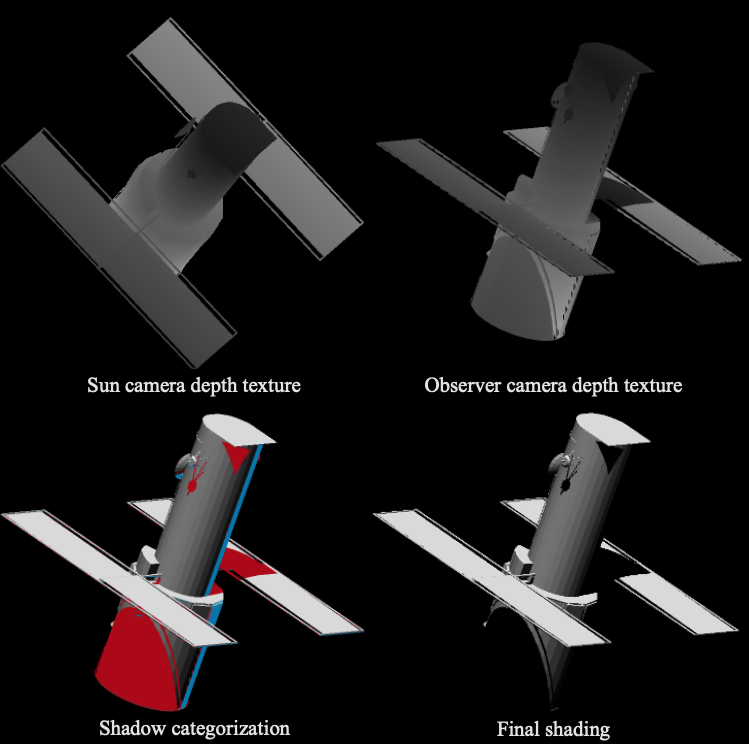
\includegraphics[width=\figmed]{hst_shadow_mapping/hst_shadow_mapping.png}
  \caption{Hubble Space Telescope shadow mapping with self (red) and horizon (blue) shadows rendered. Models from \cite{nasa_models}}
  \label{fig:hst_shadows_map}
\end{figure}

\subsection{Sampling Noisy Light Curves}

Given the irradiance of the object observed by the telescope, the noisy light curve is computed by building a grid containing the object signal, background noise, and sensor noise. On a pixel-by-pixel basis, the mean object signal is given by an alteration of Eq \ref{eq:airy_gaussian}:

\begin{equation} \label{eq:obj_signal_grid}
  C_{obj}(x, y) = \frac{0.838 \bar{C}_{all}}{2 \pi \sigma^2} \exp\left( - \frac{(x - x_0)^2 + (y - y_0)^2}{2 \sigma^2  s_{pix}^2} \right).
\end{equation}

In Eq \ref{eq:obj_signal_grid}, $\left(x_0, y_0\right)$ are the exact pixel coordinates of the object centroid, $\sigma$ is the Gaussian standard deviation from Eq \ref{eq:airy_variance} in arcseconds, and $s_{pix}$ is the pixel scale in arcseconds per pixel. Likewise, the total noise sampled in each pixel is given by samples from all the relevant source distributions:

\begin{equation} \label{eq:noise_signal_grid}
  C_{noise}(x, y) = N_{background} + N_{dark} + N_{trunc} + N_{read}.
\end{equation}

In Eq \ref{eq:noise_signal_grid}, $N_{background}$ is a sample drawn from $\mathrm{Pois}(\lambda_{background})$, $N_{dark}$ is drawn from $\mathrm{Pois}(\Delta t \lambda_{dark})$, $N_{trunc}$ is drawn from $\mathrm{Uniform}(-g/2, g/2)$, and $N_{read}$ is drawn from $\mathrm{Normal}(0, \sigma_{read}^2)$. 
\ProvidesFile{ch-light-curve-inversion.tex}[Light Curve Shape Inversion]
\graphicspath{{/Users/liamrobinson/Documents/msthesis/static_images/aas_2022_figs}}
\chapter{Light Curve Shape Inversion}

\section{Direct Inversion}

Traditionally, direct light curve inversion involves two distinct steps: a linear least squares problem to fit an EGI to the measured light curve, and a second optimization to produce accurate vertex positions and face adjacency information \cite{fan2020thesis}. The first step uses data-driven estimation to yield a valid and accurate EGI through a linear optimization. The second step is highly nonlinear and scales badly with facet count and geometric asymmetry, as discussed by Fan in \cite{fan2019}.

\subsection{The Extended Gaussian Image} \label{sec:egi_definition}

The discrete EGI $\vec{E} \in \mathbb{R}^{m \times 3}$ is composed of $m$ unit vectors $\hat{n}$ each scaled a nonnegative scalar $a \in \mathbb{R}, \: a_i \geq 0$ \cite{little1983}.

\begin{equation}
  \vec{E}_i = a_i \hat{n}_i
\end{equation}

In the context of shape inversion, the $m$ vectors $\hat{n}$ should be a relatively uniform tessellation of the unit sphere. A convex polytope can be uniquely represented by an EGI of facet normal vectors scaled by each facet's area. The set of normal vectors in an EGI is denoted $\mathcal{N}$ with the set of areas denoted $\mathcal{A}$. The vector of facet areas is denoted $\vec{a} \in \mathbb{R}^{m \times 1}$. The norm of the EGI is nottated $\| \vec{E} \| = \vec{a}$ with the `size' of the EGI $\|\vec{E}\| = m$.

The solution to the Minkowski problem proves the existence and uniqueness of a convex polytope for an EGI that satisfies the closure condition in Eq. \ref{egi_closure} \cite{minkowski1909}. Equivalently, an EGI uniquely represents a closed, convex polyhedron --- a polytope --- with no open boundaries, up to a translation.

\begin{equation} \label{egi_closure}
  \sum_{i=1}^m a_i \hat{n}_i = [0, 0, 0]
\end{equation}

While a given EGI uniquely represents a polytope, it is shared by an infinite number of non-convex and open geometries. An example of this extended family is depicted in Figure \ref{fig:egi_family} where larger circles indicate greater relative areas assigned to a given normal vector.

\begin{figure}[!htb]
  \centering
  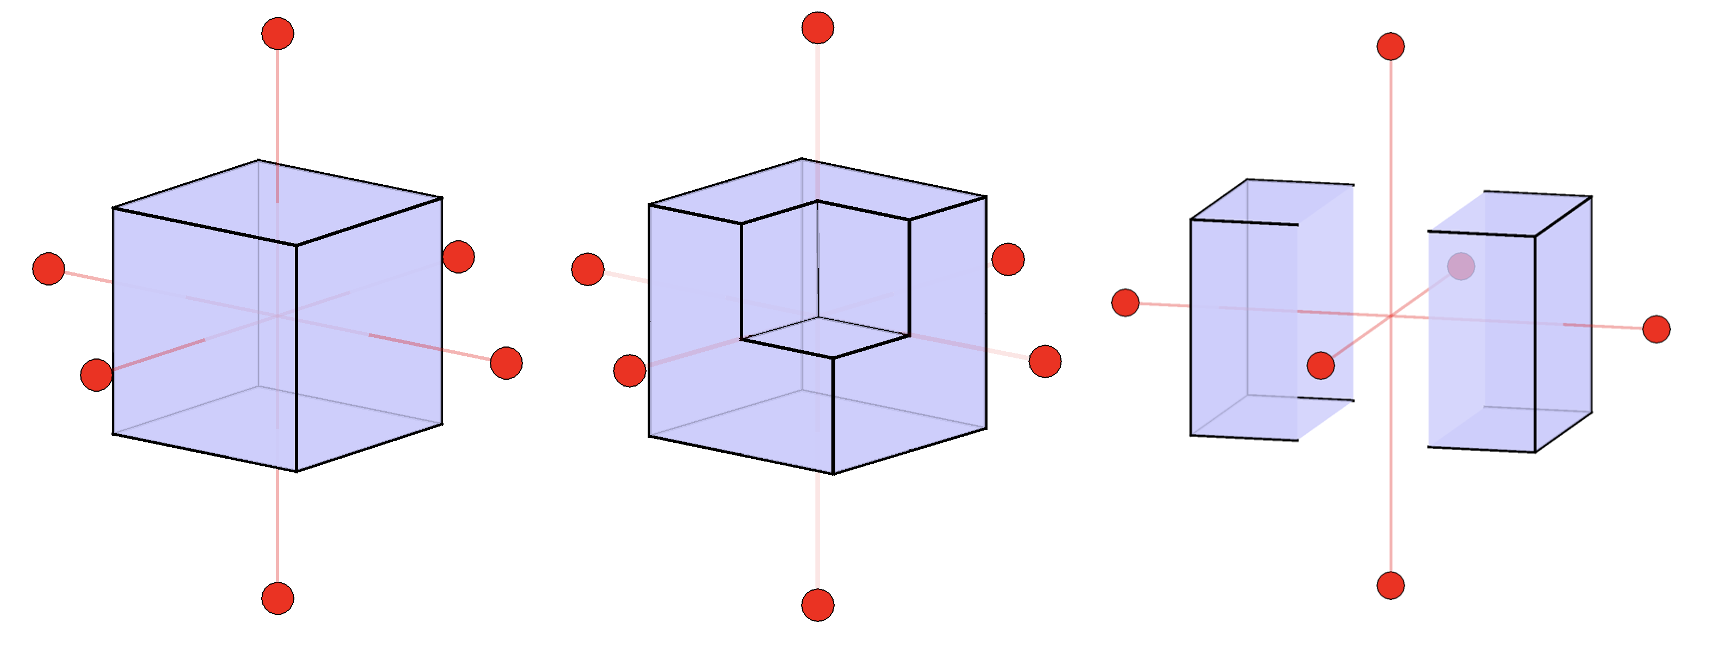
\includegraphics[width=\figmed]{convex_non_open_egis.png}
  \caption{Simplified convex, non-convex, and open EGI nonuniqueness}
  \label{fig:egi_family}
\end{figure}

\subsection{EGI Optimization}

The EGI fulfills two important criteria when applied to light curve inversion: it can be estimated directly from the light curve, attitude profile, and material properties, and uniquely represents a convex object \cite{kaasalainen2001}. Furthermore, convex geometry can be reconstructed from the EGI and vice versa through the dual transform \cite{little1985} and the Minkowski problem \cite{minkowski1909}. 

Once a light curve is obtained, direct shape inversion schemes sample $m$ candidate normal vectors $\hat{n}$ on the unit sphere to fit an EGI to the observed light curve $\vec{L}_\textrm{ref} \in \mathbb{R}^{n \times 1}$ \cite{friedman2020, fan2020thesis}. This is accomplished by solving an optimization problem to distribute the area vector $\vec{a}$ across the sampled normals to minimize the residual between the observed and modeled light curves. In practice, this is a constrained nonnegative least squares problem and can be solved efficiently for large numbers of normal vectors and light curve data points:

\begin{equation} \label{area_opt_convex}
  \min_{a}{\|\vec{L}_{\textrm{ref}} - G \vec{a}\|_2} \:\:\: \textrm{ subject to } \vec{a}_i \geq 0, \: \sum_{i = 1}^{m} \vec{a}_i \hat{n}_i = [0, 0, 0].
\end{equation}

It is important to note that the area estimated with Eq. \ref{area_opt_convex} is necessarily \textit{albedo-area} due to the diffuse reflectivity coefficient $C_d$ in Eq. \ref{lc_func_diffuse}. If the value of $C_d$ is uniform but unknown, the recovered geometry will incorrectly scaled without impacting the face adjacency or relative feature sizes.

The convex reflection matrix $G \in \mathbb{R}^{n \times m}$ with $ij$th entries $[g]_{ij}$ defined at time $i$ for each facet $j$ is defined as the normalized received facet irradiance per unit facet area:

\begin{equation} \label{ref_cond_matrix}
  [g]_{ij} = \frac{I_{ij}}{I_\textrm{Sun} a_j}.
\end{equation}

This relationship between the object irradiance and area defines the normalized convex light curve $\vec{L}_{\textrm{convex}}$, that produced by a convex object of facet areas $\vec{a}$ under the attitude profile and lighting conditions that yield $G$.

\begin{equation} \label{convex_lc_with_g}
  \vec{L}_{\textrm{convex}} = G \vec{a}
\end{equation}

The optimization in Eq. \ref{area_opt_convex} produces a coarse approximation of the true EGI as $m$ is finite. Increasing $m$ necessarily improves the quality and sparsity of the estimated EGI, but at the cost of computational resources. The estimation was performed using a synthetic light curve input from $n=500$ Sun and observer vectors uniformly sampled on the sphere in the body frame, producing a full rank $G$ matrix. $m = 500$ candidate normal vectors were sampled using a spherical Fibbonaci mapping described by Keinert et al. in \cite{keinert2015}. Results are visualized for an icosahedron in the body frame in Figure \ref{initial_ico_resampling}. Reconstructing the object at this stage is difficult due to the quantity of faces present in the estimated EGI. 

\begin{figure}[!htb]
  \centering
  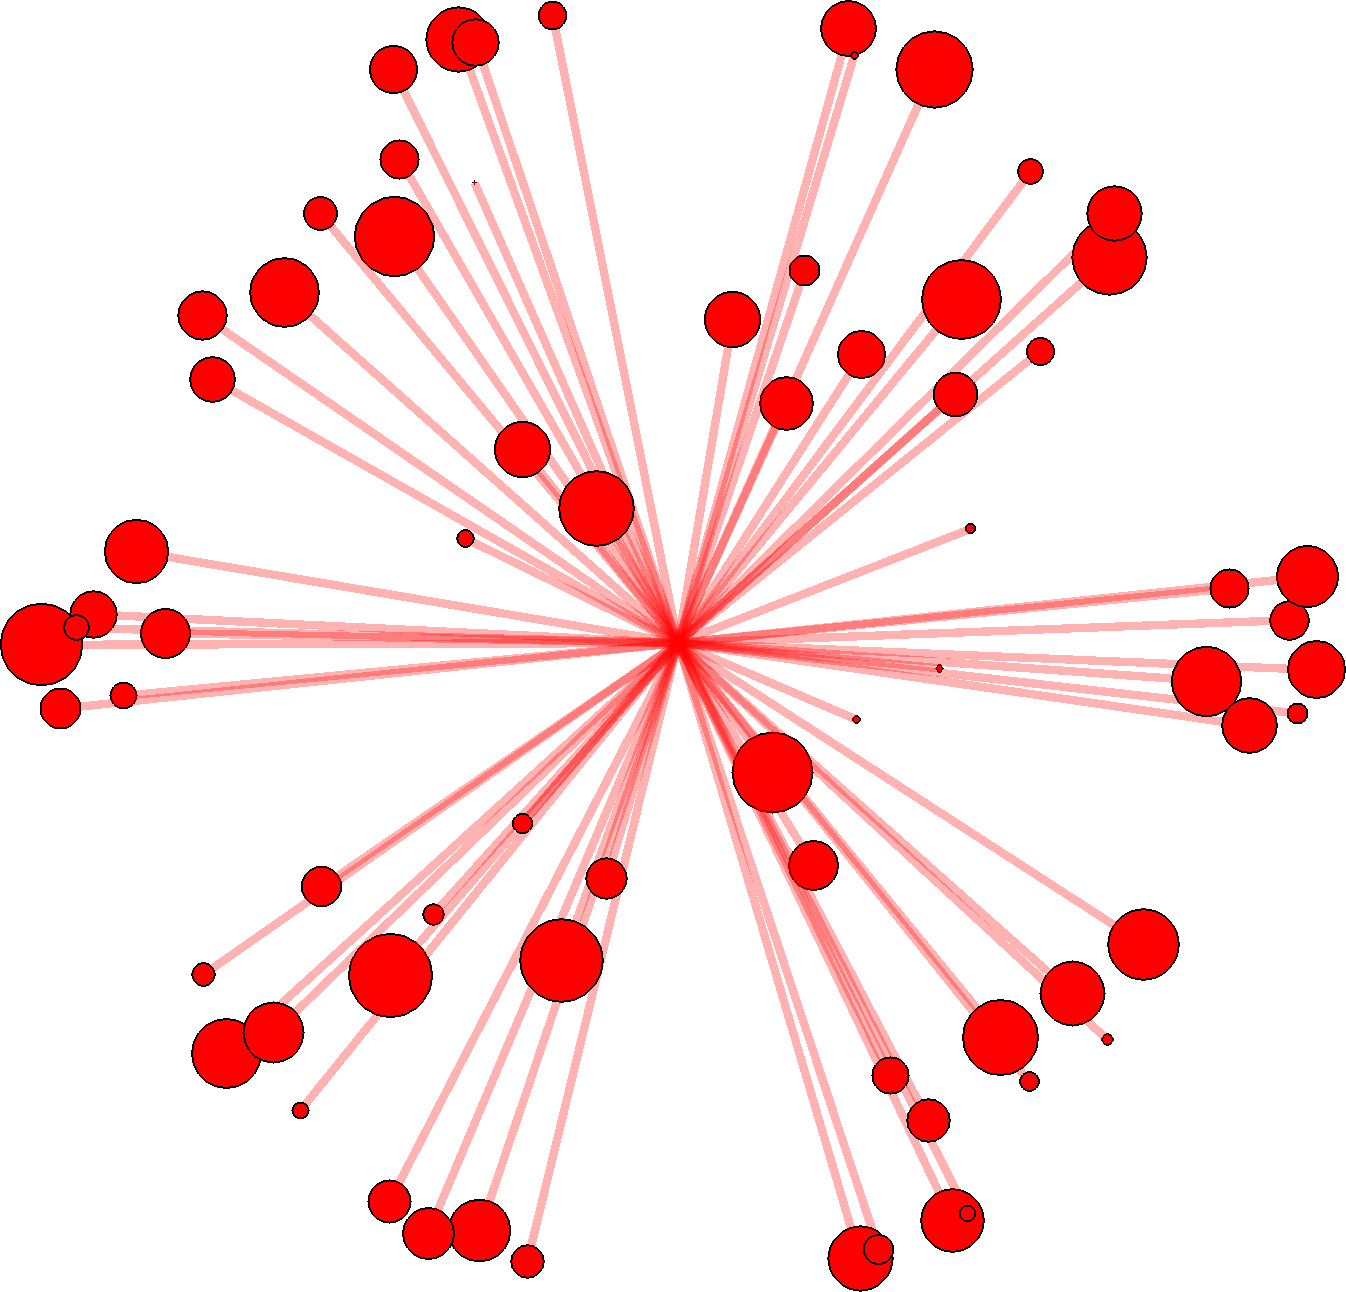
\includegraphics[width=150px]{ico_initial_egi.png}
  \caption{Initial icosahedron EGI optimization before resampling}
  \label{initial_ico_resampling}
\end{figure}

\subsection{EGI Resampling}

We propose a normal vector resampling step to promote a more accurate and sparse EGI. The normal vectors used in Eq. \ref{initial_ico_resampling} are generally correct, with each group clustering around a normal vector of the truth geometry. This clustering behavior occurs when none of the candidate normal vectors are sufficiently close to the truth. Resampling in a cone centered on each initial EGI normal vector provides more accurate candidates for EGI estimation. This process mimics a single optimization step with a much larger $m$, where the coarse EGI is used to exclude areas on the sphere with little or no normal area.

Uniformly sampling a cone of half-angle $\phi$ is accomplished by strategically sampling points on the unit sphere. 

\begin{equation} \label{cone_sample_n_pole}
  \hat{n}_{cone} = \begin{bmatrix}
    \sqrt{1-z^2}\cos{\theta} \\
    \sqrt{1-z^2}\sin{\theta} \\
    z \\
  \end{bmatrix}
\end{equation}

In Eq. \ref{cone_sample_n_pole} two coordinates are chosen $z \in [\cos{\phi}, 1]$ and $\theta \in [0, 2\pi)$, yielding a point uniformly distributed on a cone of half-angle $\phi$ about the central axis $[0, 0, 1]^T$ \cite{cone_sampling_wolfram}. These points are then rotated using a direction cosine matrix to center the cone on an axis of interest.

The number of new candidates sampled per initial solution vector and the cone half-angle should be adjusted on a case-by-case basis depending on the compute power available and light curve data quality.

Existing EGI optimization schemes like those of Fan \cite{fan2020thesis}, Friedman \cite{friedman2020}, and Cabrera \cite{cabrera2021} are limited by a single normal vector sampling step, leading to a lack of accuracy and sparsity in the optimized EGI. High-density normal vector sampling in regions known to contain non-zero area leads to EGI solutions that are generally more sparse and cluster more tightly about true normal vectors.

This process is shown in Figure \ref{resampled_ico_ns} for the same icosahedron with a half-angle $\phi = \frac{\pi}{20}$ and sampling density of $50$ candidate vectors per cone.

\begin{figure}[!htb]
  \centering
  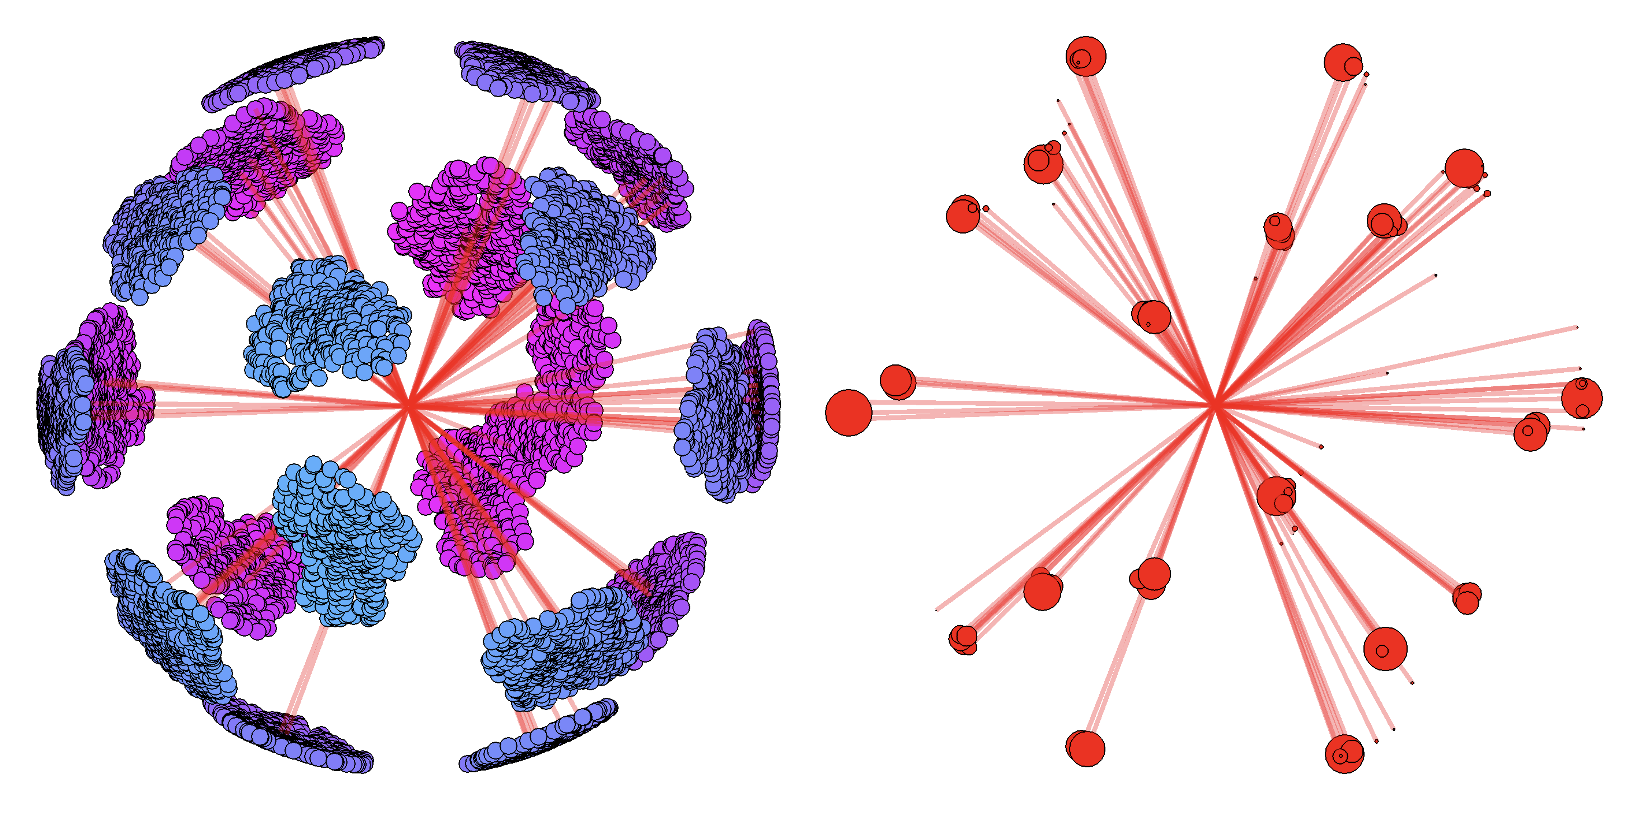
\includegraphics[width=350px]{ico_resampled_with_flower.png}
  \caption{Resampled normal vectors (left) with reoptimized EGI (right)}
  \label{resampled_ico_ns}
\end{figure}

\subsection{EGI Merging}

After resampling and reoptimizing with Eq. \ref{area_opt_convex}, the reestimated EGI is merged by computing all groups $\mathcal{G}$ of EGI vectors within an angular offset $\alpha$:

\begin{equation}
  \mathcal{G}_k = \left\{ \vec{E}_i \in \vec{E} \:\| \cos^{-1}\left( \frac{\hat{E}_i \cdot \hat{E}_k}{\|\vec{E}_i \| \| \vec{E}_k \|}\right) < \alpha \right\}.
\end{equation}

Groups are merged by summing all group members, yielding a single EGI vector $\vec{E}_m$ without loss of total area or closure. 

\begin{equation} \label{eq:fixing_egi}
  \vec{E}_m = \sum_{\vec{E} \in \mathcal{G}_k}{\vec{E}}
\end{equation}

In practice, the choice of $\alpha$ is dependent on the user's tolerance for discretization, as merging will approximate smooth geometry by discrete faces with normal vectors offset by $2\alpha$.

Merging the resampled EGI using Figure \ref{resampled_ico_ns} with $\alpha = \frac{\pi}{10}$ produces a final sparse EGI fit for object reconstruction, shown in Figure \ref{ico_merged_egi}. 

\begin{figure}[!htb]
  \centering
  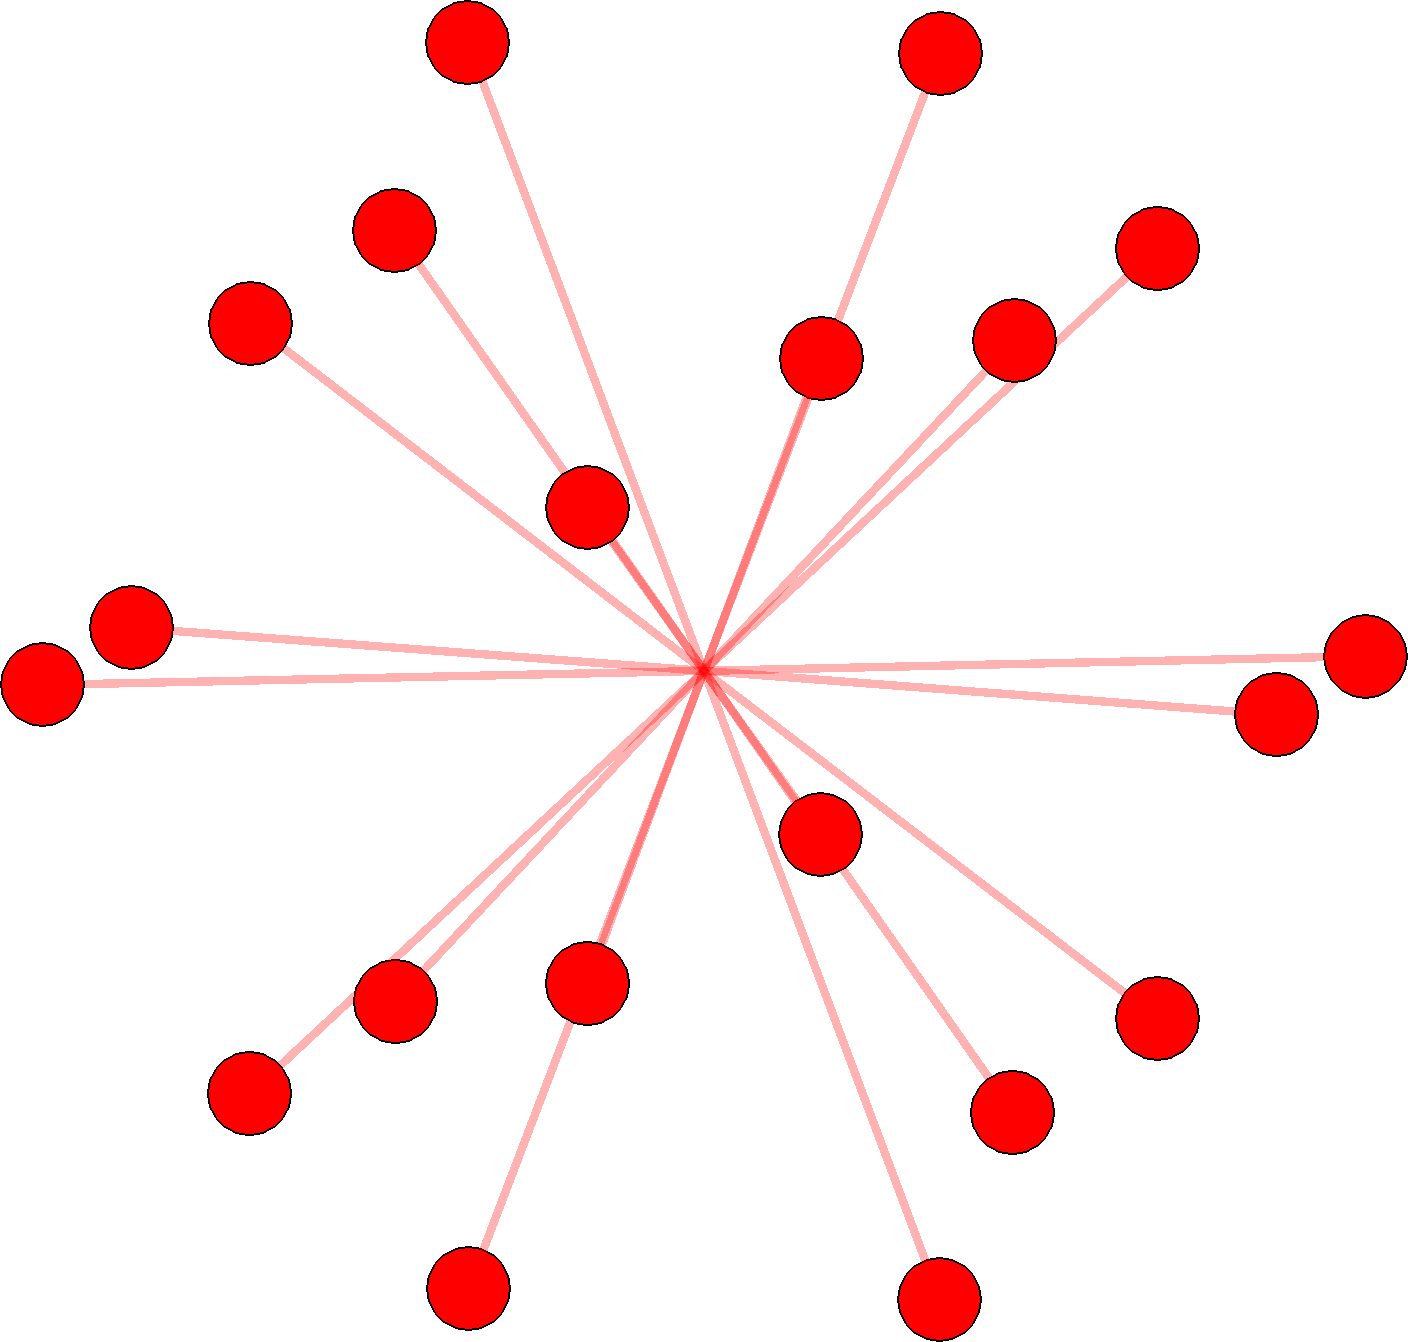
\includegraphics[width=150px]{ico_merged_egi.png}
  \caption{Merged icosahedron EGI}
  \label{ico_merged_egi}
\end{figure}

\subsection{Geometry Recovery from the EGI}

At this stage, the resampled and merged EGI represents a convex approximation of the underlying object with no guarantee of the closure of this EGI. The EGI closure constraint Eq. \ref{egi_closure} motivates a simple procedure to correct an invalid EGI by adding the mean closure error to each entry:

\begin{equation} \label{egi_validation}
  \vec{E}_{\textrm{closed}} = \vec{E}_{\textrm{open}} - \sum_{i=1}^m a_i \hat{n}_i .
\end{equation}

This step is not a novel contribution. Fan used a more complex optimization problem to adjust the EGI towards closure \cite{fan2020thesis}. This process is inproved with a simpler analytical correction. In practice, this process should be performed before each reconstruction to accelerate convergence. Failing to correct non-closed EGIs will cause convergence to a nonzero minimum in the reconstruction objective function as there is no corresponding convex object with the given EGI.

The unique convex object encoded by each closed EGI is reconstructed by solving for the polytope's set of vertices $\mathcal{V}$ and faces $\mathcal{F}$ encoding the adjacency relations between vertices. This is accomplished following the procedure introduced by Little in \cite{little1983} through the dual transformation. The dual set $\mathcal{D}$ are vertices in $(A, B, C) \in \mathbb{R}^3$ that satisfy the following plane condition for a point $(x, y, z)$ on each facet of the object:

\begin{equation} \label{dual_abc_form}
  Ax + By + Cz + 1 = 0
\end{equation}

If $(x, y, z)$ are chosen to be the closest points in the object's planes to the origin, the dual set $\mathcal{D}$ can be expressed in terms of the EGI and a support vector $\vec{h} \in \mathbb{R}^{\|F\| \times 1}$. The support vector is the perpendicular distance of each facet defining the object to the origin.

\begin{equation} \label{dual_egi_form}
  \mathcal{D} = \frac{\vec{E}}{ \| \vec{E} \| \vec{h}}
\end{equation}

The object's vertices $\vec{v}_{ref}$ are found by computing the convex hull of dual set vertices. Triplet of vertices on the resulting faces are used to find a single real vertex by intersecting the three planes defining the dual set vertices.

\begin{equation}
  \begin{bmatrix}
    v_{ref,x} \\
    v_{ref,Y} \\
    v_{ref,Z} \\
  \end{bmatrix} = \begin{bmatrix}
    v_{i,x} & v_{j,x} & v_{k,x} \\
    v_{i,y} & v_{j,y} & v_{k,y} \\
    v_{i,z} & v_{j,z} & v_{k,z}
  \end{bmatrix}^{-1} \begin{bmatrix}
    1 \\ 1 \\ 1
  \end{bmatrix}
\end{equation}

Convex face adjacency information is found by triangulating the convex hull of all reference vertices. The accuracy of the recovered geometry is entirely dependent on the correctness support vector $\vec{h}$ used to produce the dual set. Finding the true support vector is the challenge of the final optimization in convex shape inversion.

\subsection{Support Vector Optimization}

Prior work by Fan used Little's objective function for support vector optimization \cite{fan2020thesis,little1983}.

\begin{equation} \label{little_obj}
  f(\vec{h})_{\textrm{Little}} = \vec{h} \cdot \vec{a}
\end{equation} 

TODO: description of the optimization

\section{Non-Convex Feature Inversion}

\subsection{Non-Convex Feature Detection and Location}

Many human-made space objects are, as highlighted in Figure \ref{hst_bennu_shadows}, highly non-convex. As a result, their shape inversion is plagued by the fact that the Minkowski problem-driven reconstruction methods of Eq \ref{little_problem} cannot recover non-convex features. Instead of beginning from the ground up, the convex shape guess can be leveraged to detect and locate concavities.

We can retain information about large, unilateral object concavities during  EGI estimation in Eq. \ref{area_opt_convex} by relaxing the EGI closure constraint. This unconstrained form is also generally functional for most convex objects and can be used without loss of detail in the final reconstruction as long as closure correction in Eq. \ref{eq:fixing_egi} is still employed.

The mean axis of prominent concave features is determined by measuring the divergence of the optimized EGI from a closed object with the magnitude of the closure error $\vec{e}_{EGI}$.

\begin{equation} \label{eq:closure_error}
  \vec{e}_{EGI} = -\sum_{i=1}^{m} a_i \hat{n}_i.
\end{equation}

The EGI closure error vector in Eq \ref{eq:closure_error} represents the missing area on each body axis that could be added to close the object. The addition of the minus sign transforms the vector from expressing the presence of excess area to the absence of missing area. The closure error will be negligable if there are no concavities present. The closure error may also be negligable if there is no self-shadowing is present over the sampled attitude profile, therefore the closure error merely quantifies the self-shadowing that is occuring, not whether there may be self-shadowing in other orientations.

Under the strong assumption that the concavities present are major and unilateral, this EGI error vector points along the mean axis of the concavity.

TODO: replace this analytic relationship (which is bad and wrong) with an iteration to minimize LC error

\subsection{Concavity Creation}

Our process for creating an accurate concavity in the reconstructed convex guess proceeds in four major steps. The model is first subdivided to add more faces and vertices. Subdivided vertices are then classified by their proximity to the EGI error vector, indicating whether their positions should be updated. Boundary vertices are identified, and vertex positions are updated based on the estimated internal angle computed via Eq. \ref{eq:internal_angle_eq}.

\subsubsection{Model Subdivision}

Subdividing the initial convex object guess is essential for retaining object detail during concavity creation. A combination of linear subdivision, Loop subdivision, and remeshing algorithms are used to accomplish this. Linear subdivision is advantageous when object faces are equally sized and boundary edges must be maintained. Loop subdivision is preferable when there are numerous vertices so that subdivisions do not drastically diverge from the initial boundary surface. Loop subdivision softens sharp edges as it relies on B-splines to interpolate new vertex positions \cite{loop1987}. The specific type and resolution of subdivision used depends on the level of detail the user needs to maintain in the introduced concavity, although linear subdivision followed by Loop subdivision is a useful baseline. Varying combinations of subdivision are shown in Figure \ref{fig:subd_grid} to illustrate the available configurations.

\begin{figure}[!htb]
  \centering
  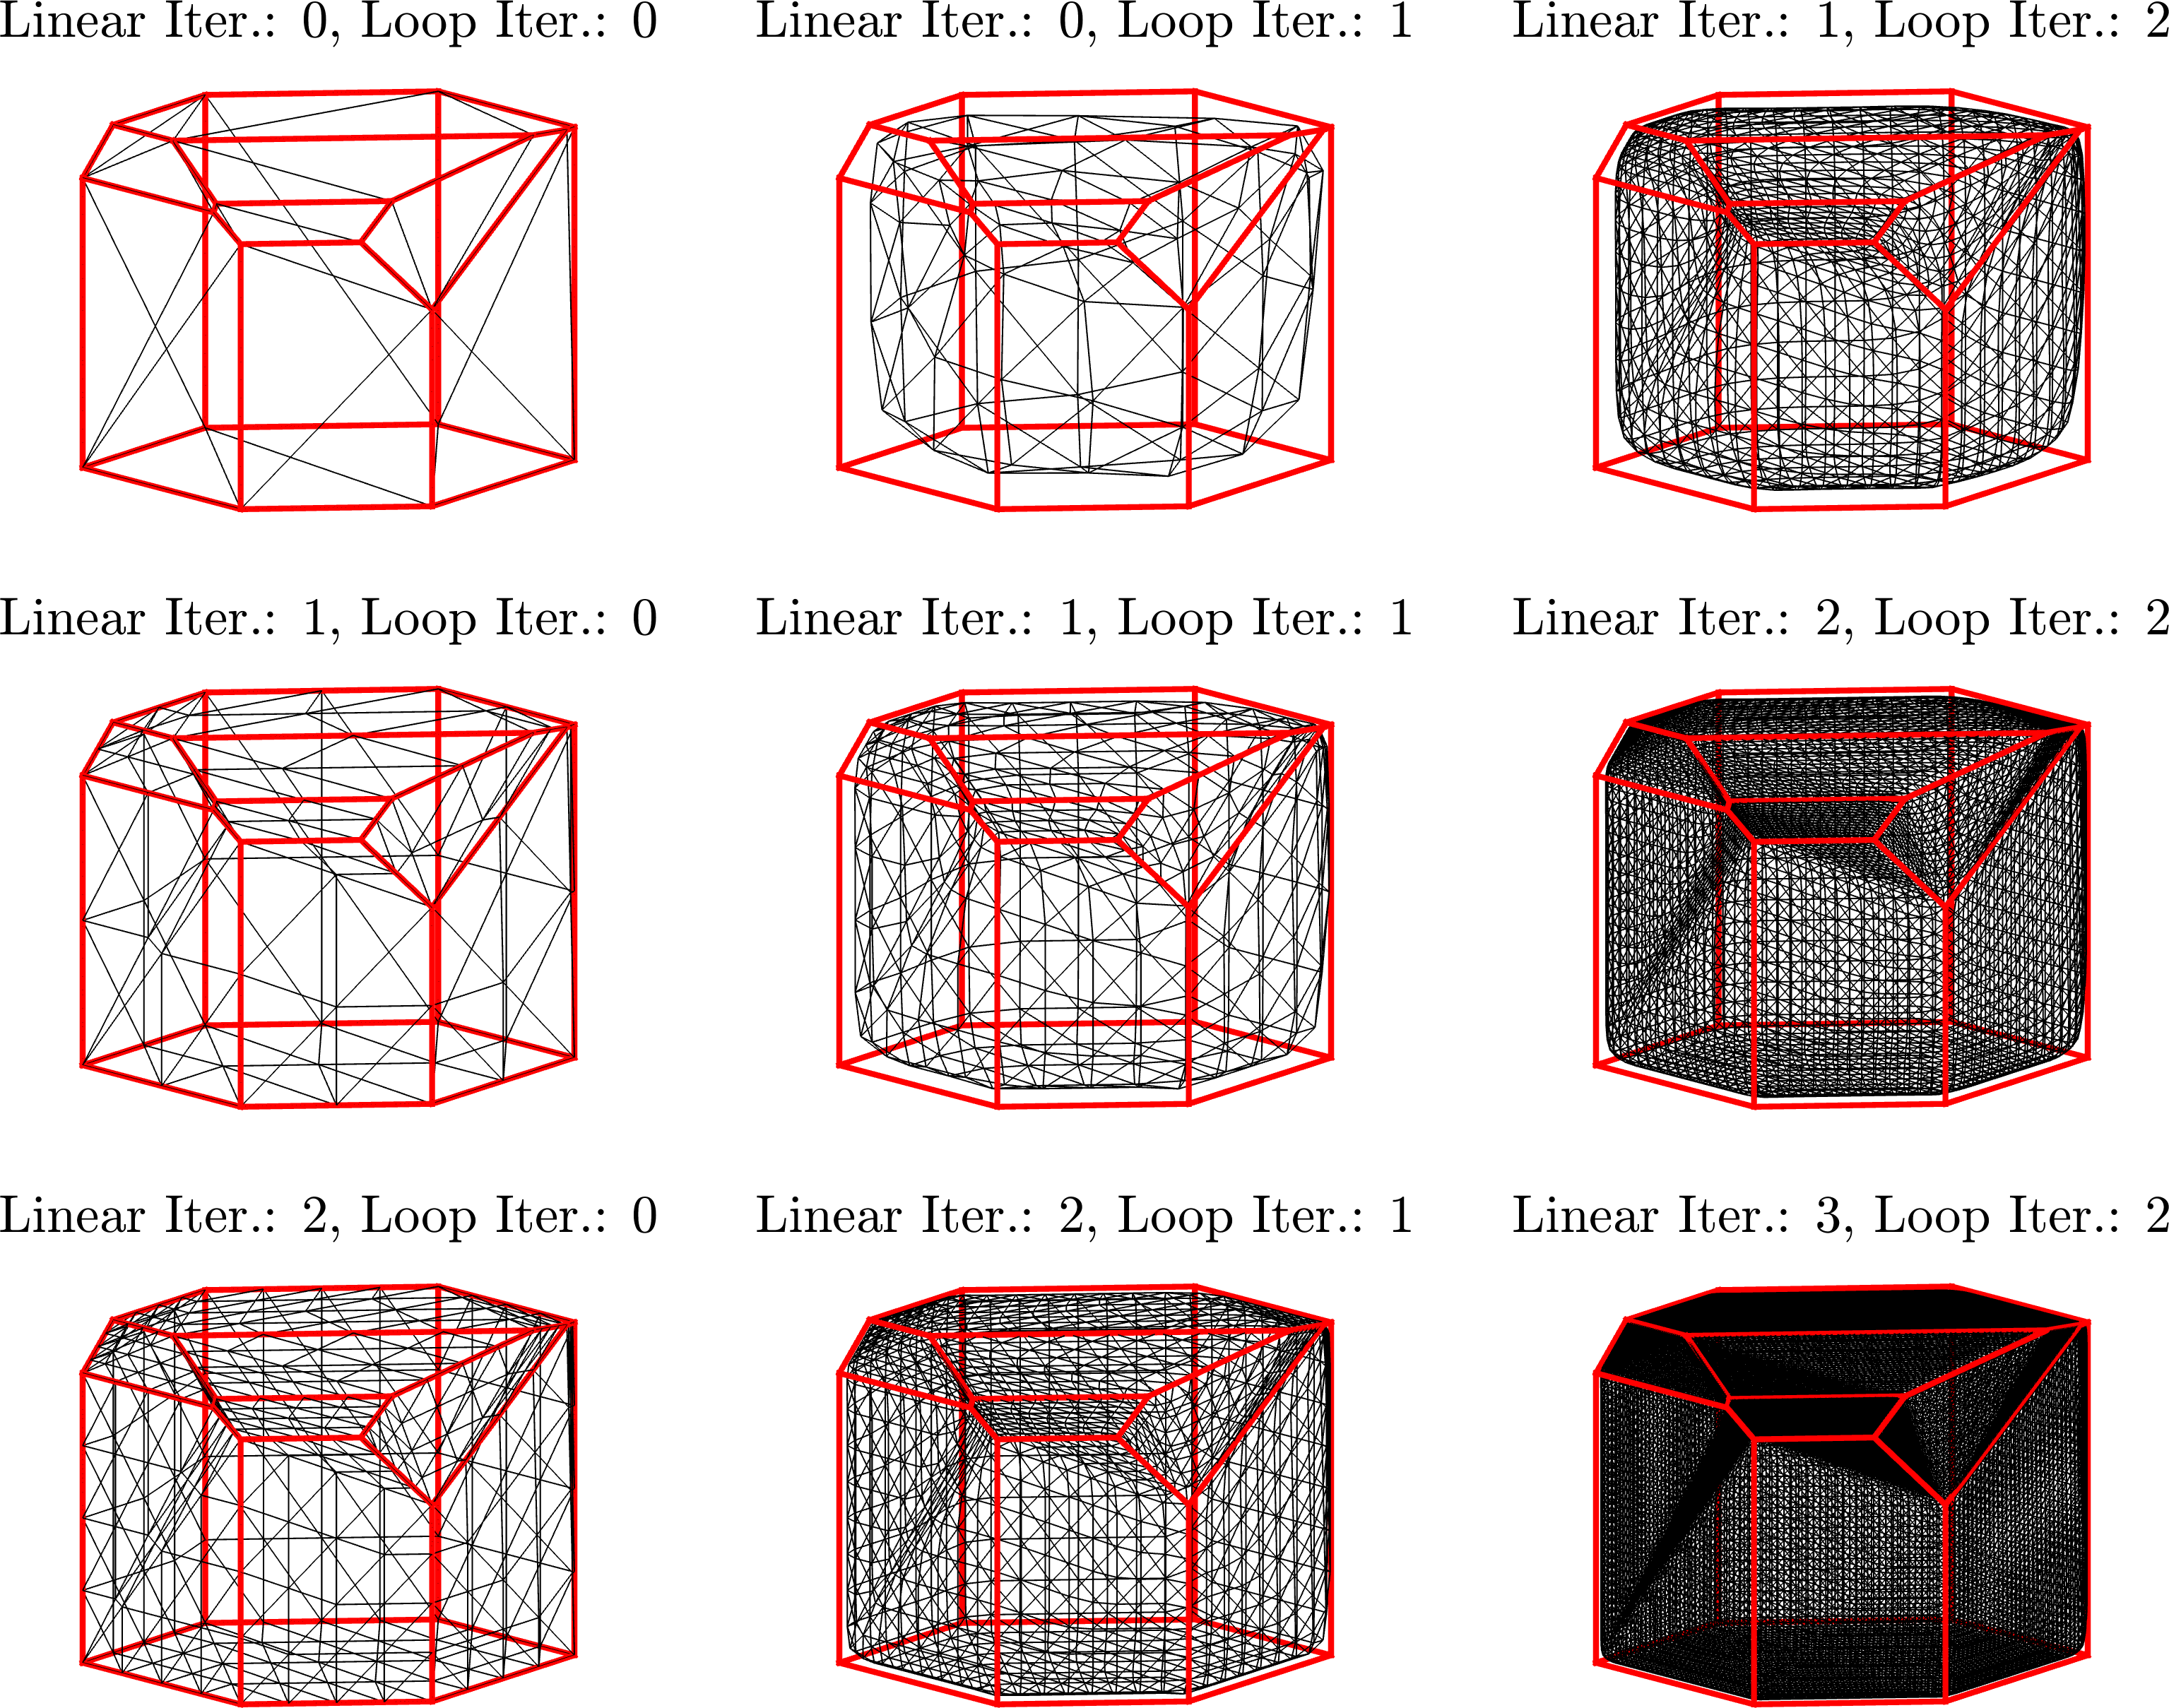
\includegraphics[width=350px]{subd_grid.png}
  \caption{Subdivided object (black) with reference (red) with various levels of subdivision}
  \label{fig:subd_grid}
\end{figure}

\subsubsection{Vertex Classification and Displacement}

When introducing a concavity, it is important to classify which vertices are part of the concave feature --- and therefore need to be updated --- and which vertices should remain unaffected. This is accomplished by measuring the angle from each face normal to the EGI error vector, where faces with normal vectors within an angle of $\pi/2$ to the error vector must be updated. In reality, all face normals and areas are impacted by the presence of the concavity in the area optimization Eq. \ref{area_opt_convex} and EGI correction step Eq. \ref{egi_validation}. Selecting the angle deflect $\pi/2$ updates all faces above the horizon from the EGI error vector. This bound tends to produce visually accurate concavities. Faces requiring an update are termed \textit{free} faces, with all others termed \textit{root} faces.

Vertices on free faces are further classified as being \textit{root-adjacent} or \textit{free}. Root-adjacent vertices are part of at least one root face, whereas free vertices belong to only free faces. Classifying vertices in this way results in a border of root-adjacent vertices around the interior free vertices, visualized in Figure \ref{fig:root_and_free}.

\begin{figure}[!htb]
  \centering
  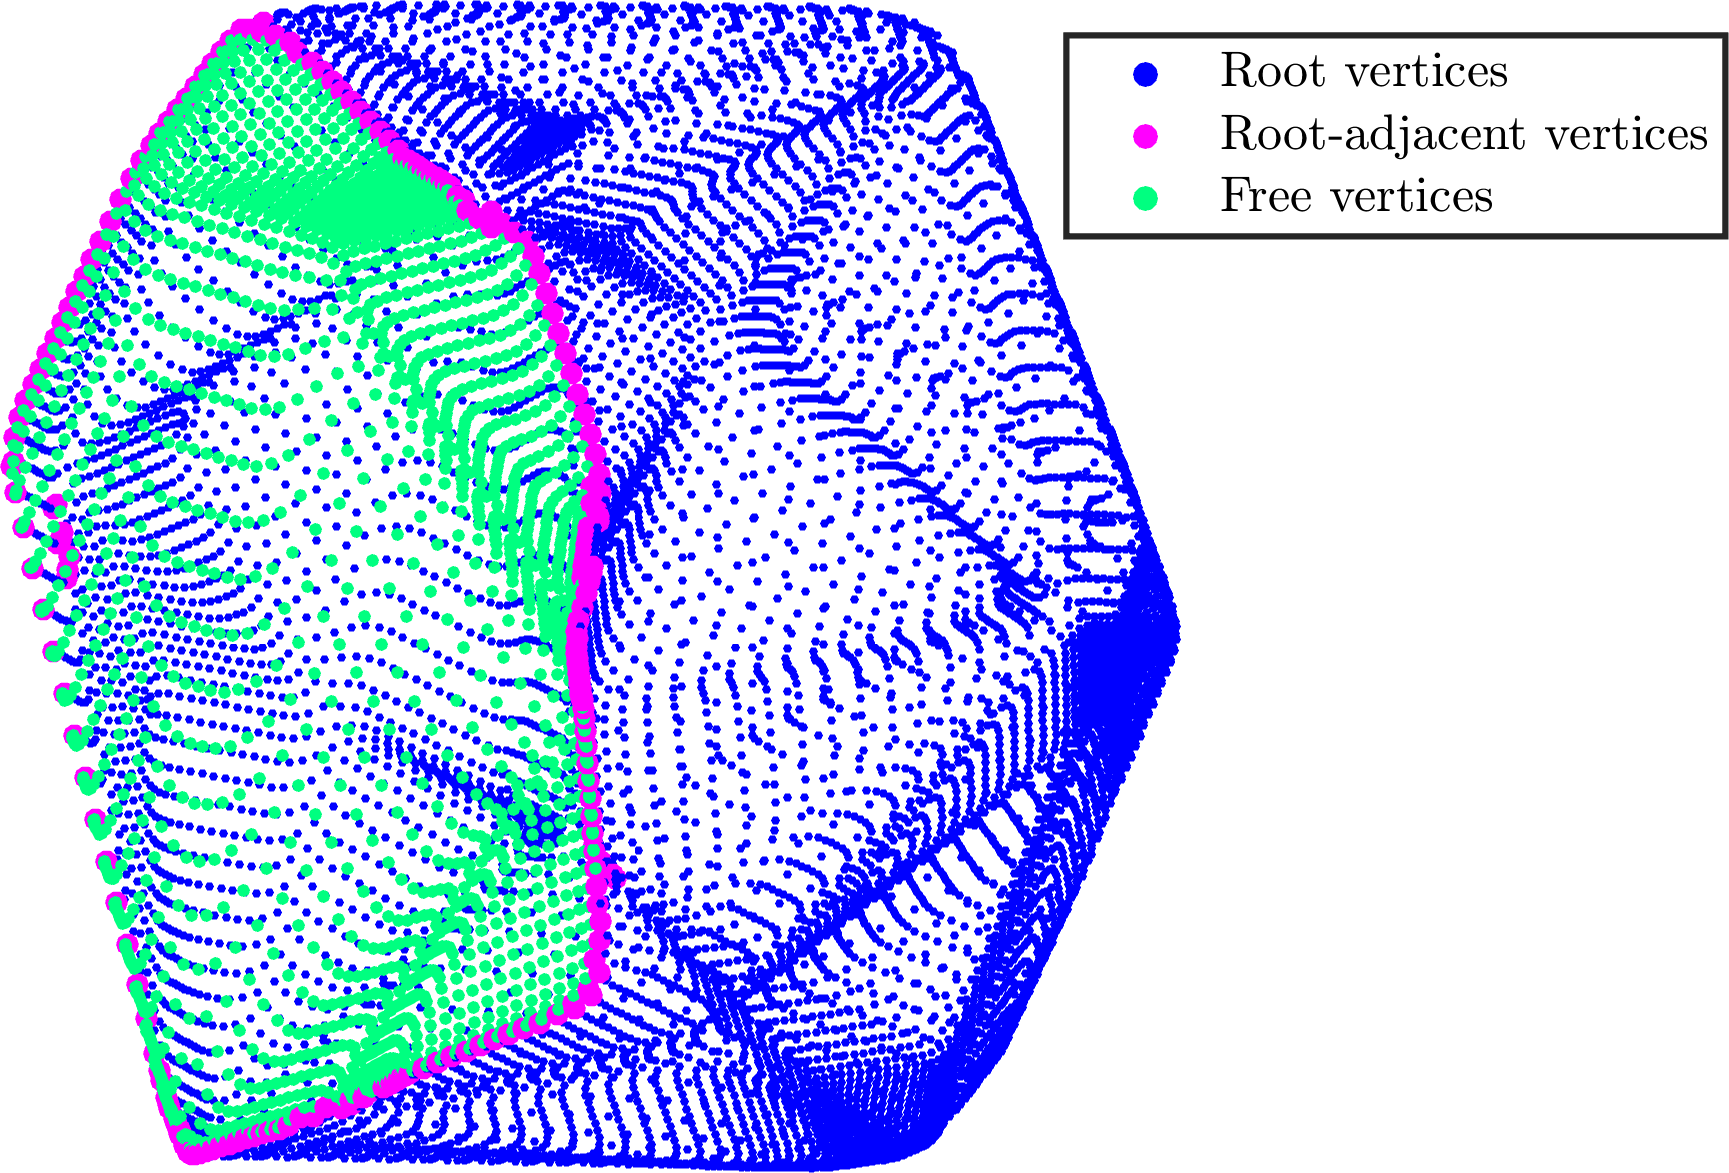
\includegraphics[width=250px]{rootadj_and_free_verts_try2.png}
  \caption{Root-adjacent and free vertices}
  \label{fig:root_and_free}
\end{figure}

Given the estimated internal angle $\psi_{est}$ and the error vector $\hat{e}_{EGI}$, each $i$th free vertex is displaced to introduce a geometrically accurate concavity by moving each a distance $d_i$ in the direction of $-\hat{e}_{EGI}$:

\begin{equation} \label{eq:flip_depth}
  d_i = p_i \sqrt{\csc^2 \frac{\psi_{est}}{2} - 1},
\end{equation}

where $p_i$ is the distance from each $i$th free vertex to the nearest root-adjacent vertex.

\section{Non-Convex Object Reconstruction Results}

Displacing free vertices in the EGI error vector direction by $d_i$ yields accurate concavities for objects whose concave boundaries lie in a plane. The result of applying this process to a set of representative convex objects is shown in Figure \ref{fig:non_convex_recon_of_non_convex} using the same attitude profiles and as in Figure \ref{convex_grid}. 

\begin{figure}[!htb]
  \centering
  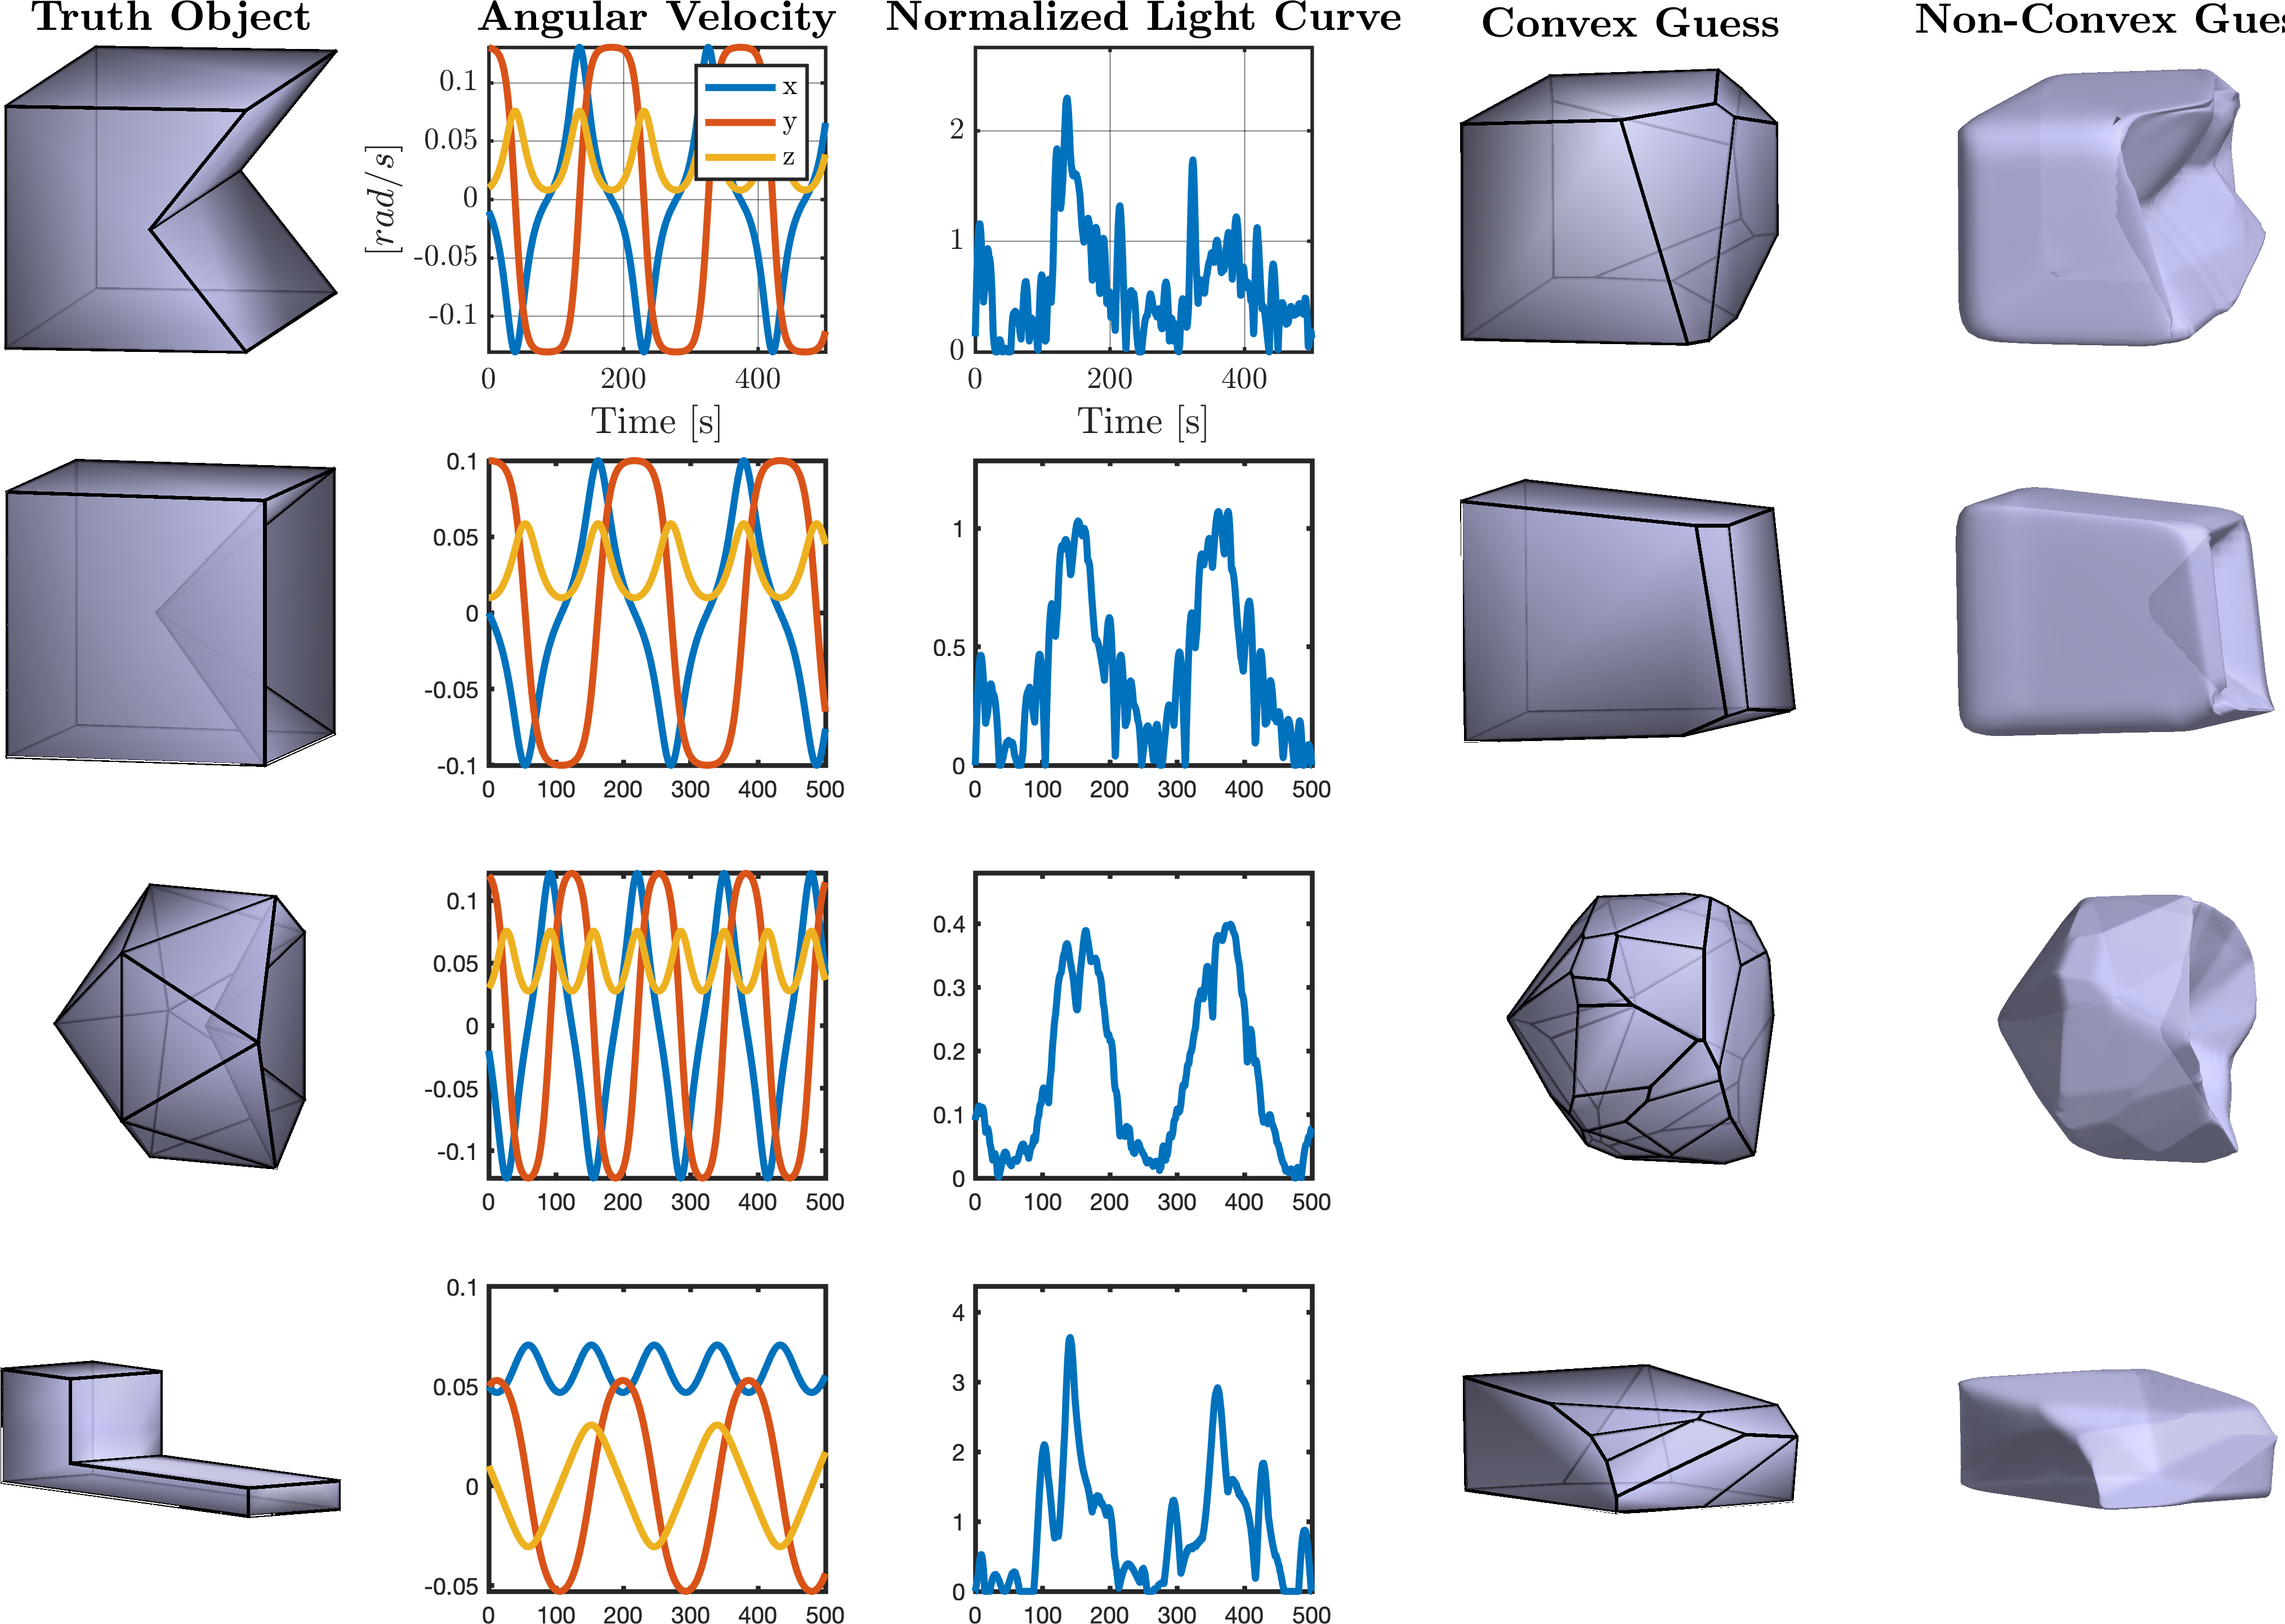
\includegraphics[width=400px]{rec_non_convex_objs/non_convex_grid_of_nonconvex_try2.png}
  \caption{Collapsed house, cube, icosahedron, and box-wing satellite reconstructions using vertex displacement}
  \label{fig:non_convex_recon_of_non_convex}
\end{figure}

The collapsed cube and icosahedron in Figure \ref{fig:non_convex_recon_of_non_convex} are recovered effectively, but the collapsed house and box-wing satellite expose two limitations of the vertex displacement technique. In the case of the house where the concavity boundary is not constrained to a plane, the edges of the created concave feature are incorrect. The box-wing satellite's shadowing geometry leads the convex guess to be a poor approximation of the geometry outside of the concavity while also inheriting the same problem as the house.

This vertex displacement scheme will negligibly impact the convex guess if the truth object is also convex. A convex truth object will produce a small $\|\vec{e}_{EGI}\|$, causing the vertex update depth $d_{i}$ to trend towards zero as the estimated internal angle approaches $\psi = 180^\circ$. This is illustrated in Figure \ref{fig:non_convex_recon_of_convex} using the same input convex objects and attitude profiles as in Figure \ref{convex_grid}.

\begin{figure}[!htb]
  \centering
  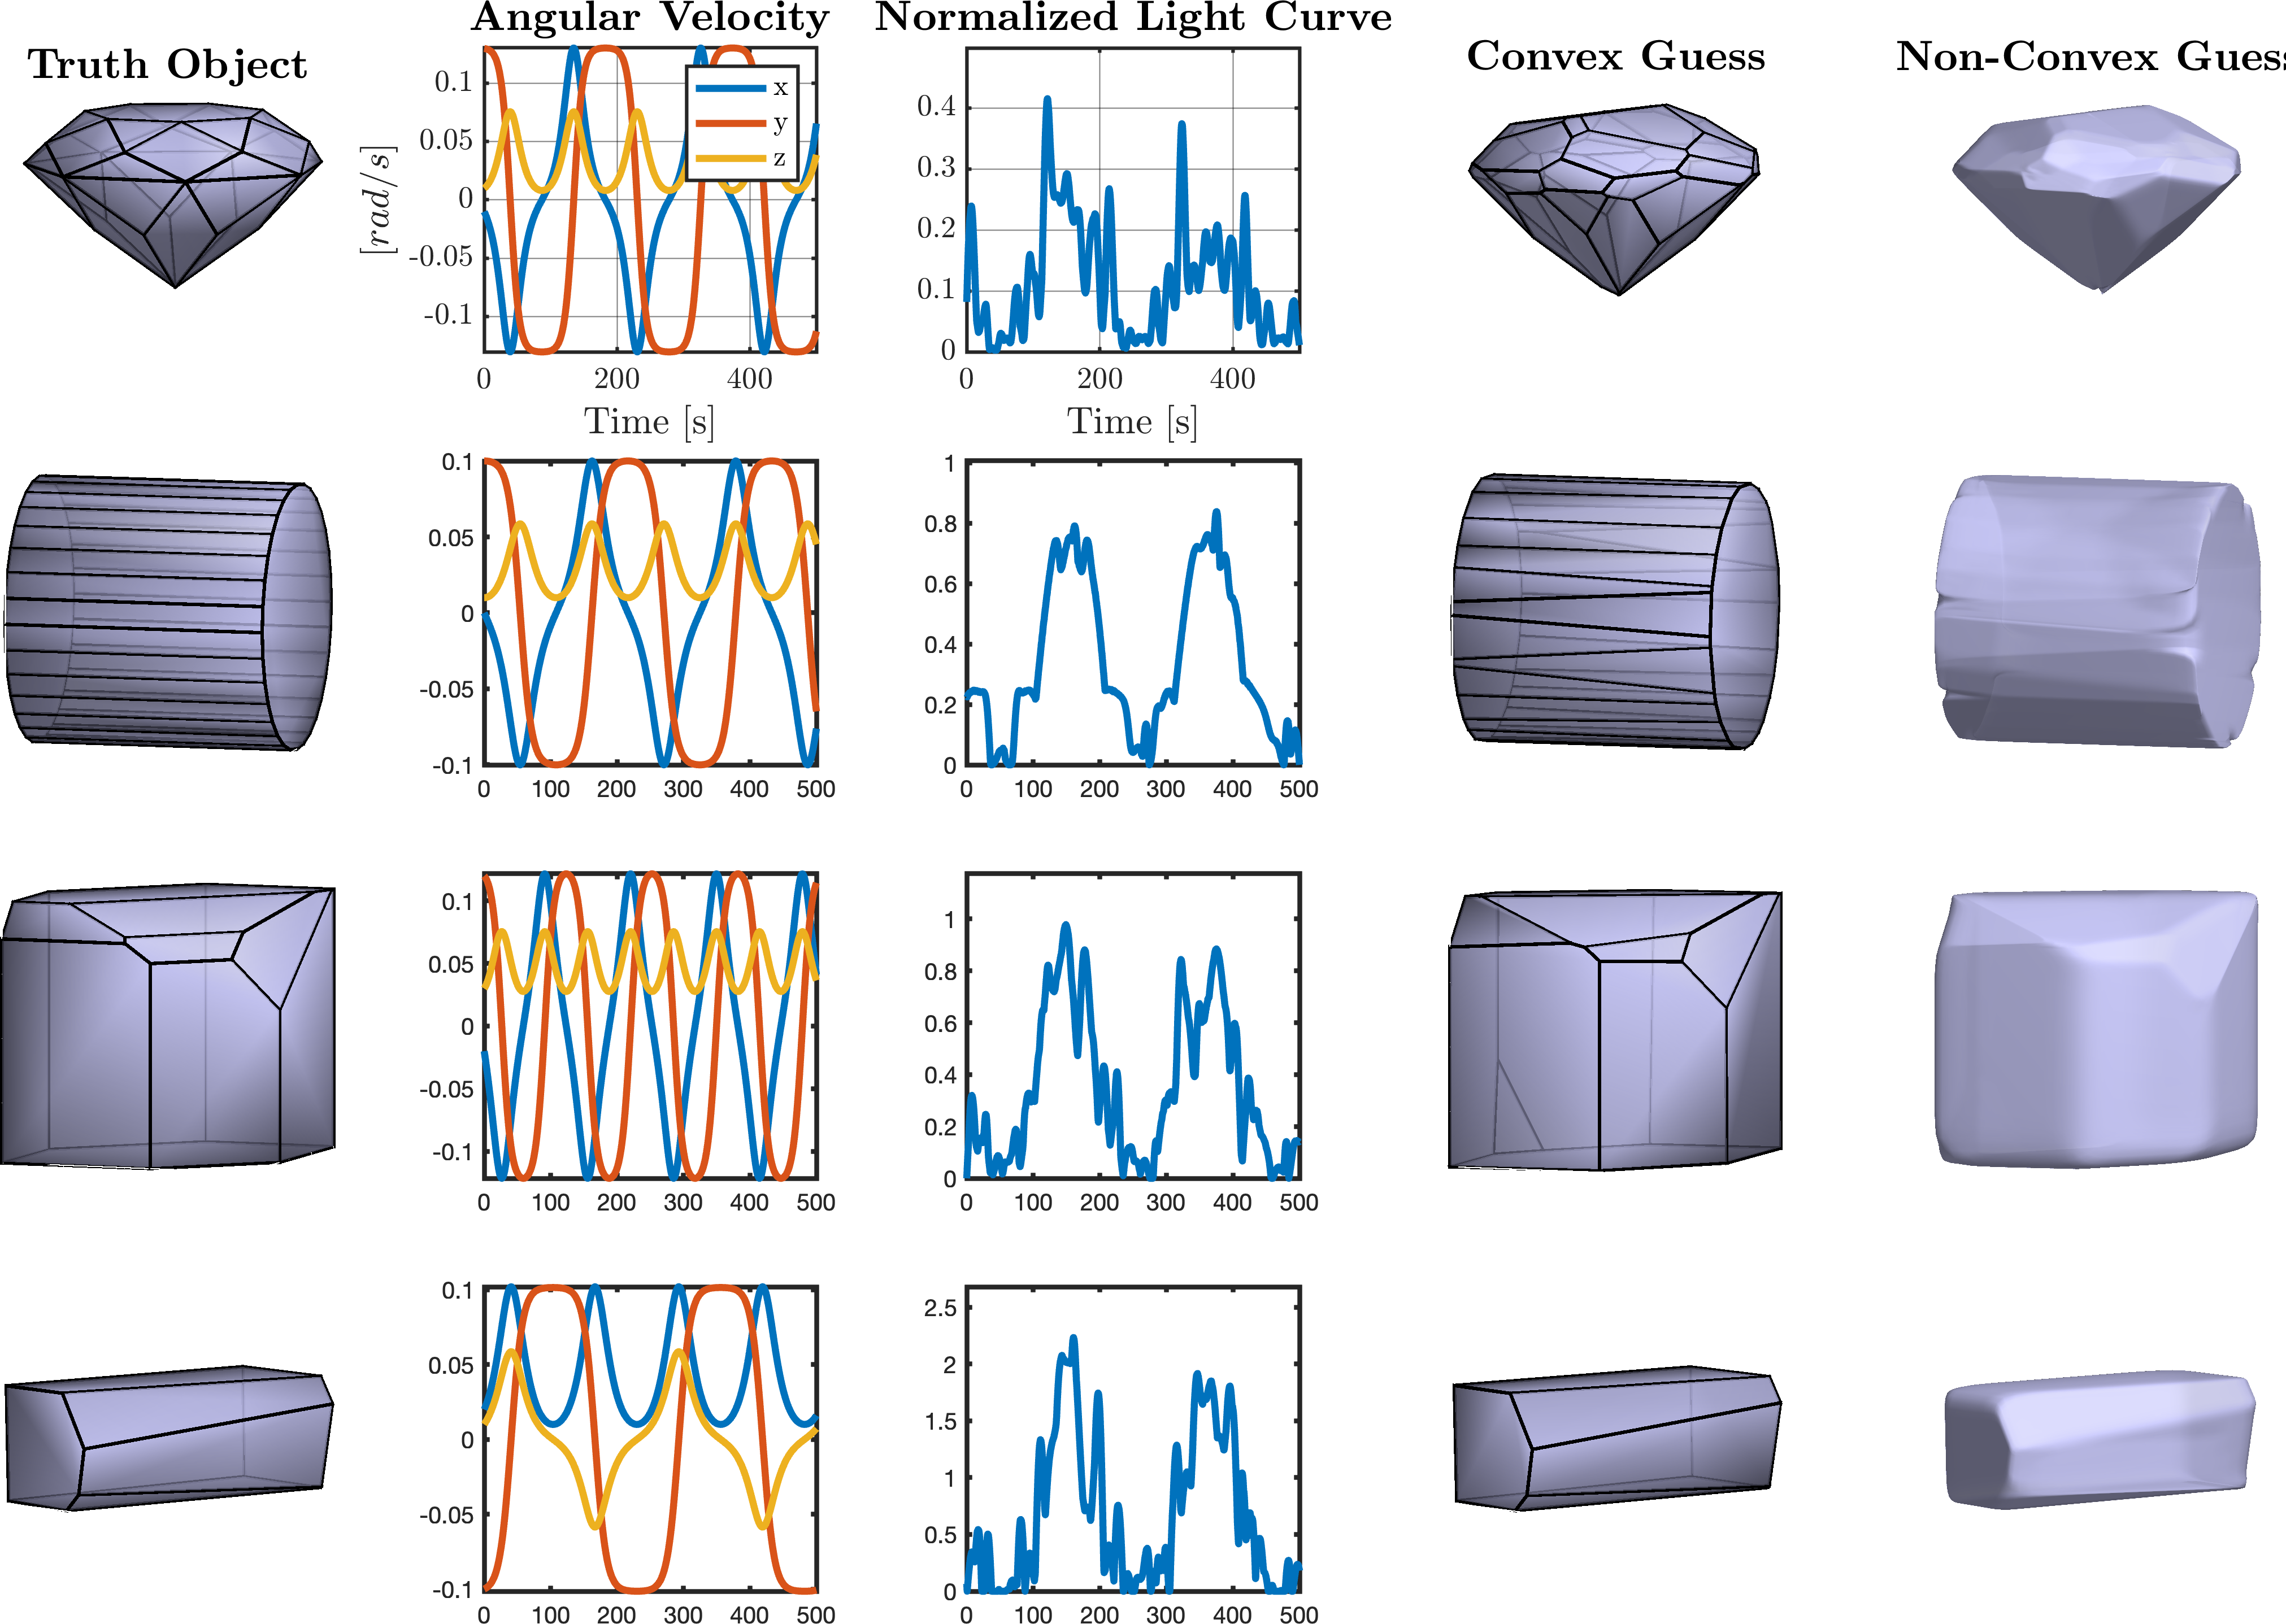
\includegraphics[width=400px]{rec_non_convex_objs/non_convex_grid_of_convex_try2.png}
  \caption{Convex objects under vertex displacement procedure}
  \label{fig:non_convex_recon_of_convex}
\end{figure}

Figure \ref{fig:non_convex_recon_of_convex} clearly displays the compatibility of vertex displacement with truly convex objects. All objects are reconstructed faithfully in both their convex and non-convex inversions, with the same caveats noted in the discussion following Figure \ref{convex_grid}. Some truly sharp edges are rounded during mesh subdivision as seen in the gem or rectangular prism. That said, others like the cylinder become more accurate as subdivision reintroduces continuity lost to discretization in EGI merging.


%%% RESULTS

%%% CONCLUSION
\ProvidesFile{ch-recommendations.tex}[2022-10-05 recommedations chapter]

\chapter{RECOMMENDATIONS}

Buy low.
Sell high.

\ProvidesFile{ch-future-work.tex}[Future Work]
\chapter{Future Work}
\ProvidesFile{ch-appendices.tex}[Appendices]
\chapter{Appendices}

\section{Shadow Mapping} \label{data:shadow_mapping}

\subsection{Shading} \label{data:shading}

\begin{algorithm}
  \caption{Pixel-wise shading algorithm with shadow mapping}\label{alg:pix_shading}
  \begin{algorithmic}
    \State $L \in \mathbb{S}^2$ \Comment{Unit vector from object origin towards Sun}
    \State $O \in \mathbb{S}^2$ \Comment{Unit vector from object origin towards observer}
    \State $N \in \mathbb{S}^2$ \Comment{Outward-pointing surface normal vector at pixel coordinates}
    \State $(C_d, C_s, n) \in \mathbb{S}^2$ \Comment{Reflection coefficients and exponent for the BRDF}
    \Require $C_d + C_s \leq 1$ \Comment{Enforce energy conservation}
    \State $MVP_{Sun} \in \mathbb{R}^{4 \times 4}$ \Comment{MVP matrix for the Sun camera}
    \State $(x, y) \in \mathbb{Z}^2$ \Comment{Integer pixel coordinates from the observer camera}
    \State $R_{pix,obs} \in \mathbb{R}^3$ \Comment{World coordinates of the pixel; provided by OpenGL}
    \State $\left[(x_{homo,Sun}, y_{homo,Sun}, ...\right] \gets MVP_{Sun} \left[ R_{pix,obs}, 1 \right]^T$
    \State $x_{Sun} \gets \left(1 + p_{x, homo}\right) \frac{w_\mathrm{pix}}{2} $ \Comment{Homogeneous coordinates from the Sun camera}
    \State $y_{Sun} \gets \left(1 + p_{y, homo}\right) \frac{a \cdot w_\mathrm{pix}}{2} $
    \State $D_{Sun} \gets  d(x_{sun}, y_{sun})$ \Comment{Closest pixel depth to the Sun direction}
    \State $D_\mathrm{obs} \gets \left( L - O \right) \cdot L$ \Comment{Closest pixel depth in the Observer direction}
    \If{$D_\mathrm{obs} > D_{Sun}$}
      \State $\delta_{ss} = 1$ \Comment{Pixel is self-shadowed}
    \Else 
      \State $\delta_{ss} = 0$ \Comment{Pixel may be illuminated}
    \EndIf
    \If{$\left(N \cdot L\right) > 0 \textrm{ and } \left(N \cdot O\right) > 0$}
      \State $f_r(\vctr{x}, L, O) = 0$ \Comment{Pixel cannot be both observed and illuminated}
    \Else 
      \State $f_r(\vctr{x}, L, O) = \mathrm{Phong}(L, O, N, C_d, C_s, n)$ \Comment{The pixel is shaded with the BRDF}
    \EndIf
    \State $\mathrm{IM}(x, y) = f_r(\vctr{x}, L, O) \left(N \cdot L\right) $ \Comment{Image pixel value}
  \end{algorithmic}
\end{algorithm}

\clearpage
\section{Astronomical Spectra Data} \label{data:spectra}

\subsubsection{Atmospheric Extinction} \label{data:atm} Data from \cite{krag2003}.
The atmospheric extinction coefficient is dimensionless.
\begin{listing}[H]
\inputminted[breaklines=true, breakanywhere=true, breaksymbol=\hspace{0pt}, fontsize=\footnotesize]{json}{/Users/liamrobinson/Documents/PyLightCurves/mirage/resources/data/atmos_extinction.json}
\end{listing}

% \subsubsection{Quantum Efficiency} \label{data:qe}
% The quantum efficiency spectrum has units $\left[ \frac{e^-}{m} \right]$.
% \begin{listing}[H]
% \inputminted[breaklines=true, breakanywhere=true, breaksymbol=\hspace{0pt}, fontsize=\footnotesize]{json}{/Users/liamrobinson/Documents/PyLightCurves/mirage/resources/data/kaf16803_quantum_efficiency.dat}
% \end{listing}

\subsection{Lunar Phase Factor}
The lunar phase factor is a function of the phase angle in radians and is dimensionless. Data from \cite{daniels1977}.
\begin{listing}[H]
\inputminted[breaklines=true, breakanywhere=true, breaksymbol=\hspace{0pt}, fontsize=\footnotesize]{json}{/Users/liamrobinson/Documents/PyLightCurves/mirage/resources/data/lunar_phase.json}
\end{listing}

\clearpage
\subsection{Scattered Moonlight}
The scattered moonlight radiance in $\left[ \frac{W}{sr \cdot m^2 \cdot m} \right]$ is a function of the difference in the line of sight and Moon azimuths \texttt{delta\_az} in radians, the zenith angle of the Moon \texttt{z\_moon} in radians, and the zenith angle of the line of sight \texttt{z\_obs} in radians. Data from \cite{daniels1977}.

\begin{listing}[H]
\inputminted[breaklines=true, breakanywhere=true, breaksymbol=\hspace{0pt}, fontsize=\footnotesize]{json}{/Users/liamrobinson/Documents/PyLightCurves/mirage/resources/data/moonlight.json}
\end{listing}

\clearpage
\subsection{Zodiacal Light} \label{data:roach_zod}

The zodiacal light surface brightness in $S_10$ is a function of the latitude \texttt{"ecliptic\_lat"} and longitude \texttt{"ecliptic\_lon"} of the line of sight in the solar system ecliptic reference frame, both expressed in radians. Data from \cite{roach1972}.

\begin{listing}[H]
\inputminted[breaklines=true, breakanywhere=true, breaksymbol=\hspace{0pt}, fontsize=\footnotesize]{json}{/Users/liamrobinson/Documents/PyLightCurves/mirage/resources/data/zodiacal.json}
\end{listing}

\clearpage
\section{Telescope Parameters}

\subsubsection{Purdue Optical Ground Station}

\begin{table}[ht]
    \centering
    \begin{tabular}{|l|l|}
    \hline
    \textbf{Parameter} & \textbf{Value} \\ \hline
    FWHM                & $1.5$                              \\ \hline
    Sensor dimensions    & $ 0.03690 \times 0.03690 \: [m]$                               \\ \hline
    $f$ number   & $7.2$                              \\ \hline
    Aperture diameter $D$       & $0.35560 \: [m]$                              \\ \hline
    Secondary diameter         & $0.1724660 \: [m]$                              \\ \hline
    Sensor pixels               & $4096 \times 4096$                              \\ \hline
    Pixel size               & $9.009 \cdot 10^{-6} \: [m / \textrm{pix}]$                              \\ \hline
    Pixel scale $s_\mathrm{pix}$              & $0.72545 \: [arcsec]$                              \\ \hline
    Field of view               & $0.824425^\circ \times 0.824425^\circ$                              \\ \hline
    Integration time $\Delta t$              & $10 \: [s]$                              \\ \hline
    Integration dark noise $\lambda_{dark}$ & $3 \: \left[ e^- / \mathrm{pix} / s\right]$ \\ \hline
    Read noise variance $\sigma_\mathrm{read}^2$ & $9 \: \left[ e^- \right]$ \\ \hline
    CCD gain $g$ & $1$ \\ \hline
    \end{tabular}
    \caption{Purdue Optical Ground Station telescope parameters}
    \label{tb:pogs_parameters}
  \end{table}

\clearpage
\section{Wavefront OBJ Example} \label{sec:obj_listing}

\begin{listing}[ht]
    \inputminted[breaklines=true, breakanywhere=true, breaksymbol=\hspace{0pt}, fontsize=\scriptsize]{text}{/Users/liamrobinson/Documents/PyLightCurves/mirage/resources/models/cube.obj}
\end{listing}

%
% This is only done if you are using BibLaTeX.
%
\makeatletter  % commented out on 2022-01-26
  \defbibenvironment{bibliography}
    {%
      \list
        {%
          \printtext[labelnumberwidth]%
          {%
            \printfield{prefixnumber}%
            \printfield{labelnumber}%
          }%
        }%
        {%
          \setlength{\bibhang}{1in} %%%%% was 0pt
          \setlength{\itemindent}{1in}%  -\leftmargin} %%%%% was 0pt
          \setlength{\itemsep}{\bibitemsep}%
          \setlength{\leftmargin}{0pt}%  .22in} % 0.42in}
          \setlength{\parsep}{\bibparsep}%
           \setlength{\rightmargin}{0.33in}%
        }%
    }
    {\endlist}
    {\item}
\makeatother  % commented out on 2022-01-26

% \immediate\setlength{\labelnumberwidth}{1.5in} %%%%% was commented out
\setlength{\labelwidth}{1.5in}
\def\sllnsez{[999] }

{%
  % Make _ in URLs visible.
  % \def\t{\char'137}%
  \catcode`*=\active
  \def*{\char'137}%  \char'137 is _
  \PrintBibliography
}

% LaTeX won't read after the \end{document} command.
% You can put notes to yourself or LaTeX input not
% ready for use after "\end{document}" if you'd like.
\end{document}
